\documentclass[11pt,letterpaper,twoside,openany]{book}
\usepackage[parfill]{parskip}
\usepackage{latexsym}
\usepackage{amsfonts,amsmath,amssymb,siunitx,xcolor}
\usepackage[version=3]{mhchem}
\usepackage{url}
\usepackage[utf8]{inputenc}
\usepackage{textcomp}
\usepackage{longtable}
\usepackage{multirow,booktabs,appendix}
\usepackage{graphicx, rotating}
\usepackage[bf, small, centerlast]{caption}
\usepackage{framed}
\definecolor{shadecolor}{rgb}{0.97,0.97,0.97}
\setlength{\captionmargin}{8pt}
\setlength{\belowcaptionskip}{0pt}

\usepackage[numbers,sort&compress]{natbib}
\usepackage{chapterbib}
\usepackage{hyperref}

\usepackage[Lenny]{fncychap}
\ChTitleVar{\Huge\sffamily\bfseries}


\renewcommand{\bibname}{References}
\newenvironment{codechunk}
	{\begin{snugshade}
	 \begin{verbatim}}
	{\end{verbatim}
	 \end{snugshade}}


\begin{document}

\frontmatter
%Signature page
% Signature page. Following CIT format.

\thispagestyle{empty}
\begin{center}
\Huge{\textbf{Carnegie Mellon University}}

\LARGE{Carnegie Institute of Technology}
\vspace{0.75cm}

\Large{THESIS}
\vspace{0.75cm}

\small{Submitted in partial fulfillment of the requirements

for the degree of} \large{\textbf{Doctor of Philosophy}}

\vspace{0.75cm}

\end{center}


\begin{tabular}{p{3.5cm} p{0.65\textwidth}}
TITLE: & \Large{\textbf{Measurement and Recovery of Rare Earth Elements from Hypersaline Fluids}} \\[2ex]
PRESENTED BY:  & \Large{Clinton W. Noack}
\end{tabular}

\vspace{0.75cm}

\begin{tabular}{l}
ACCEPTED BY THE DEPARTMENT OF
\end{tabular}

\vspace{0.2cm}

\begin{tabular}{p{3.5cm} p{0.65\textwidth}}
 & \Large{Civil \& Environmental Engineering}
\end{tabular}

\vspace{0.75cm}

\begin{flushright}

\begin{tabular}{ll}
\makebox[3in]{\hrulefill} & \makebox[1in]{\hrulefill}\\
ADVISOR, MAJOR PROFESSOR & DATE\\[5ex]% adds space between the two sets of signatures
\makebox[3in]{\hrulefill} & \makebox[1in]{\hrulefill}\\
DEPARTMENT HEAD & DATE\\
\end{tabular}
\end{flushright}

\vspace{1cm}

\begin{tabular}{l}
APPROVED BY THE COLLEGE COUNCIL
\end{tabular}

\vspace{0.2cm}

\begin{flushright}

\begin{tabular}{ll}
\makebox[3in]{\hrulefill} & \makebox[1in]{\hrulefill}\\
DEAN & DATE
\end{tabular}
\end{flushright}


%\large{\today}
%\end{center}

\clearpage
 


\clearpage

\thispagestyle{empty}
\begin{center}
This page intentionally left blank.
\end{center}

\clearpage`

%Title page
% Title page. Following CIT formatting.

\thispagestyle{empty}
\begin{center}

\Huge{\textbf{Measurement and Recovery of Rare Earth Elements from Hypersaline Brines}}
\vspace{1cm}

\normalsize{
Submitted in partial fulfillment of the requirements for

the degree of

Doctor of Philosophy

in

Civil \& Environmental Engineering
}
\vspace{1cm}

\Large{Clinton W. Noack}
\vspace{1cm}

\normalsize{
B.S., Environmental Systems Engineering, Pennsylvania State University

M.S., Civil \& Environmental Engineering, Carnegie Mellon University
}
\vspace{3cm}

\normalsize{
Carnegie Mellon University

Pittsburgh, PA}

December, 2015


\end{center}
\clearpage

\tableofcontents

\listoftables
\addcontentsline{toc}{chapter}{List of Tables}

\listoffigures
\addcontentsline{toc}{chapter}{List of Figures}

% Chapter 1 - Intro, problem, goals
\mainmatter
\chapter{Introduction, problem identification, and research goals}
\chaptermark{Introduction}

\clearpage

\section{Introduction}


\section{Problem identification}

\section{Research goals}

\chapter{Rare earth element distributions and trends in natural waters with a focus on groundwater}
\chaptermark{REE in natural waters}

This chapter is adapted from a publication by the same name, co-authored by David A. Dzombak and Athanasios K. Karamalidis.
This paper is citable as: 

Noack, C. W.; Dzombak, D. A.; Karamalidis, A. K., Rare Earth Element Distributions and Trends in Natural Waters with a Focus on Groundwater. \textit{Environ. Sci. Technol.} \textbf{2014}, \textit{48}, (8), 4317-4326.

My contributions to this work were the collection, analysis, and visualization of the data; development of \texttt{R} scripts; interpretation of results; and drafting of the manuscript.

\clearpage

\section*{Abstract}
Systematically varying properties and reactivities have led to focused research of the environmental forensics capabilities of the rare earth elements (REE).
Increasing anthropogenic inputs to natural systems may permanently alter the natural signatures of REEs, motivating characterization of natural REE variability.
We compiled and analyzed reported dissolved REE concentration data over a wide range of natural water types (groundwater, ocean-, river-, and lake water) and groundwater chemistries (e.g. fresh, brine, and acidic) with the goal of quantifying the extent of natural REE variability, especially for groundwater systems.
Quantitative challenges presented by censored data were addressed with non-parametric distributions and regressions.
Reported measurements of rare earth elements in natural waters range over nearly ten orders of magnitude, though the majority of measurements are within two to four orders of magnitude, and are highly correlated with one another.
Few global correlations exist among dissolved abundance and bulk solution properties in groundwaters indicating the complex nature of source-sink terms and the need for care when comparing results between studies.
This collection, homogenization, and analysis of a disparate literature facilitates inter-study comparison and provides insight into the wide range of variables that influence REE geochemistry.


\section{Introduction}

In the natural sciences, predictable thermodynamic differences between the rare earth elements (REE) allow for interpretation of natural geologic and chemical processes \citep{REE_dep_study, REE_soil_tracers}. 
Rare earth lithogeochemistries have long been used to infer depositional environments of geologic strata \citep{REE_dep_study, PAAS, Hanson_EPS_1980}.
Similarly, REE serve as benign analogs to the transuranic actinides for nuclear waste disposal studies \citep{Krauskopf_CG_1986, Millero_GCA_1992} and for studying mixing and metal cycling in the oceans \citep{DeBaar_Nat_1983, Elderfield_PTRS_1988}.
These characteristics make REE attractive tools for environmental forensic applications such as pollutant source identification and apportionment \citep{Kulkarni_AE_2006, Kulkarni_EST_2007}.

Based on atomic number, the REE are segregated into light and heavy REE (LREE and HREE, respectively) with the division occurring between Eu and Gd \citep{Castor_Hedrick};
some studies also distinguish middle REE (MREE), though the specific elements are inconsistently defined between authors \citep{Hannigan_CG_2001, Tang_CG_2010, Choi_CG_2009, Brookins_RMG_1989}.
These ``weight'' distinctions allow for simplified description and quantification of the inter-element relationships, typically ratios of normalized concentrations, which are exploited in REE analysis.
Similarly, anomalies of certain REE -- due to redox lability for Ce and Eu \citep{Brookins_RMG_1989} and large anthropogenic emissions for Gd \citep{Bau_EPSL_1996} -- are used to interpret geochemical processes. 
Y and Sc exhibit similar properties to the lanthanides and are thus included in the suite of REE with Y being most similar to HREE and Sc being most similar to LREE in solution \citep{Brookins_RMG_1989}.
 
Aquatic geochemists apply the same principles used by geologists, the inter-element ratios and anomalies described previously, to infer water-rock interactions, hydrologic connectivity between geologic units, and groundwater mixing members \citep{Johannesson_GCA_1997, Johannesson_GW_1997, BwireOjiambo_AG_2003, Siebert_AG_2012}.
Interactions with different mineral phases have been shown to alter REE patterns predictably.
For example, an MREE enrichment is observed for fresh waters in contact with phosphate-rich minerals \citep{Hannigan_CG_2001} while HREE enrichment is found in carbonate-rich waters \citep{Johannesson_EPSL_1996}.
Tester et al. \citep{Tesmer_HJ_2007} showed that groundwater end-members, especially at shallow depths, could be established by interpretation of REE patterns.
Similarly, REE concentrations have been used to calculate end-member contributions to groundwater \citep{Johannesson_GCA_1997, BwireOjiambo_AG_2003}.
 
The capabilities of REE to serve as tracers of groundwater migration and mixing have potential applications to the study of hydrology and geochemistry of shale gas development or the capture and sequestration of carbon dioxide (CO$_2$) gas in geologic formations.
For example, characteristic REE profiles could possibly enable detection of brines displaced from shale or CO$_2$ storage zones and into overlying groundwater aquifers \citep{Benson_Cole, Karamalidis_EST_2012, Chaudhuri_JOCGS_2011, Cheung_IJCG_2009}.
Capable tools for contaminant detection, as well as contaminant source apportionment, are critical to the long-term environmental feasibility of these technologies.
Increasing anthropogenic inputs of REE to the environment threaten to obfuscate natural signals, which would complicate these applications \citep{Kulaksiz_EI_2011, Kulaksiz_EPSL_2013}.

A primary challenge in analyzing REE data, like other geochemical compositional data \citep{Palarea_CompData_2011}, is the prevalence of censored observations, defined as values below the analytical method detection limit (MDL) or a value excluded due to excessive analytical interferences.
Appropriate statistical methodologies, largely borrowed from survival analysis (or reliability analysis), allow for analysis of these data without relying on substitution or interpolation \citep{Helsel_EST_1995}.
Utilizing these techniques removes the bias of left-censored data and of uneven sample sizes from summary statistics and statistical inference \citep{Helsel_EST_1995, Helsel_EST_2005}. 

Significant contributions to the understanding of REE geochemistry in natural waters have been made through critical review of thermodynamics \citep{Brookins_RMG_1989, Wood_CG_1990},
catchment-scale case studies \citep{Dia_GCA_2000, Gruau_WR_2004, Pourret_AG_2010, Ma_CG_2011},
and groundwater flow system studies \citep{Johannesson_GCA_1997, Johannesson_GCA_1999, Johannesson_CG_2000, Tang_CG_2006, Willis_CG_2011} among others.
Lacking thus far in the REE literature is the aggregation and analysis of the numerous and disparate studies of the REE and the origin of their concentrations.
Such a compilation would enhance inter-study comparison through internal consistency, allow for investigation of broader trends, and enhance statistical analysis by increasing sample sizes.

In this work, a compilation and analysis of data from independent studies of REE in natural waters was performed, focusing on trends in groundwaters.
The study focused on shallow groundwaters well as some deeper groundwaters capable of impacting surface water or shallow groundwater.
The compiled data were used to develop a consistent database of REE concentrations and their associated major solute chemistry and to explore interelement relationships, examine trends in REE abundance, and test hypotheses related to REE abundance as functions of major solution chemistry parameters.
The objectives of this work were: (1) to ascertain an expected range of dissolved REE concentrations in waters of variable chemistries, deriving unbiased estimates of REE distributions and (2) to investigate trends in REE abundance in groundwater in relation to other available chemical parameters (e.g. pH, ionic strength, and major solution species).

\section{Methods}

\subsection{Data assimilation and criteria}

The low-temperature, aqueous REE systematics were investigated by extracting available REE concentration data in reported studies of ground-, sea-, river-, and lake waters.
Data were gathered from these studies for dissolved REE concentrations (defined here as constituents passing through a 0.45 \si{\um} filter). 
Many studies filter at finer pore sizes in order to study colloidal association \citep{Dia_GCA_2000, Pourret_JCIS_2007, Stolpe_GCA_2013},
however 0.45 \si{\um} was chosen because it is a common size for groundwater analysis and  maximized the number of samples available.
While REE are commonly defined to include Y and Sc, very few studies measured Y and almost none examined Sc.
Therefore, our analyses of REE focused on the 14 naturally abundant lanthanides (excluding the short-lived, radioactive Pm).
In total, 31 studies with 619 samples were collected for groundwater,14, 19, 20, 22, 33-35, 37-40, 43-63
16 studies with 178 samples for seawater,7, 45, 64-77
16 studies with 259 samples for river water,12, 19, 48, 67, 71, 78-89
and 8 studies with 74 samples for lake water.19, 56, 57, 82, 85, 90-92

A significant literature exists for other water types, for example mine drainage \citep{Borrego_HR_2012, Bozau_AG_2004, Doulati_JEE_2013, Romero_AG_2010, Verplank_AG_2004, Worrall_GCA_2001, Zhao_IJCG_2007} and hydrothermal waters/hot springs \citep{Haas_GCA_1995, Lepel_conf_1988, Michard_GCA_1989, Lewis_GCA_1997, Lewis_GCA_1998, Sanada_Geotherm_2006}.
However, these water types have been excluded from this study in order to focus on waters minimally impacted by anthropogenic activity (in the case of mine drainage) and that occur broadly with chemistry dominated by near-surface pressure, temperature, and mineralogical conditions (in the case of hydrothermal waters/hot springs).

\subsection{Analysis of censored data}

In the accumulated dataset, 18\% of all REE measurements were either below detection or missing.
For individual elements in different waters, up to 52\% of measurements were censored (Tm in groundwater).
The censoring rates of each element, in each water type, are given in Figure~\ref{fig:cen_frac}.
Given this high frequency, it was necessary to employ modified statistical methods to handle this type of information31 and avoid creating a false data signal either by substitution (i.e., one-half MDL) or interpolation.

\begin{figure}[htbp]
\begin{center}
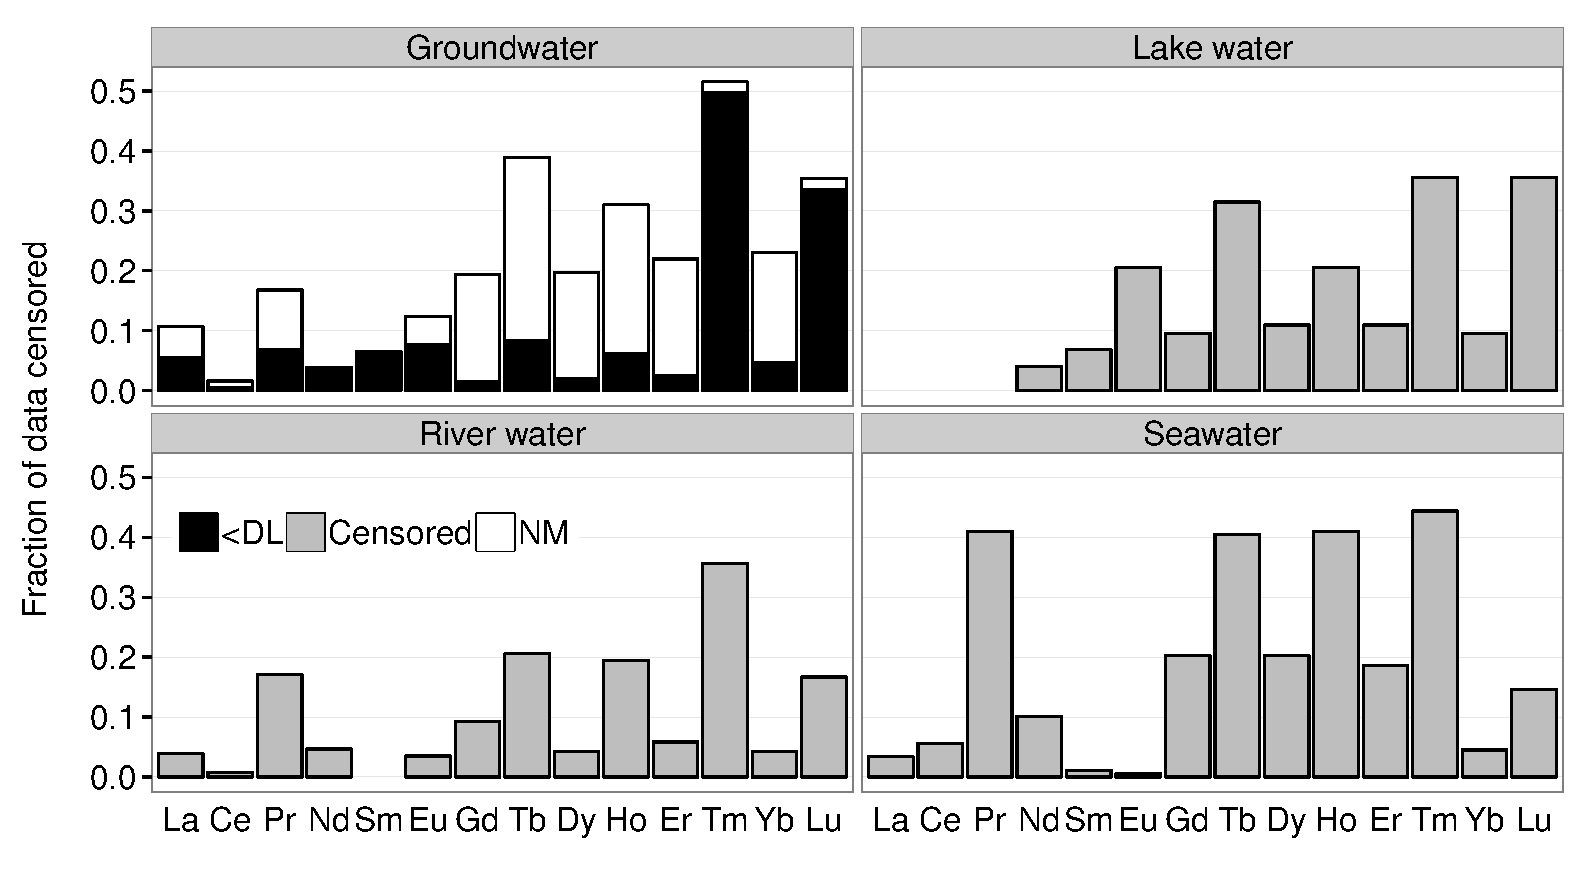
\includegraphics[width=\textwidth]{Ch3_figures/REE-waters-nonDet-type.pdf}
\caption{Fraction of below detection limit ($<$DL) or missing data (NM) for 14 REE in data sets for water types studied. For water types other than groundwater, censored data were not differentiated as below detection or missing, and are lumped together as ``censored''.}\label{fig:cen_frac}
\end{center}
\end{figure}


An additional complexity of this data set was the uneven distribution of data points between data sets (Figure~\ref{fig:sample_dist}).
For example, some data sets included more than seventy samples, while other contained fewer than ten.
This uneven distribution can bias calculated statistics towards studies with a higher number of samples, giving larger studies more weight than smaller studies \citep{Singh_JAWMA_2013}.

\begin{figure}[htbp]
\begin{center}
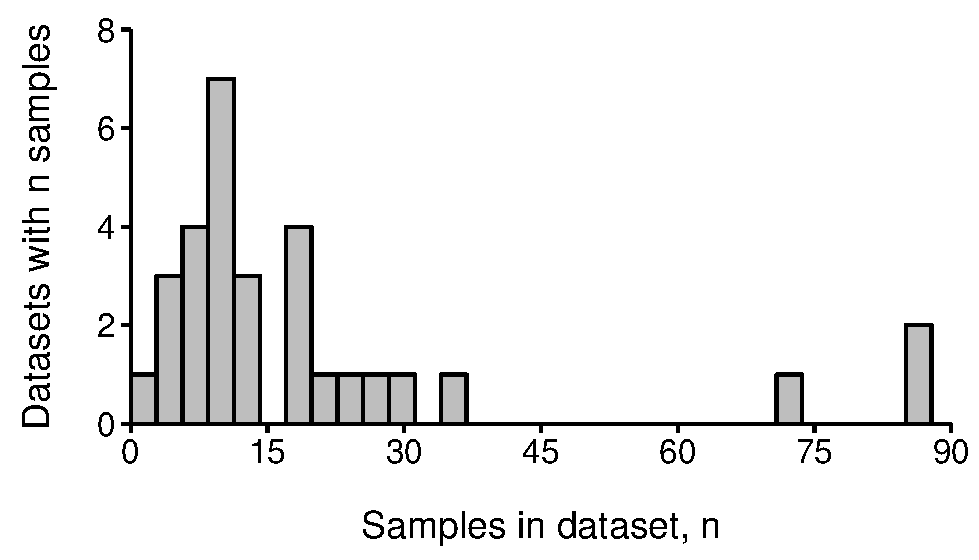
\includegraphics[width=0.8\textwidth]{Ch3_figures/cite-n-dist.pdf}
\caption{Histogram of sample distribution in groundwater dataset (compiled from 31 articles).}\label{fig:sample_dist}
\end{center}
\end{figure}

Censored data were stored at the study-specific MDL with a separate binary variable indicating that the data were censored. Missing data -- that is where REE were either not measured, not reported, or where an MDL was not specified -- were excluded from calculations because nothing was known about the data point in relation to the rest of the data.

Summary statistics were calculated using a weighted Kaplan-Meier (KM) estimator of the survival function accounting for both left-censored and source-size bias.
A routine based on the methodology of Singh, et al. \citep{Singh_JAWMA_2013} was written in \texttt{R} \citep{R} to perform the necessary calculations.
Distribution percentiles were estimated as the first value with a calculated percentile less than the percentile of interest;
stated differently, if the calculated survival quantiles, $S(x)$, for adjacent observations were $S(x_1)=0.94$ and $S(x_2)=0.96$, then $x_1$ would be noted as the 95$^{th}$ percentile.
For data sets with a limited number of samples (e.g. brines) where the sample size or censoring frequency limited the number of calculable percentiles, a log-normal distribution was fit to the KM survival curve by regression on order statistics (ROS) and was used to estimate those percentiles.
Mean values, $\mu_{KM}$, were calculated from the area under the survival curve and standard deviations, $\sigma_{KM}$, from the variance of the mean \citep{Helsel_book}.

The survival curve was approximated using a weighted KM estimator, which considers non-detect data and provides robustness to the uneven distribution of samples from the reviewed literature.
Equation~\ref{eq:wKM} represents the weighted KM estimator, where $\hat{S}(x_i)$ is the probability any observation from the dataset will be \textit{less than} the measured concentration, $x_i$.
In this equation $d_i^w$ represents the weighted count of uncensored observations at concentration $x_i$ and $Y_i^w$ represents the weighted count of all (censored and uncensored) observed concentrations less than $x_i$.
The weight, $w_i$, of each observation is the inverse of the number of samples from the data source ($n_i$), or: $w_i = n_i^{-1}$.
In the absence of weighting or censoring, this formula reduces to the empirical cumulative distribution function.
These calculations, and the relevant \texttt{R} code, are discussed algorithmically in Appendix \textbf{A}.

\begin{align}\label{eq:wKM}
\hat{S}(x_i) = \prod_{x \geq x_i}\left(1 - \frac{d_i^w}{Y_i^w} \right)
\end{align}

Uncertainty in this estimate ($\sigma_{\hat{S}}(x_i)$), expressed using Greenwood's formula \citep{Helsel_book}, is defined by Equation~\ref{eq:greenwood}. As with Equation~\ref{eq:wKM}, $d_i^w$ represents the weighted count of uncensored observations at concentration $x_i$ and $Y_i^w$ represents the weighted count of all observed concentrations less than $x_i$.

\begin{align}\label{eq:greenwood}
\sigma_{\hat{S}}(x_i) = \hat{S}(x_i)\sqrt{\sum_{j=1}^k\frac{d_j^w}{Y_j^w (Y_j^w - d_j^w)}}
\end{align}

Total dissolved REE concentrations were calculated with consideration of censored data.
Rather than calculating the KM survival curve and $\mu_{KM}$ for an individual element (where each sample is an observation) the survival curve was calculated for individual samples (where each REE is an observation).
The sum was determined as follows \citep{Helsel_book}:

\begin{align}\label{eq:totalREE}
\sum [REE] = 14\times \mu_{KM}
\end{align}

 
In addition to univariate summary statistics, inter-element correlations are significantly influenced by the high degree of censoring within the REE data.
Using Pearson's $r$ (linear, least-squares correlation) as an estimate of the correlation would require substitution for censored or missing values \citep{Helsel_EST_1995}, while also making assumptions about the relationship between the variables.
Instead, the Kendall's $\tau$ statistic enabled incorporation of censored data, diminished the influence of outliers (by being robust to log-transformation), and assessed monotonic relationships beyond simple linear relationships.
Thus Kendall's $\tau$ was used for assessing relationships between any variables with multiple censoring levels (detection limits).
The Kendall's $\tau$ method will typically produce lower numeric values (often 0.2 units lower for the same strength of correlation) than other measures, which may make interpretation difficult \citep{Helsel_book};
however, Kendall's $\tau$ is the only technique that allows for inclusion of multiple detection limits non-parametrically without substitution or imputation.
Correlations between variables without censoring were evaluated non-parametrically with Spearman's $\rho$.

\subsection{Reference-normalized element anomalies and ratios}

Several reduced dimension variables (RDVs) are calculated from reference normalized data including ratios of the LREE to MREE and HREE, the Ce anomaly, and the Eu anomaly.
RDVs provide a simplified, univariate presentation of multivariate REE data, quantitatively capturing key features of the REE profile, the plot of reference-normalized concentrations versus atomic number.
The Post Archaean Average Shale (PAAS) of Nance and Taylor \citep{PAAS} was used for normalization.

The Ce anomaly ($Ce_N^*$), the ratio of the normalized Ce concentration to an expected normalized value from interpolation of normalized La and Pr concentrations (calculated in this work with Equation~\ref{eq:CeAnom}), is commonly discussed in the REE literature.

\begin{align}\label{eq:CeAnom}
Ce_N^* = \frac{2\cdot [Ce]_N}{[La]_N + [Pr]_N}
\end{align}

The Eu anomaly ($Eu_N^*$) is calculated similarly using measured Eu concentrations and the concentrations of directly neighboring REE (Sm and Gd).
Both anomalies are commonly log-transformed, a convention that was applied throughout this work.

The ratios of reference normalized REE concentrations were here taken to be an average over multiple elements as opposed to single weight group representatives \citep{Stolpe_GCA_2013}.
The LREE included in ratio analyses were La, Pr, Nd, and Sm; the MREE were Gd, Tb, and Dy; and the HREE were Ho, Er, Tm, Yb, and Lu.
Both Ce and Eu were excluded from calculation of ratios.

These anomalies and interelement ratios cannot be reliably calculated for missing or censored data, thus our analyses of RDVs pertain only to the portion of the dataset where all necessary REE have been reported.
This excludes many datasets utilizing isotope dilution mass spectrometry, which cannot measure mono-isotopic elements, and many studies with higher detection limits or poor analytical precision.

\subsection{Geochemical modelling}

A primary goal was to examine the relationship of REE abundance with various bulk solution chemistries in groundwater.
The REE abundance and concentration data from the literature varied by their sample chemical characterization, water sample origin, sampling location, as well as the nomenclature used to classify geologic environments.
To overcome this heterogeneity we employed a quantitative criterion for the classification of data before any statistical analysis was performed.
For groundwater samples, the total dataset ($N = 619$ samples) was screened under the criterion that the samples were fully characterized for major ions (\ce{Na+}, \ce{K+}, \ce{Ca^2+}, \ce{Mg^2+}, \ce{Cl-}, \ce{SO4^2-}, and \ce{HCO3-}/\ce{CO3^2-}) and pH.
These major solution chemistry data were used to calculate ionic strength and activity of the carbonate ion (\ce{CO3^2-}) using the geochemical equilibrium model PHREEQC with the Pitzer database (pitzer.dat) \citep{PHREEQC, PitzerI}.
Considering the wide range of unique systems represented by this dataset we have not pursued modeling of REE solubility limiting reactions.
While such analyses are useful in well-defined systems, and REE speciation is commonly used to investigate mechanisms of REE abundance \citep{Willis_CG_2011, Johannesson_CG_1996, Johannesson_AG_1995},
significantly more information than was reported for most studies would be needed to conduct the analyses and moreover this type of modeling was deemed beyond the scope of the study.

\section{Results and discussion}

\subsection{Occurrence of REE in aqueous media}

Measured concentrations of REE in natural waters are summarized in Figure~\ref{fig:all_waters}.
Reported concentrations of REE in surface- and groundwater spanned ten orders of magnitude, while individual elements fluctuate with atomic number (i.e., the observed ``zig-zag'' pattern).
This fluctuation of abundance is attributable to the Oddo-Harkins rule, which stipulates that, other than hydrogen, elements with even atomic numbers are more abundant than adjacent elements having odd atomic numbers \citep{Harkins};
this fluctuation gives rise to the common practice of normalizing REE data to a reference standard, for example an average shale or chondritic meteorite, which also exhibits the Oddo-Harkins effect \citep{McLennan_GCA_1994}.
Individual REE are distributed log normally (Figure REF) and are highly correlated with one-another (Figure~\ref{fig:REE_ken}).

\begin{figure}[htbp]
\begin{center}
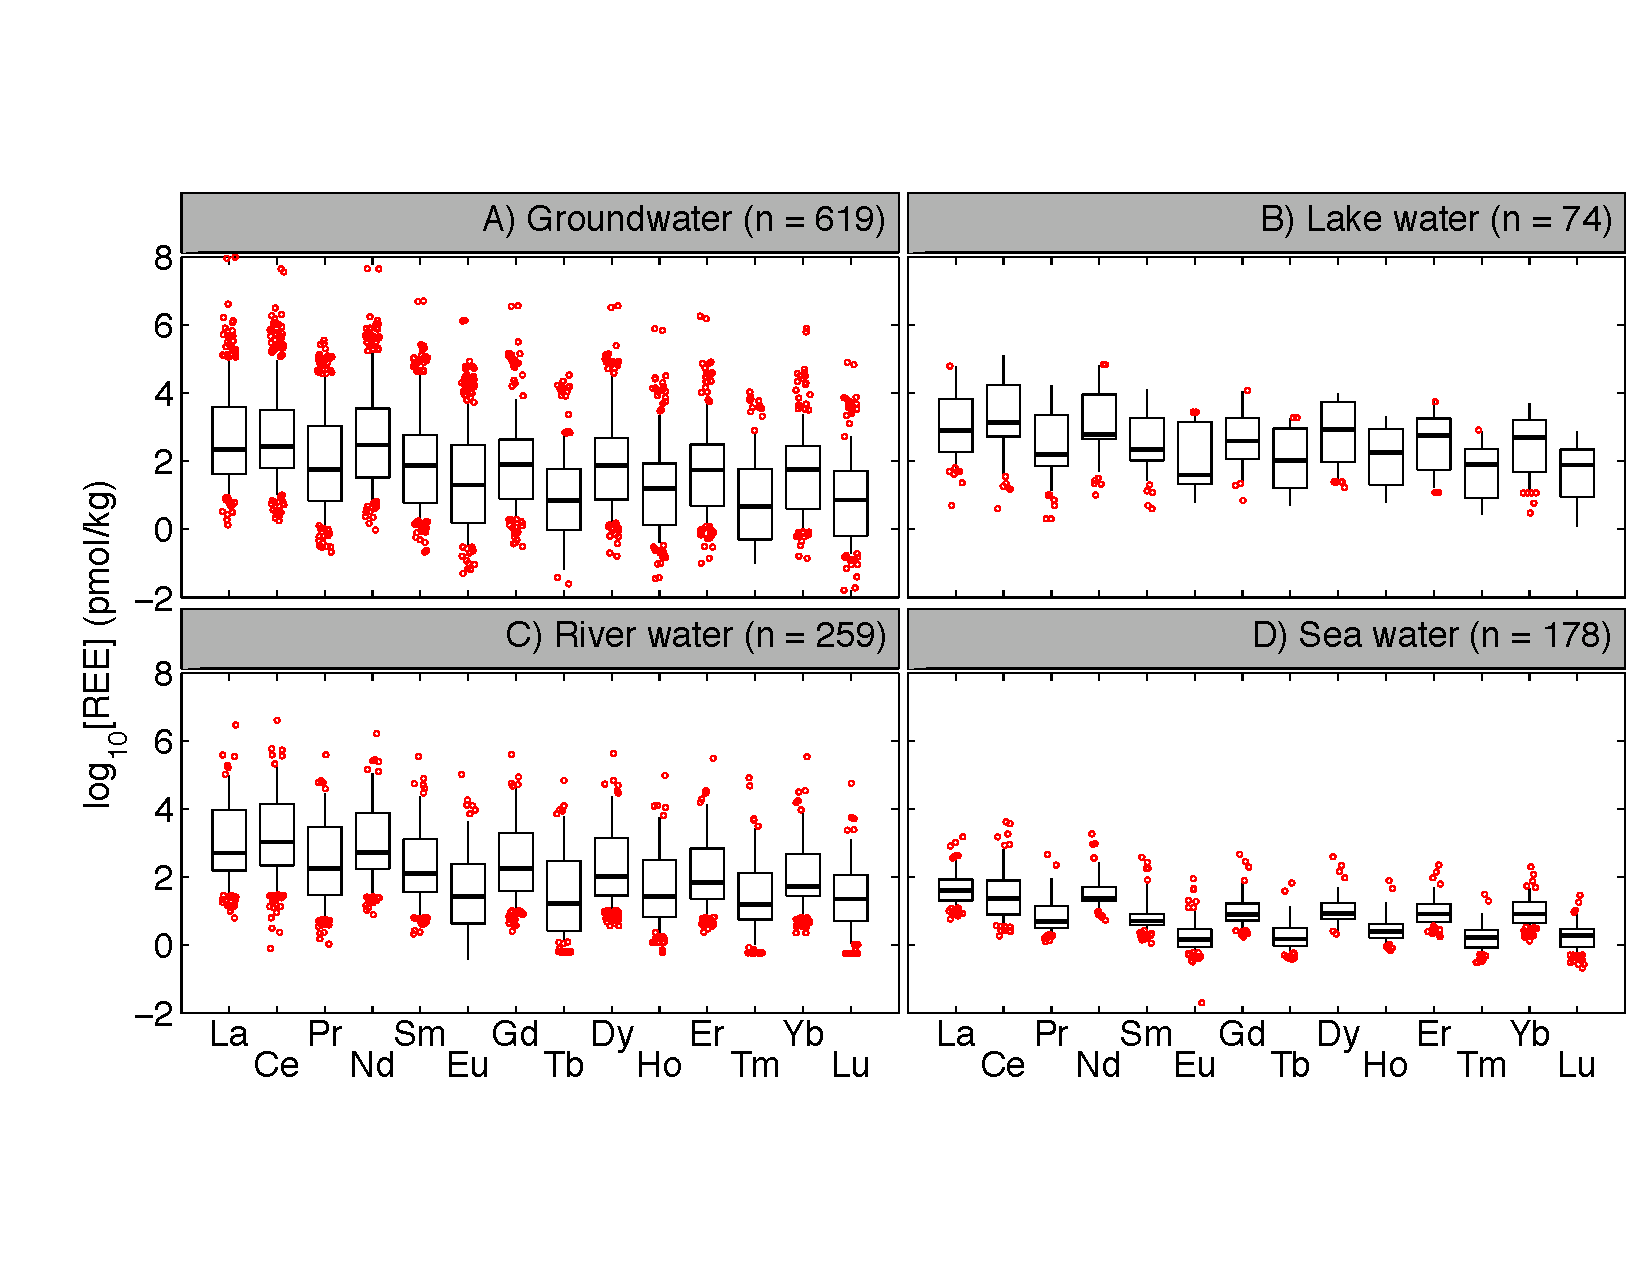
\includegraphics[width=\textwidth]{Ch3_figures/REE-water-boxplot.pdf}
\caption{REE concentration distributions in waters of different types.
Boxplots are based on source-size weighted Kaplan-Meier estimates of REE concentration percentiles and represent the median (thick, black line), inter-quartile range (IQR; first to third quartile; boxed range), 5th to 95th percentile range (whiskers), and remaining outliers (red circles).
In each subfigure heading, ``n'' in the parenthesis denotes the total number of measurements in each water type The number of detected measurements varies between elements.
These data are inclusive, representing unique water sources, spatial and temporal variations within an individual water, and any duplicate analyses.}\label{fig:all_waters}
\end{center}
\end{figure}

\begin{figure}[htbp]
\begin{center}
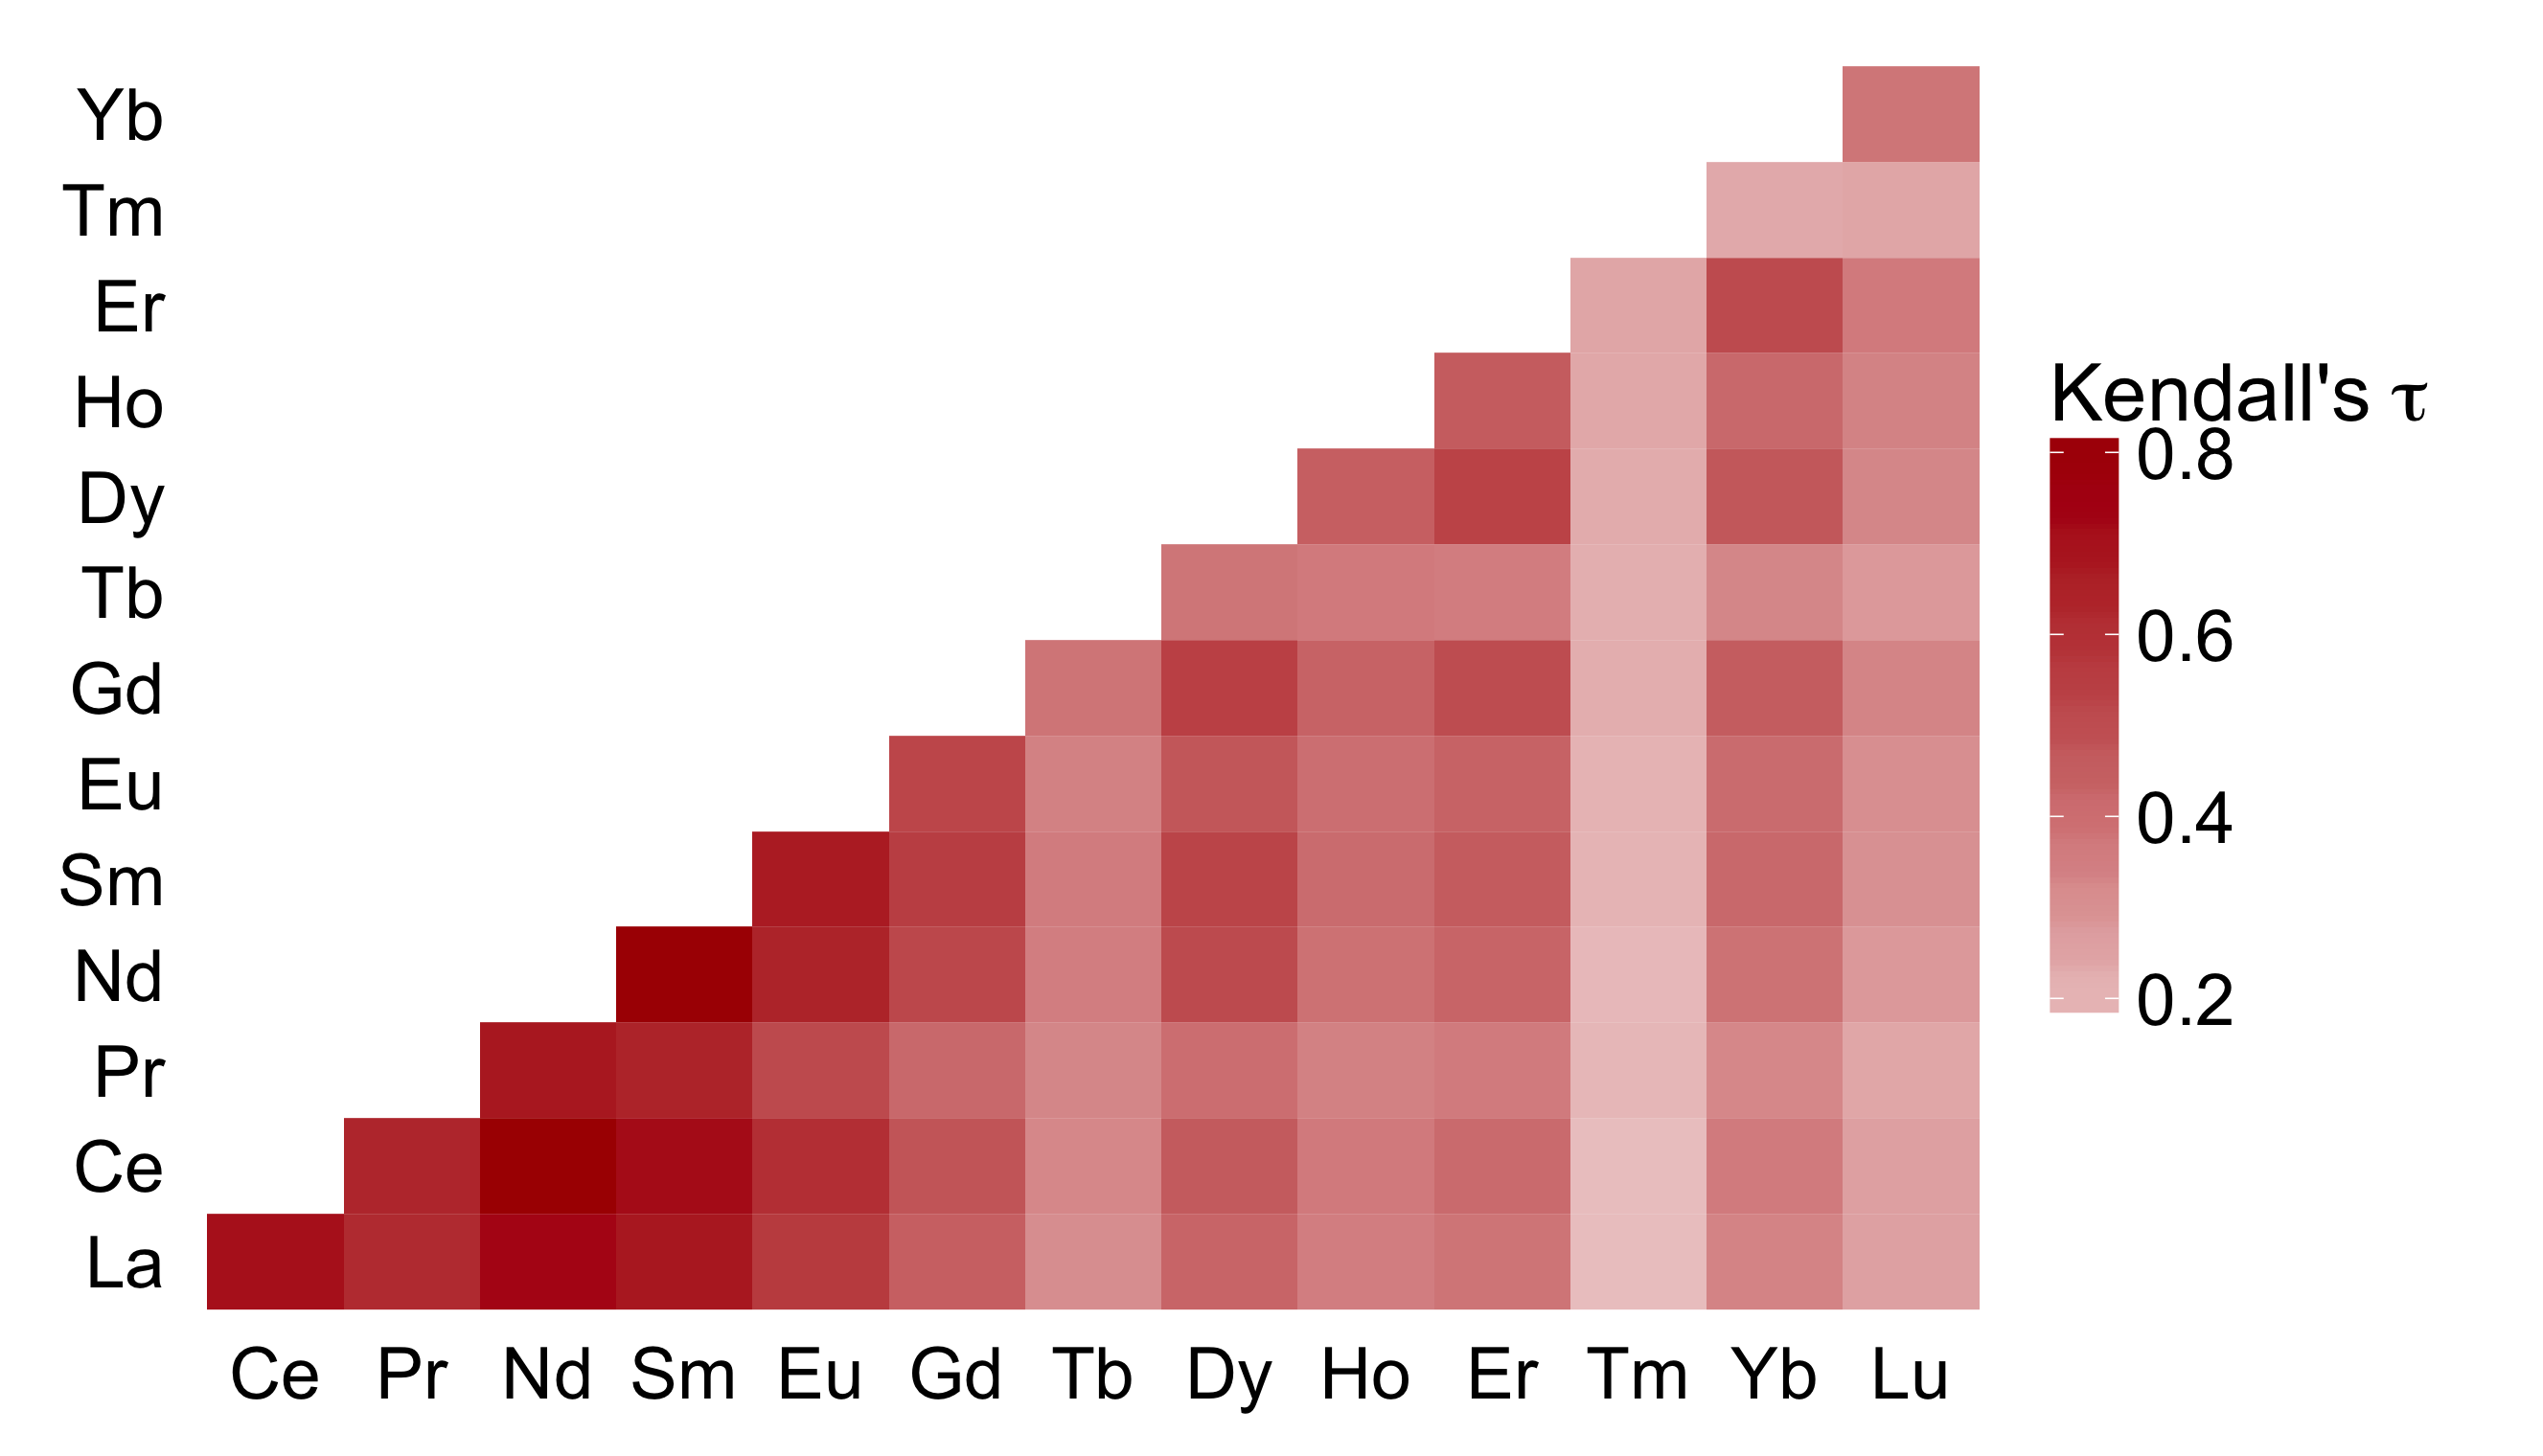
\includegraphics[width=\textwidth]{Ch3_figures/GW-ken-tau.png}
\caption{Heatmap visualization of Kendall's $\tau$ correlation coefficients among the REE in the groundwater dataset.
All correlations are statistically significantly positive.}\label{fig:REE_ken}
\end{center}
\end{figure}

\subsubsection{Groundwater}

In groundwater, the KM-calculated interquartile ranges (KM-IQR, first and third quartile) of overall REE concentrations vary between 5.7 and 410 pmol/kg solution (pmol/kg; Figure~\ref{fig:all_waters}A).
The mean concentration of the groundwater dataset was $3.5 \times 10^4$ pmol/kg and the median was 53 pmol/kg.
As shown in the disparity between the mean and median, REE concentrations in groundwater were heavily right-tailed with many ``outlier'' values and a maximum of $9.7 \times 10^6$ pmol/kg \citep{Miekeley_JGE_1992}.
The REE profile of a groundwater is thought to arise either from water-rock interactions \citep{Willis_CG_2011, Smedley_GCA_1991}
or by changes in the aqueous chemistry \citep{Dia_GCA_2000},
e.g., in relation to the residence time within the aquifer \citep{Johannesson_GW_1997, BwireOjiambo_AG_2003}.

By comparison, substitution of censored data between 0 and 100\% of the detection limit values (without source weighting) results in medians ranging from 4.4 to 13 pmol/kg and mean values ranging from $4.7 \times 10^4$ to $4.9\times 10^4$ pmol/kg.
Alternatively, deletion of below detection data roughly doubles all KM summary statistic estimates: 120 and $5.3\times 10^4$ pmol/kg for median and mean respectively.
Linear interpolation to fill in censored data also leads to significant error (Figure~\ref{fig:interp_error}).
This highlights the criticality of applying appropriate tools in calculating relevant summary statistics, particularly for quantitative analysis.

\begin{figure}[htbp]
\begin{center}
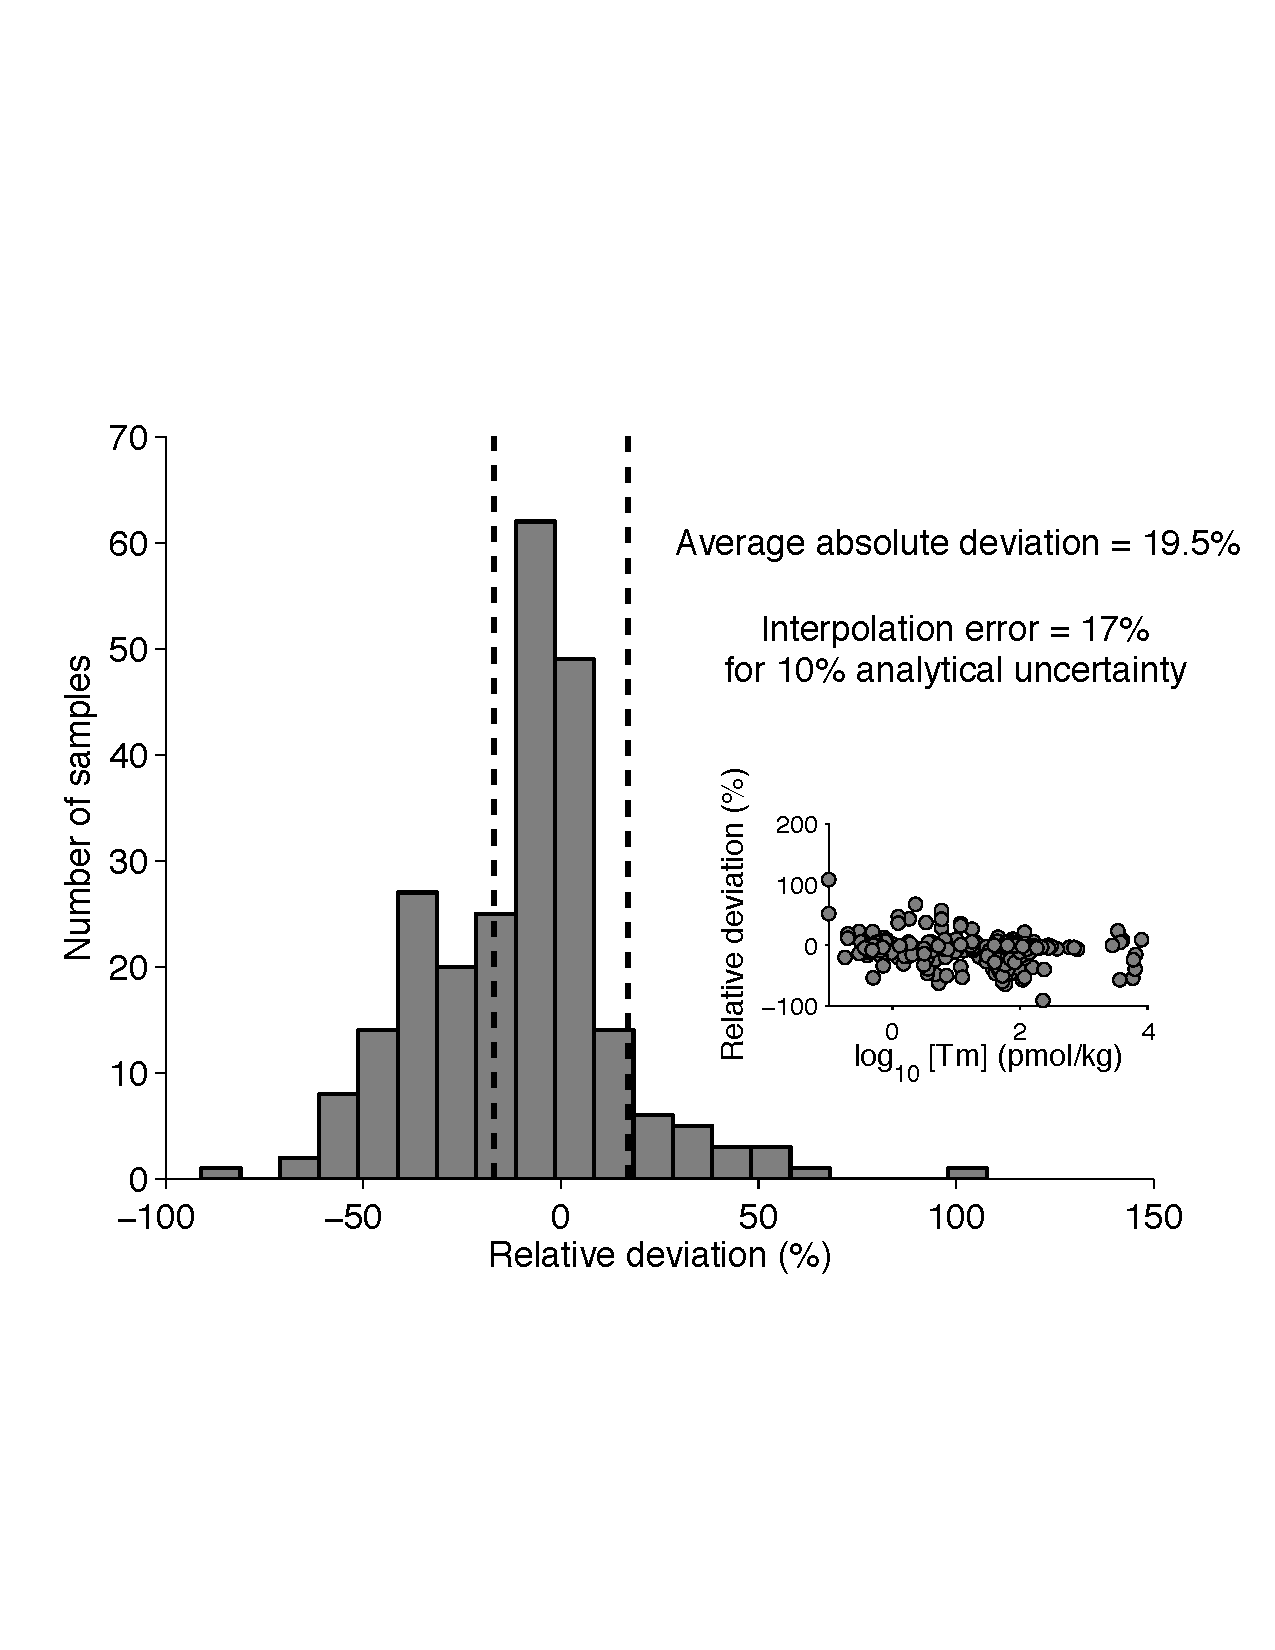
\includegraphics[width=0.8\textwidth]{Ch3_figures/Tm-interpolation-error.pdf}
\caption{Histogram of relative Post Archaean Averaged Shale normalized interpolation error of Tm in groundwater dataset and (inset) dependence of error on measured Tm values.
PAAS normalized Er and Yb were used to ``guess'' the Tm concentration and then compared to the actual measured Tm concentrations. Dashed lines mark the bounds of 10\% analytical uncertainty propagated through the interpolation.
In this analysis 42\% of 241 samples exhibit interpolation error outside the bounds of analytical uncertainty. }\label{fig:interp_error}
\end{center}
\end{figure}

\subsubsection{Terrestrial surface water}

In lake water, the KM-IQR of overall REE concentrations varied between 30 and $1.4\times10^3$ pmol/kg (Figure~\ref{fig:all_waters}B).
The mean concentration of the lake water dataset was $3.8\times10^3$ pmol/kg and the median was 170 pmol/kg.

In river water, the KM-IQRs of overall REE concentrations varied between 15 and 270 pmol/kg (Figure~\ref{fig:all_waters}C).
The mean concentration of the river water dataset was $3.3\times10^3$ pmol/kg and the median was 71 pmol/kg.

\subsubsection{Seawater}

In seawater, the KM-IQR of reported REE concentrations varied between 1.6 and 13 pmol/kg (Figure~\ref{fig:all_waters}D).
The mean concentration of the seawater dataset was 19 pmol/kg and the median was 5 pmol/kg.
The disparity between the dissolved REE in seawater and its influent waters is likely attributable to particulate scavenging \citep{Sholkovitz_GCA_1994, Erel_GCA_1993} at a rate that exceeds mass fluxes from surface- and groundwater sources.
In groundwater by comparison, continuous weathering of the aquifer rock counteracts sorption and co-precipitation loss mechanisms.
Dubinin \citep{Dubinin_LMR_2004} notes that dissolved fractions of REE increase with distance off-shore as terrigenous material settles, which removes REE mass faster than it can be replenished by other sources such as aeolian deposition or hydrothermal venting

\subsubsection{Shale-normalized anomalies and ratios}

The groundwaters in this dataset primarily exhibited mild negative and positive shale-normalized anomalies for Ce and Eu respectively, though, as with abundance, these RDVs varied widely (Figure~\ref{fig:all_RDV}).
Both terrestrial surface waters reported here exhibit similar Ce* and Eu* (Figure~\ref{fig:all_RDV}A and~\ref{fig:all_RDV}B), which are mildly negative and nearly zero respectively.
The Ce* of seawater is starkly different that any of the three water types, developing consistent, negative anomalies with instances of large positive anomalies. 

Nearly all waters in this study are LREE depleted (Figure~\ref{fig:all_RDV}C and~\ref{fig:all_RDV}D).
As with element anomalies, the mean and IQR of interelement ratios among groundwaters and terrestrial surface waters are similar while seawater exhibits distinctly lower ratios.
Both anomalies in groundwater exhibit large outlier values, similar to REE abundance, which underscores the extreme variability in groundwater systems.

\begin{figure}[htbp]
\begin{center}
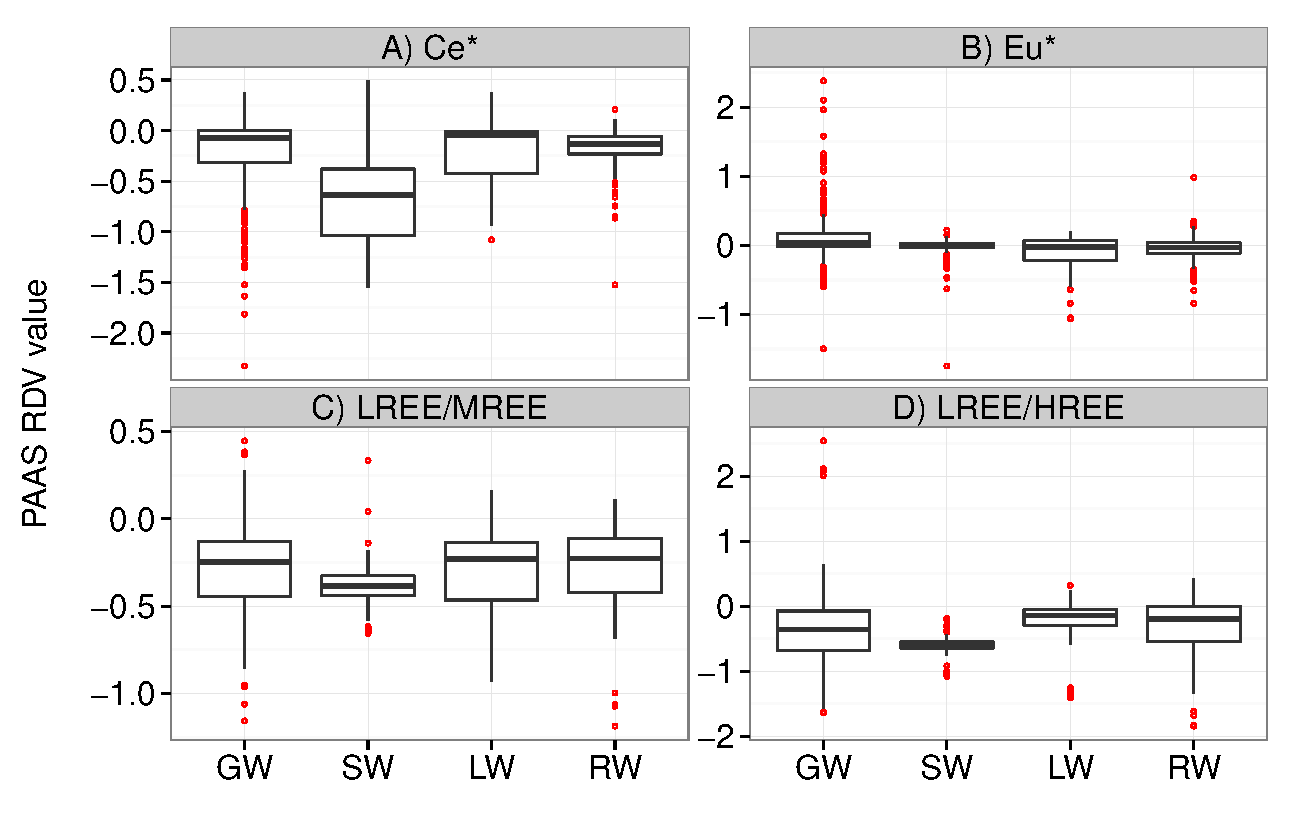
\includegraphics[width=0.8\textwidth]{Ch3_figures/REE-waters-RDV-boxplots.pdf}
\caption{Log-transformed, Post-Archaean Average Shale (PAAS)- normalized, reduced dimension variables (RDVs) calculated for groundwater (GW), seawater (SW), lake water (LW), and river water (RW) data.
RDVs are the cerium anomaly (Ce*), europium anomaly (Eu*), LREE / MREE ratio, and LREE / HREE ratio.
Boxplots represent the median (thick, black line), interquartile range (IQR; first to third quartile; boxed range), $\pm1.5$ times the IQR (whiskers), and remaining outliers (red circles).}\label{fig:all_RDV}
\end{center}
\end{figure}

The anomalies of Ce and Eu are of interest because they are the two REE with redox lability within the Eh-pH regime of water stability \citep{Brookins_GJ_1983}.
Upon oxidation -- Ce(III) to Ce(IV) -- cerium readily precipitates as \ce{CeO2}(s);
alternatively, europium becomes less soluble when reduced from Eu(III) to Eu(II) based on preferential incorporation into other minerals due to the lower valency and higher ionic radius of the reduced state (similar to Sr) \citep{Brookins_RMG_1989}.
Where anomalies in rock samples have been used to infer paleo-redox conditions, the anomalies in aqueous samples are often used to analyze water-rock interactions \citep{Willis_CG_2011, Smedley_GCA_1991}.

Divalent europium is energetically favorable under extremely reducing conditions or at high temperatures.
Reduced Eu(II) exhibits strong partitioning to various minerals during crystallization from magmatic fluids.
Thus many source rocks are either highly enriched (e.g. plagioclase \citep{Nash_GCA_1985}) or highly depleted (e.g. olivine \citep{Foley_Lithos_2004} and pyroxene \citep{Hanson_EPS_1980}) in Eu, enhancing or limiting availability during weathering \citep{Sverjensky_EPSL_1984}.
In hot, reduced, alkaline waters fracture filling calcite commonly contains notable Eu enrichments indicating that the source fluids developed negative Eu* \citep{Lee_AG_2003, Cai_AG_2008}.
However, such environments are representative of hydrothermal waters \citep{Sverjensky_EPSL_1984}, which have specifically excluded from this analysis.
Thus the Eu* in this dataset are thought to result from mineral weathering \citep{Sverjensky_EPSL_1984}.

While aquatic redox couples are commonly in disequilibrium for measured redox potential (Eh) \citep{Linberg_Sci_1984}, Figure~\ref{fig:anom_vs_Eh}A illustrates a negative correlation ($\rho=-0.33$; $P<1\times10^{-6}$) between $Ce_N^*$ and Eh in groundwater, as expected for oxidative scavenging.
However, the low strength of the correlation reflects the mechanism being a function of both source composition and aqueous chemistry.
Europium anomalies do not exhibit the expected positive trend with redox potential in groundwater, though a weak negative correlation is observed ($\rho= -0.18$, $P = 0.006$; Figure~\ref{fig:anom_vs_Eh}B).
Stability diagrams with measure Ce* and Eu* are included in Figure~\ref{fig:pourbaix} and show the lack of agreement between measured and thermodynamically predicted anomalies.

\begin{figure}[htbp]
\begin{center}
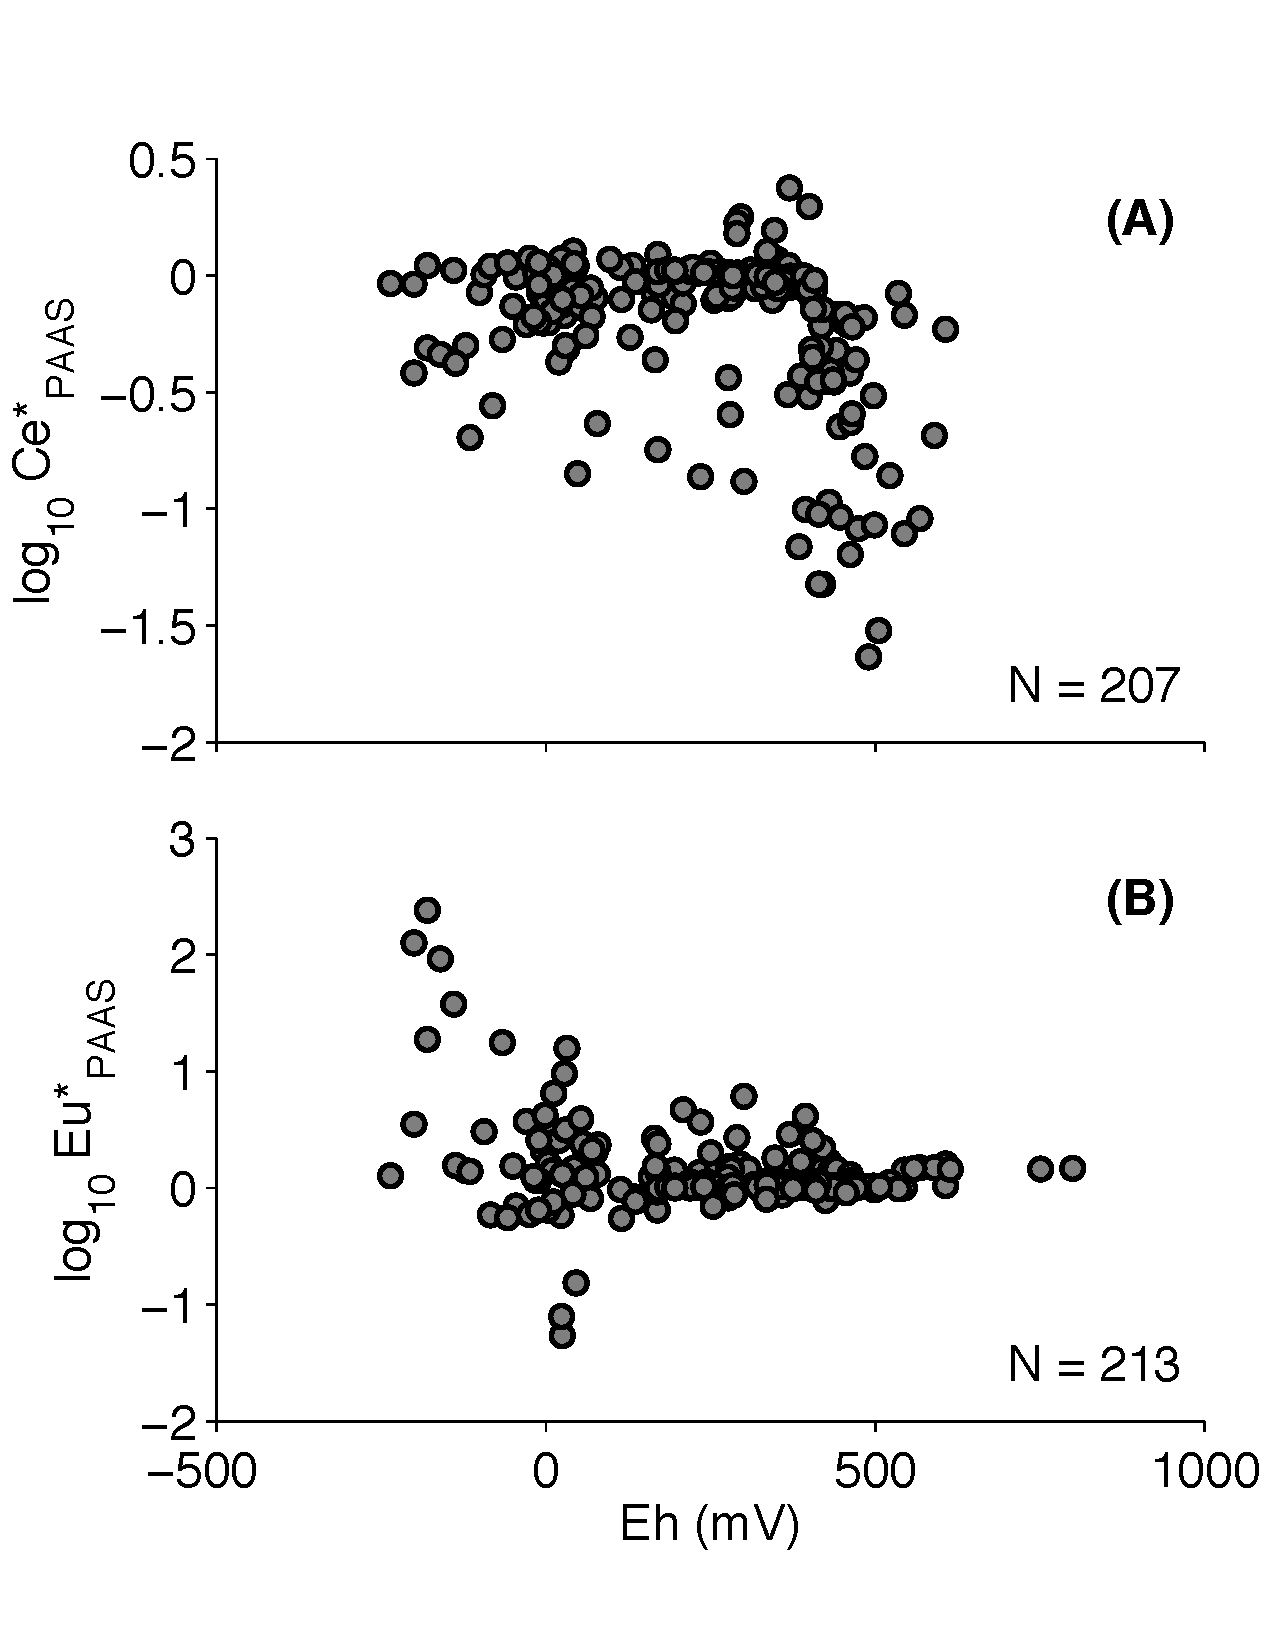
\includegraphics[width=0.5\textwidth]{Ch3_figures/Ce-Eu-anom-vs-Eh.pdf}
\caption{Groundwater Post-Archaean Average Shale (PAAS) Ce anomaly (Ce*, A, Eq.~\ref{eq:CeAnom}) and Eu anomaly (Eu*, B) as a function of reported redox potential (Eh).
Sample size denoted by ``N''.}\label{fig:anom_vs_Eh}
\end{center}
\end{figure}

\begin{figure}[htbp]
\begin{center}
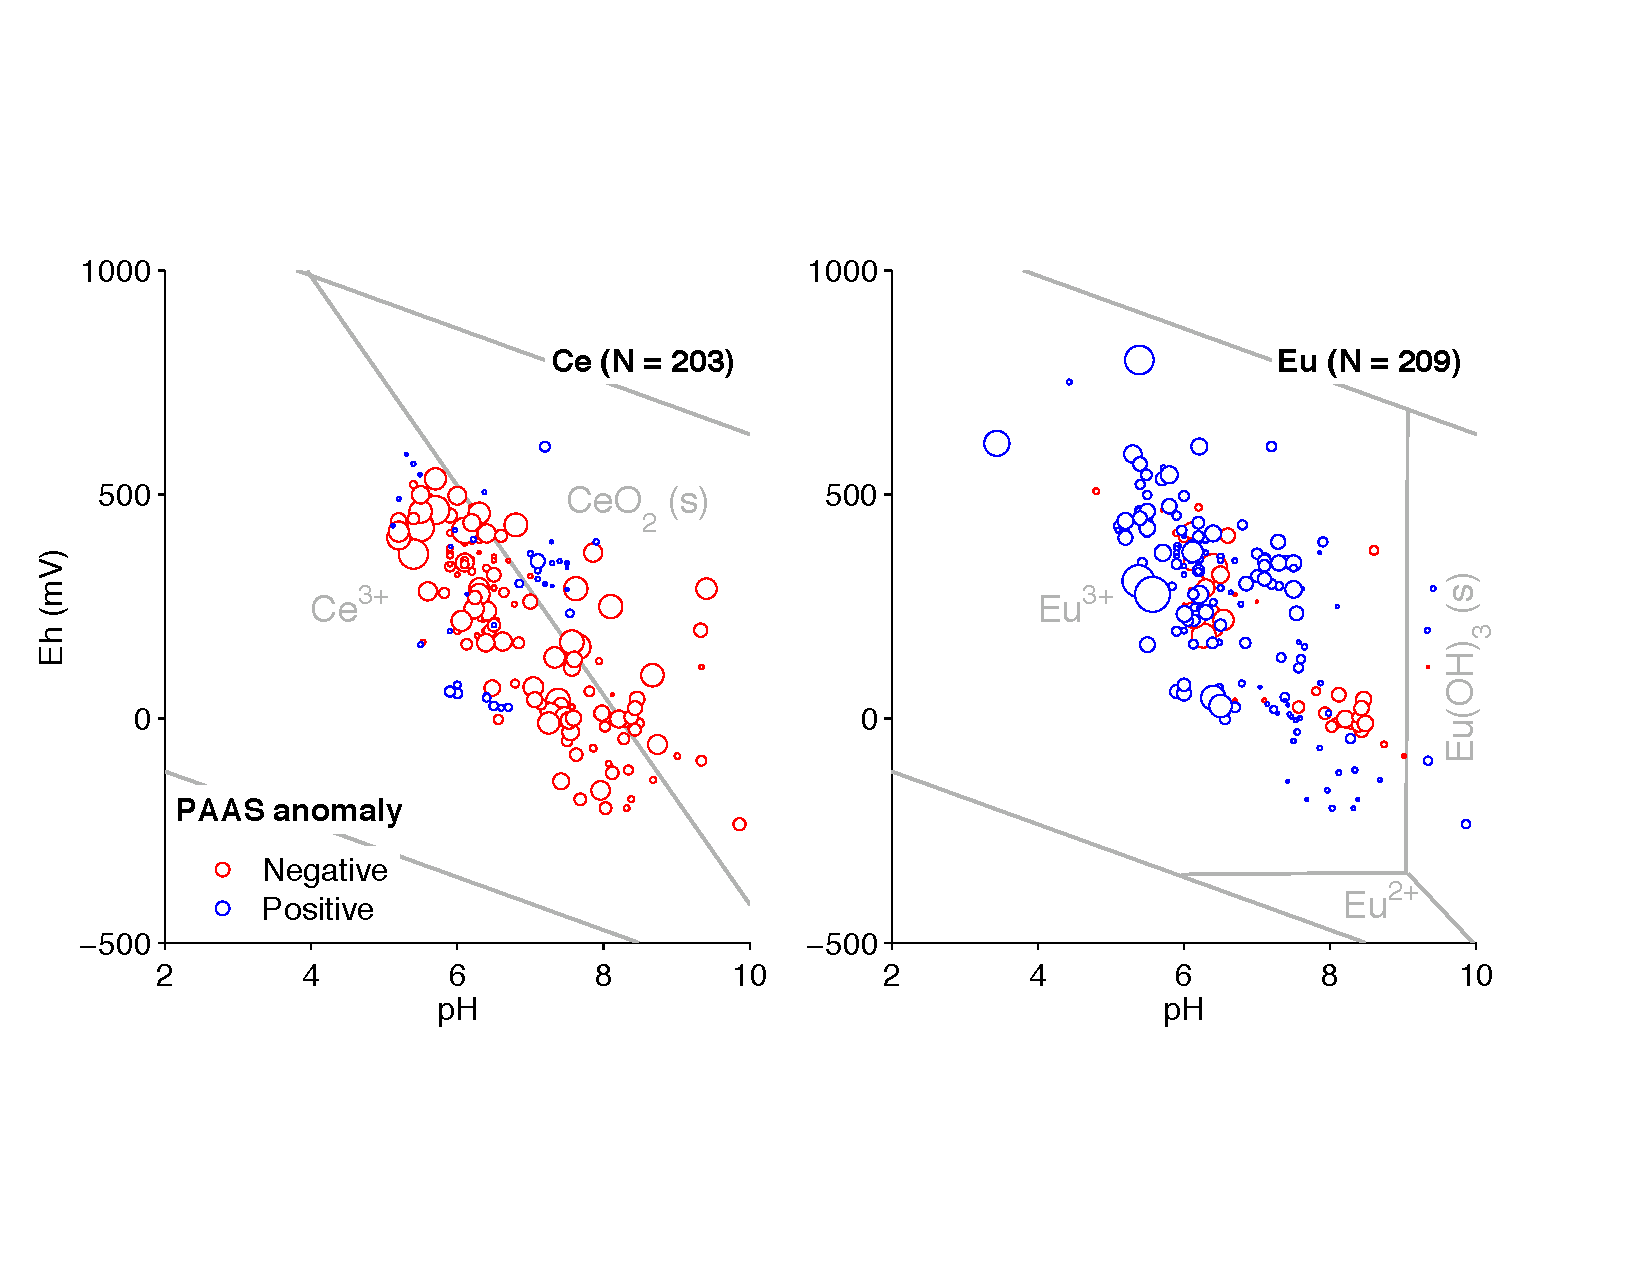
\includegraphics[width=\textwidth]{Ch3_figures/Ce-Eu-stability-anom.pdf}
\caption{Post-Archaean Average Shale (PAAS) Cerium (Ce; left) and Europium (Eu; right) anomalies as functions of redox potential (Eh) and pH.
Marker color corresponds to the sign of the anomaly and marker size corresponds to the magnitude of the anomaly.
Stability fields, reproduced from Brookins \citep{Brookins_RMG_1989}, for relevant species in the REE-\ce{H2O} system underlie the data for TOTCe$=$TOTEu $=10^{-11}$ M at 298 K}\label{fig:pourbaix}
\end{center}
\end{figure}

\subsection{REE abundance trends in groundwater}

Of all the bulk solution chemistry parameters for groundwater, pH exerted the greatest control as an independent variable over dissolved REE abundance (Figure~\ref{fig:sum_vs_pH}). Generally, more acidic waters contained the most REE, either via acidification-enhanced weathering or from an enrichment of REE in the acid source \citep{Dia_GCA_2000, Smedley_GCA_1991, Gosselin_GCA_1992, Janssen_WR_2003, Worrall_AG_2001, Leybourne_AG_2000, Miekeley_JGE_1992}.
REE are effectively scavenged from more neutral and basic waters via sorption onto oxides and clays or co-precipitation with carbonates and phosphates by replacing calcium, which has a comparable atomic radius \citep{Johannesson_LO_1994, CRC_handbook, Bradbury_GCA_2002, Coppin_CG_2002, Quinn_MC_2006, Terakado_CG_1988}.
Over the pH range 4-8, dissolved REE abundance follows an approximate $-1$ slope with increasing pH (95\% confidence interval of $-1.02 \pm 0.1$), indicative of a single-proton (i.e. mono-dentate) surface complexation reaction or calcite precipitation when carbonate far exceeds calcium \citep{Morel_Herring}.
Geochemical modeling showed that nearly all samples were significantly undersaturated with respect to either pure-phase REE hydroxides or carbonates (Figure~\ref{fig:REE_SI}).

\begin{figure}[htbp]
\begin{center}
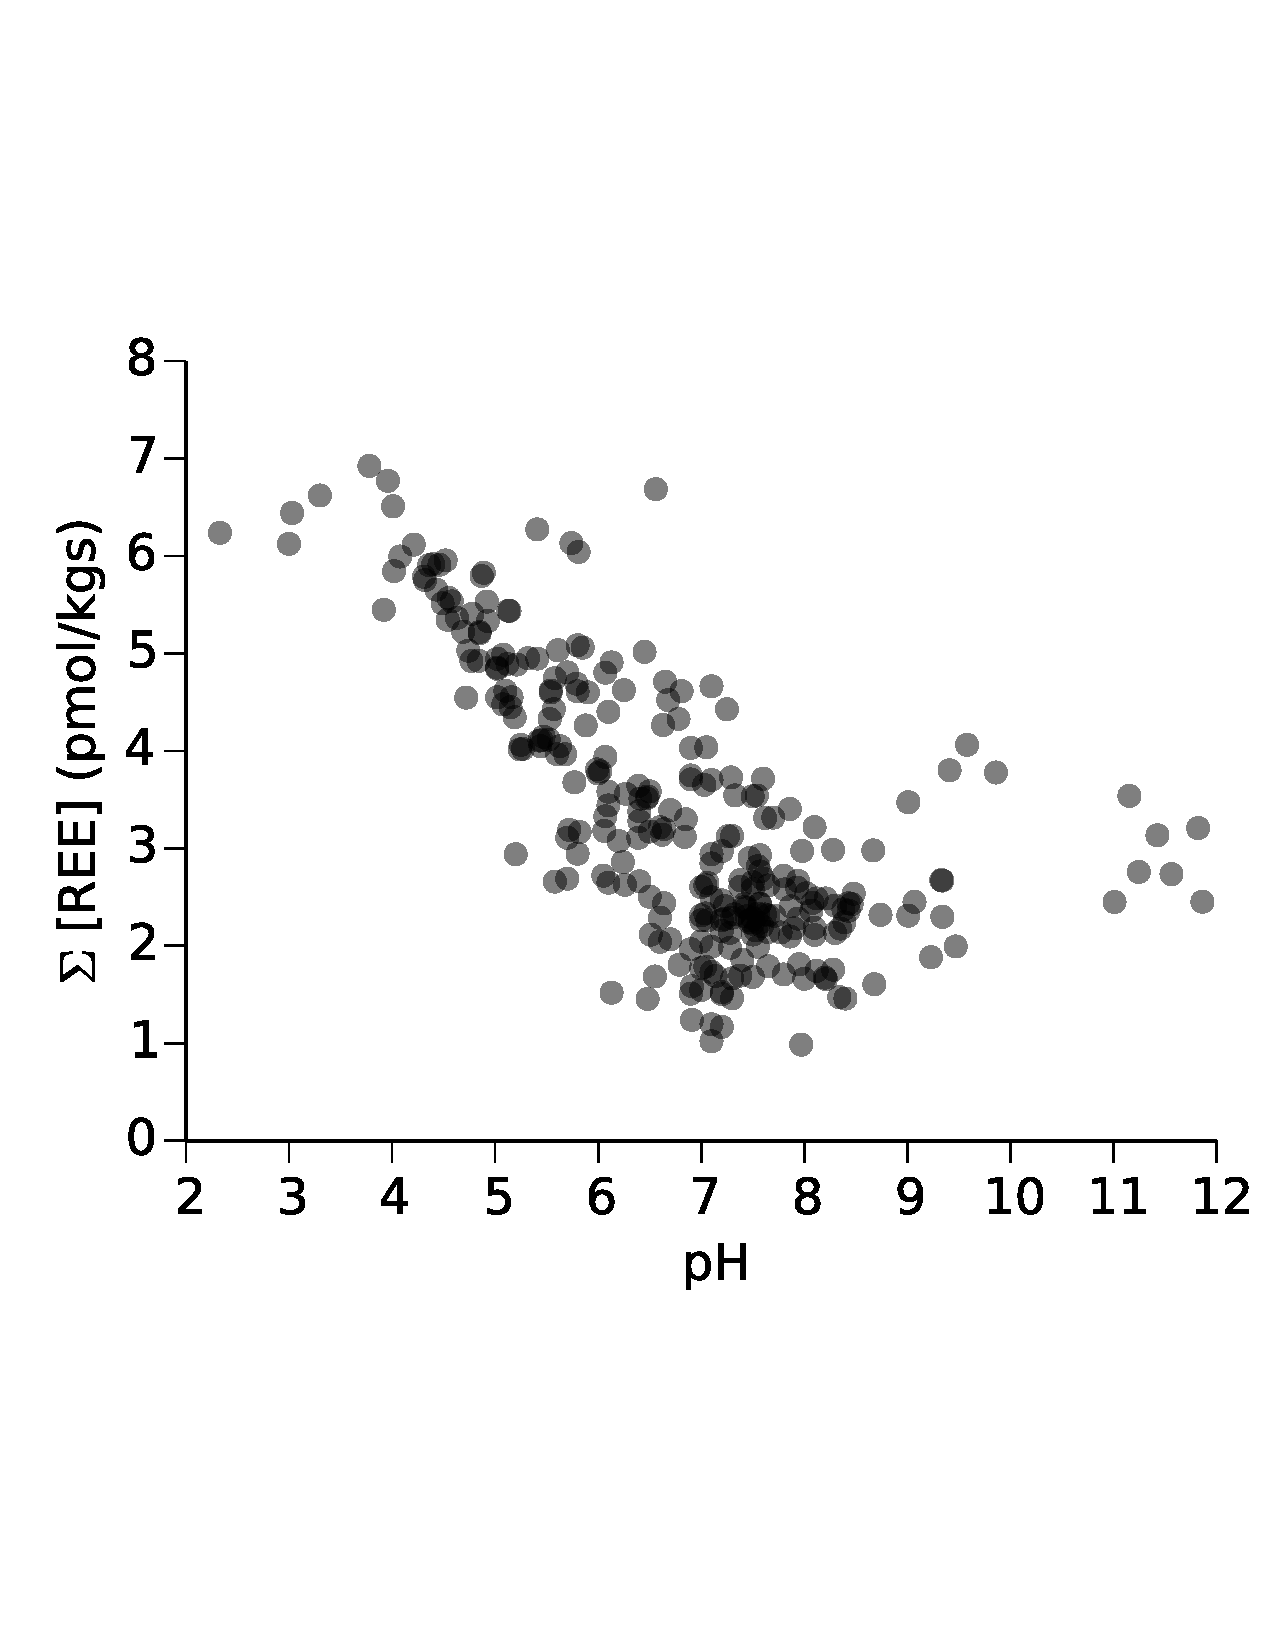
\includegraphics[width=0.67\textwidth]{Ch3_figures/tot_REE-vs-pH.pdf}
\caption{Sum of dissolved REE vs pH for groundwater data from Kaplan-Meier estimates (Eq~\ref{eq:totalREE}).
Markers are semitransparent to illustrate data density.
Data presented for 281 samples.}\label{fig:sum_vs_pH}
\end{center}
\end{figure}

\begin{figure}[htbp]
\begin{center}
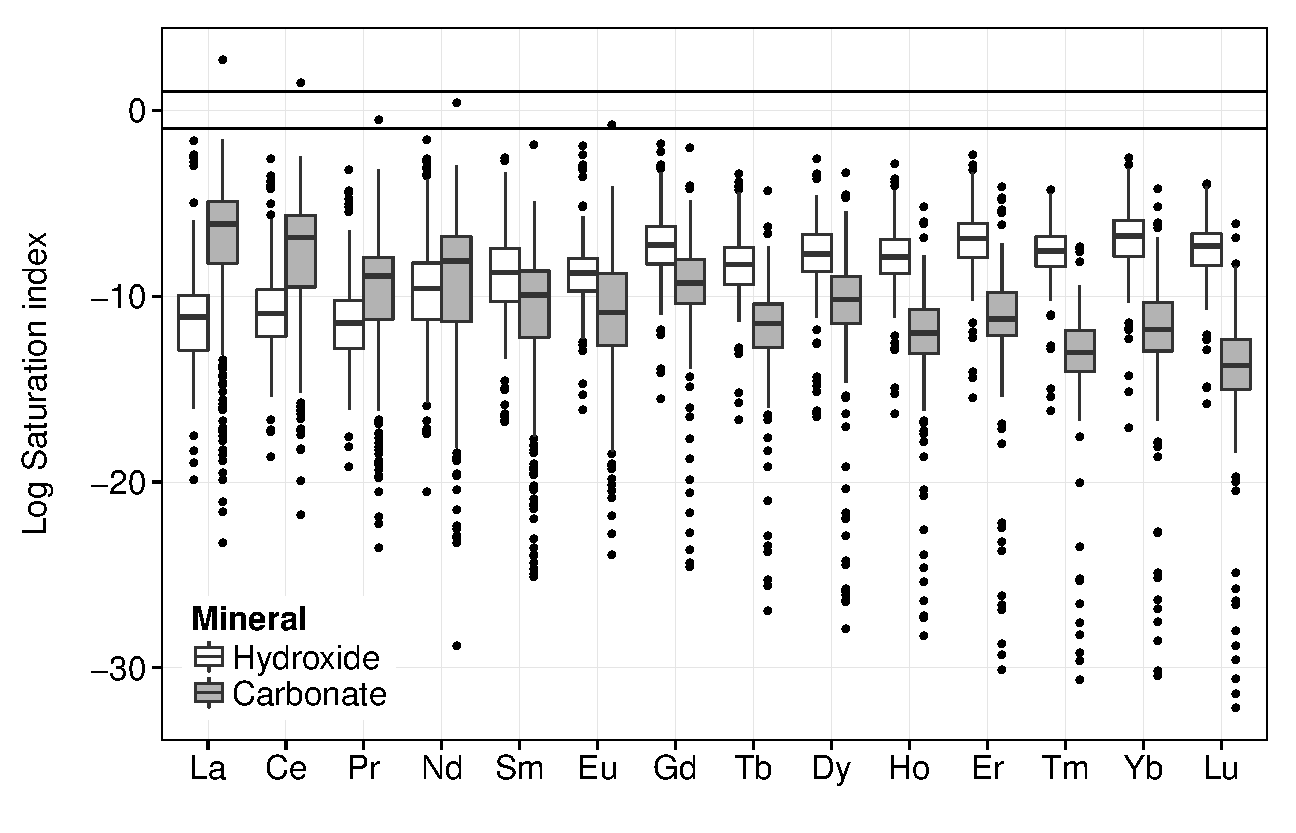
\includegraphics[width=0.8\textwidth]{Ch3_figures/REE-mineral-SI.pdf}
\caption{Modeled, log-transformed saturation indices of pure phase REE hydroxides and carbonates for groundwater data. Saturation indices calculated using PHREEQC and the LLNL database. Solid lines at $-1$ and 1 indicate range of potentially solubility controlling phases \citep{Meima_EST_1997}.}\label{fig:REE_SI}
\end{center}
\end{figure}

Strong complexation with carbonate, particularly as a dicarbonato complex (\ce{REE(CO3)2-}) is thought to account for the apparent amphoteric behavior as pH becomes more  \citep{Millero_GCA_1992, Wood_CG_1990, Johannesson_AG_1995}.
The REE form progressively stronger carbonate and dicarbonato complexes with increasing atomic number \citep{Millero_GCA_1992, Wood_CG_1990}, which would suggest an increase of MREE or HREE relative to LREE as a function of pH or carbonate ion activity.
However, such a trend is not observed within the current dataset (Figure~\ref{fig:frac_vs_acarb}) though the breadth of the current dataset may simply obscure such trends seen in individual studies \citep[e.g. Ref.][]{Choi_CG_2009}.

\begin{figure}[htbp]
\begin{center}
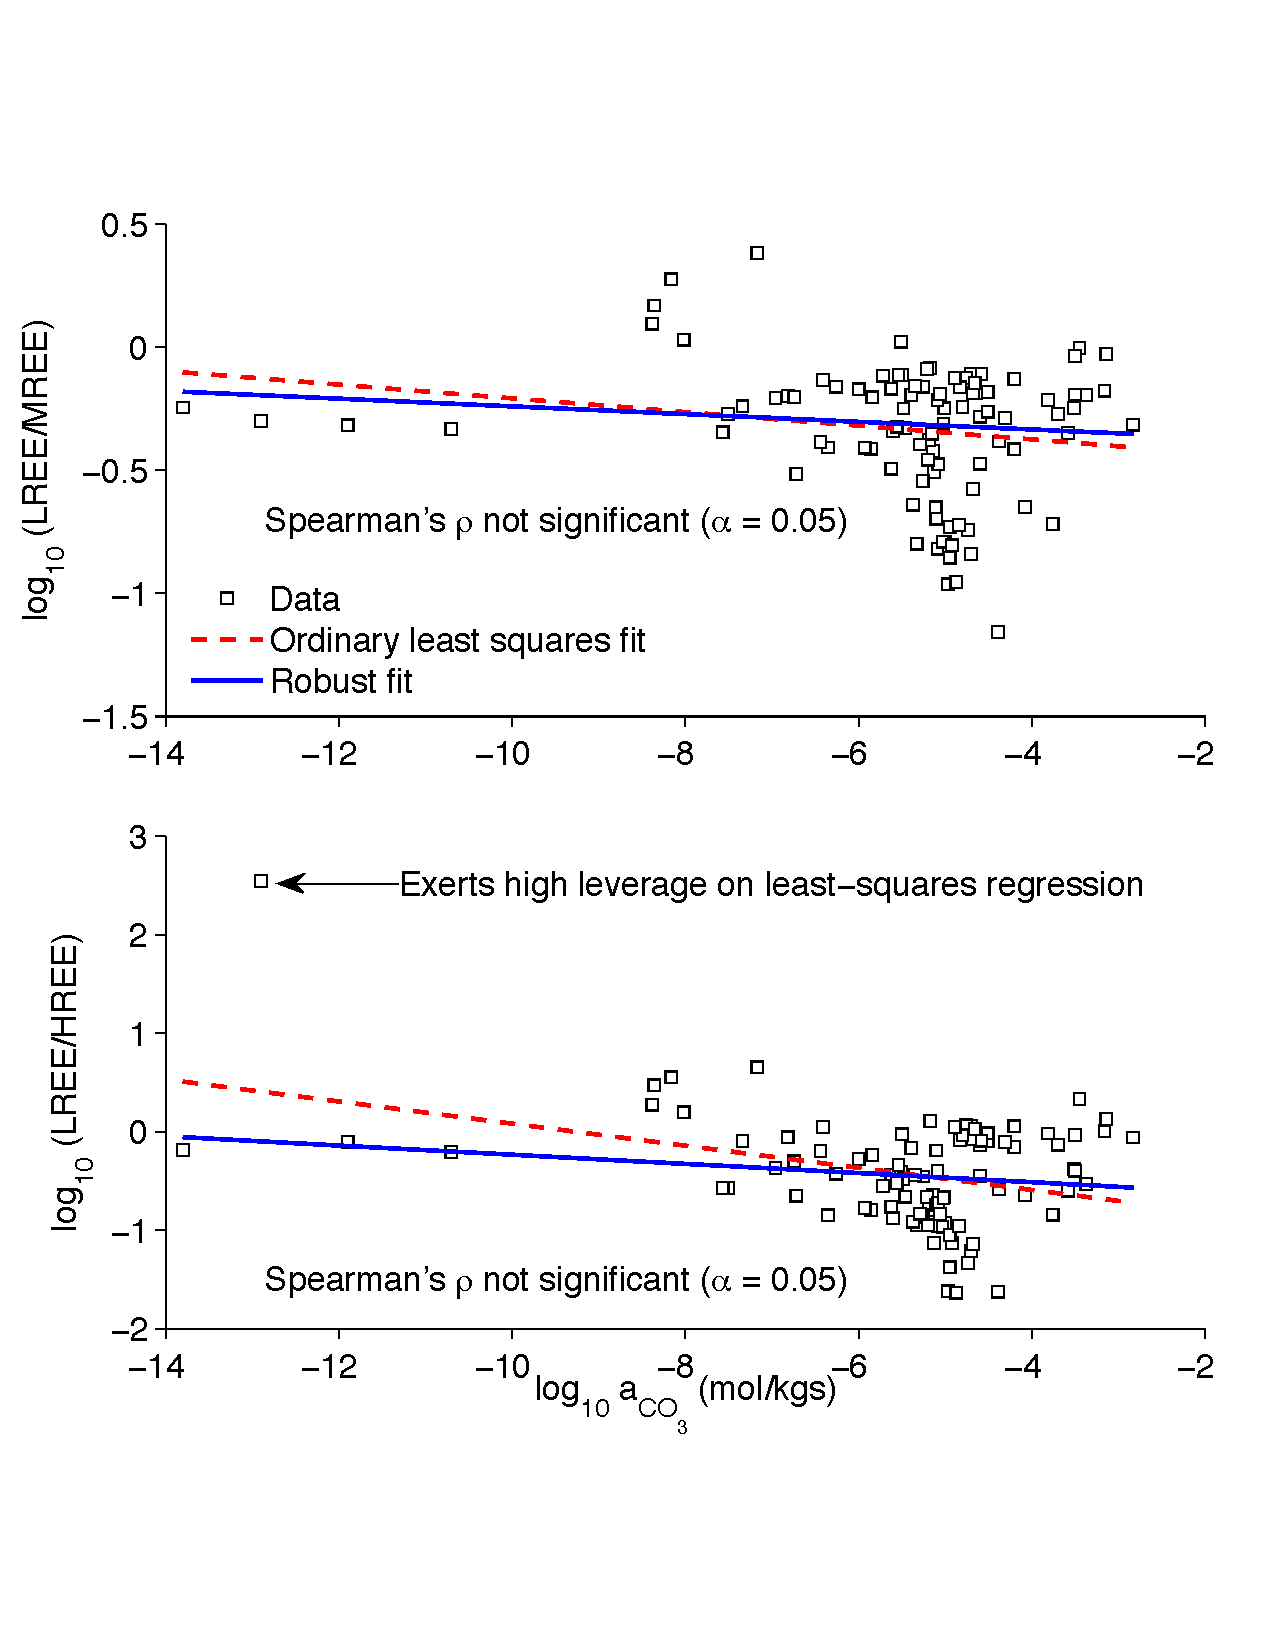
\includegraphics[width=0.8\textwidth]{Ch3_figures/REE-ratios-vs-act_carb.pdf}
\caption{Light-middle REE fractionation (top) and light-heavy REE fractionation (bottom) as a function of modeled carbonate ion activity (a$_{\ce{CO3}}$).
For L/M fractionation neither regression is significant, while L/H ordinary least squares regression is significant due to a high outlier value. Each plot contains 99 data points.}\label{fig:frac_vs_acarb}
\end{center}
\end{figure}

Kendall's $\tau$ correlation analysis of REE with bulk solutes shows inconsistent trends, however most of the meaningful relationships are between the solutes and the LREE and are weakly negative (Figure~\ref{fig:REE-vs-major}).
This behavior is contrary to many other metals that correlate positively with dissolved solids.
This likely highlights the heterogeneity of the dataset and the importance of surface reactions in controlling dissolved REE abundance.

\begin{figure}[htbp]
\begin{center}
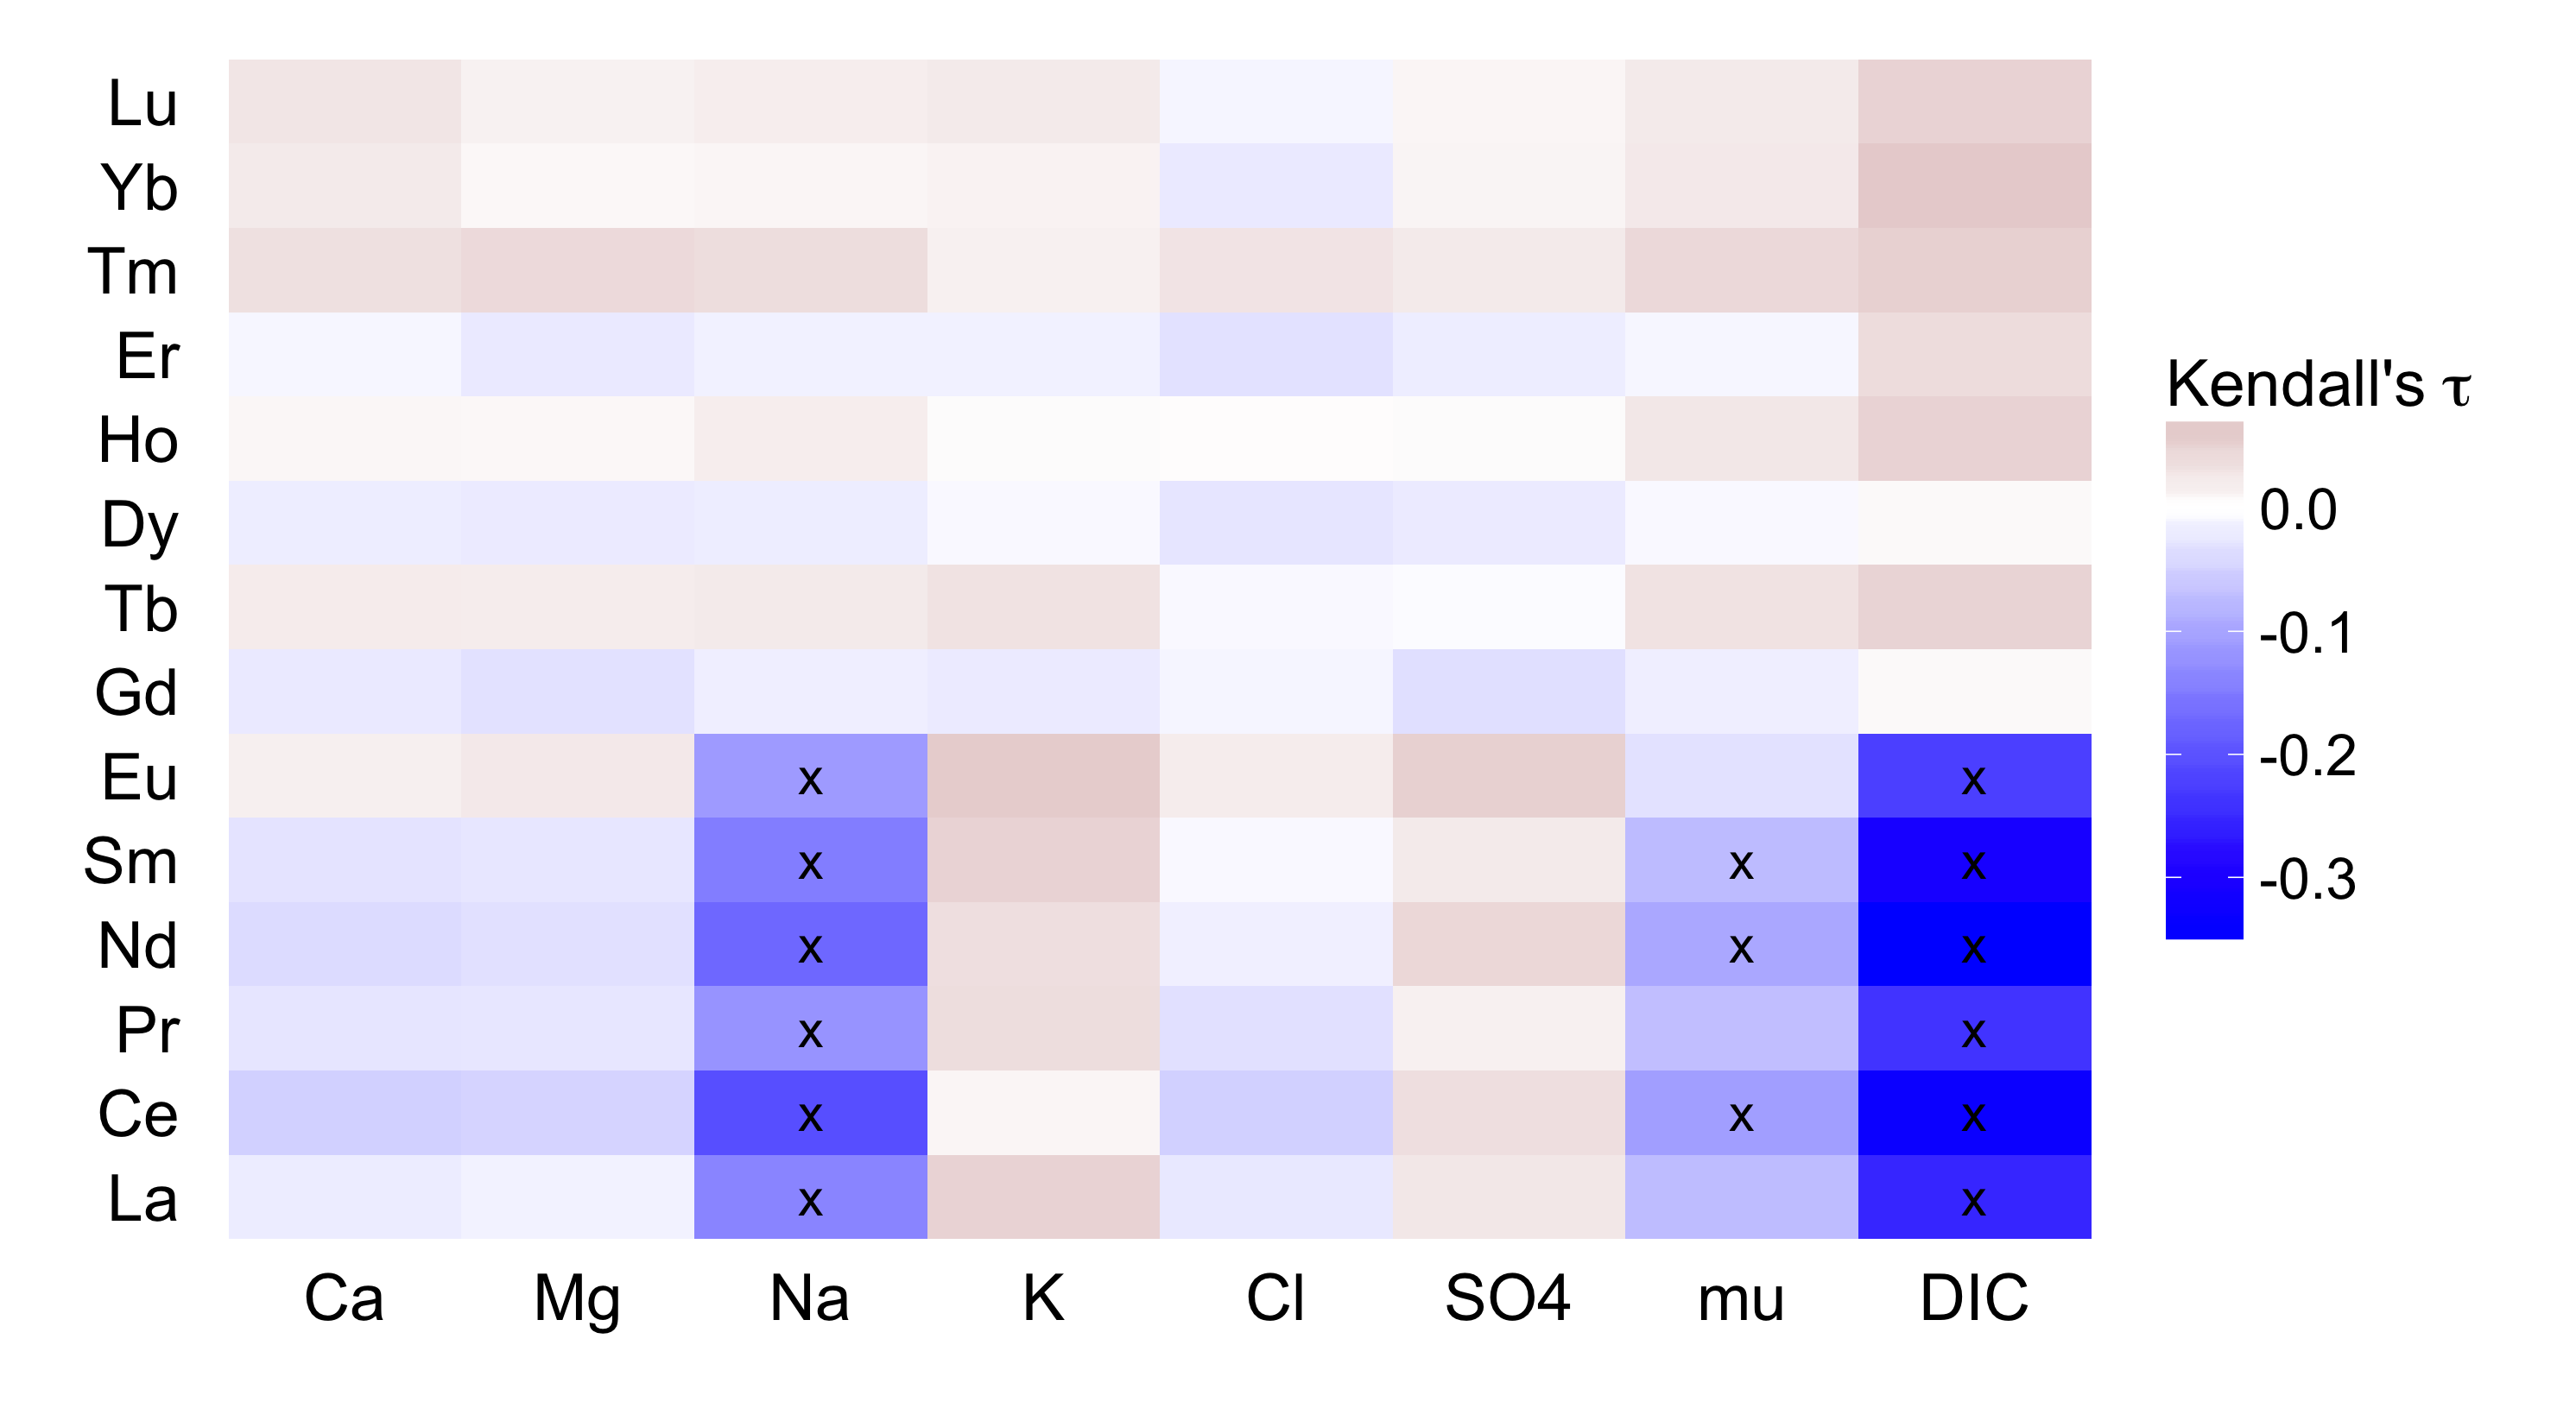
\includegraphics[width=0.9\textwidth]{Ch3_figures/REE-vs-chem.png}
\caption{Heatmap visualization  of Kendall's $\tau$ coefficients between REE abundance and total bulk solutes and calculated ionic strength (``mu'') in groundwater.
Statistically significant correlations ($\alpha = 0.05$) are noted with an ``x''.}\label{fig:REE-vs-major}
\end{center}
\end{figure}

\subsubsection{Major element chemistry of the groundwater data}

For the groundwater data, the screening process reduced the total number of samples from 619 to 328.
The representative chemistries of the screened dataset samples varied widely, with several orders of magnitude range in the major ion concentrations (Figure~\ref{fig:GW-chem-hist}).
Plotting the major ion concentrations using a Piper diagram \citep{Piper_diag} showed that the major anions were predominantly Cl/\ce{SO4}, while the predominant cations varied between monovalent and divalent (Figure~\ref{fig:GW-chem-piper}).

\begin{figure}[htbp]
\begin{center}
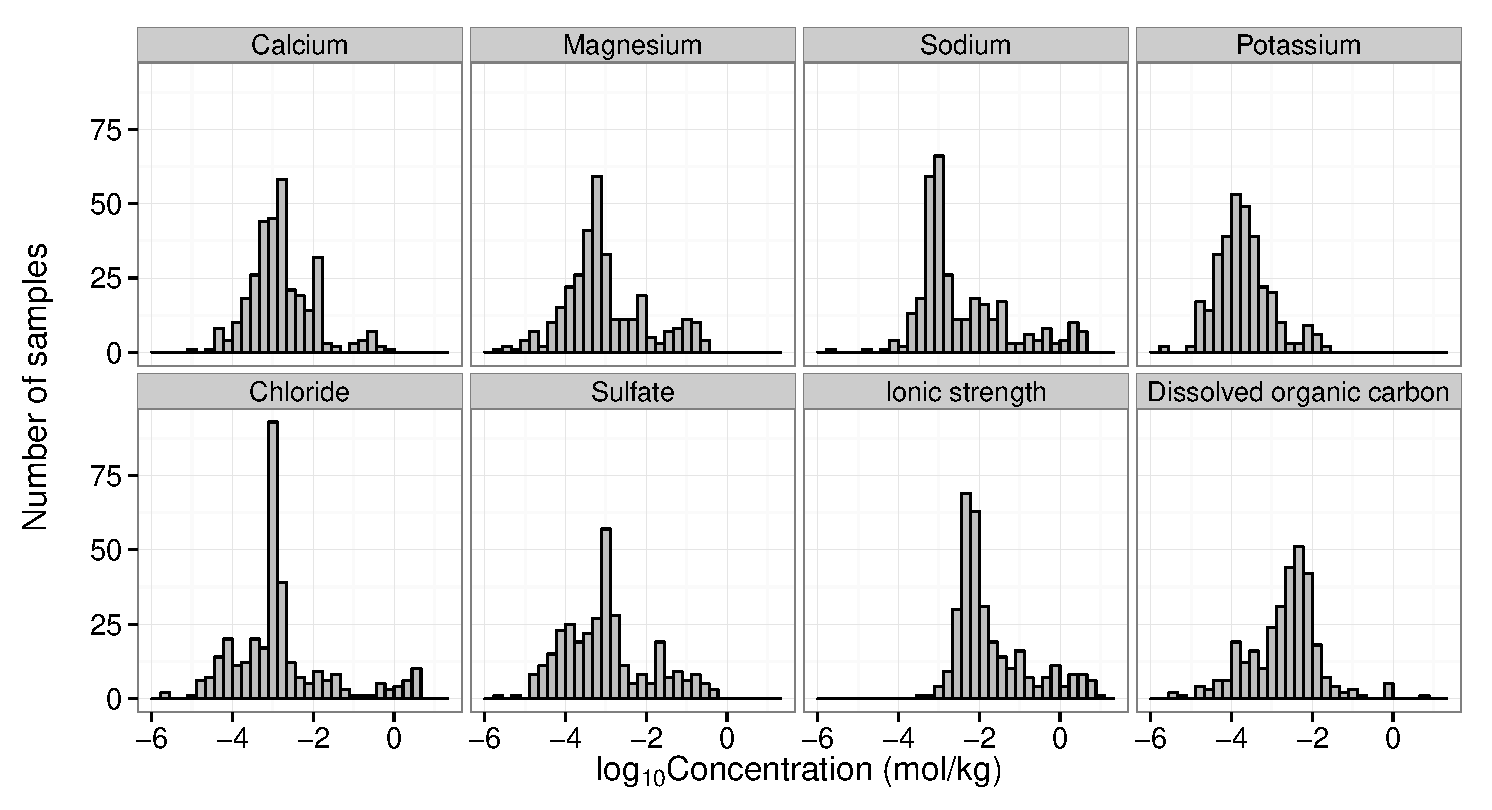
\includegraphics[width=\textwidth]{Ch3_figures/GW-chem-hist.pdf}
\caption{Major solution chemistry histograms for groundwater dataset. Total dissolved inorganic carbon was either given or estimated from alkalinity data using PHREEQC. Ionic strength was calculated using PHREEQC.}\label{fig:GW-chem-hist}
\end{center}
\end{figure}

\begin{figure}[htbp]
\begin{center}
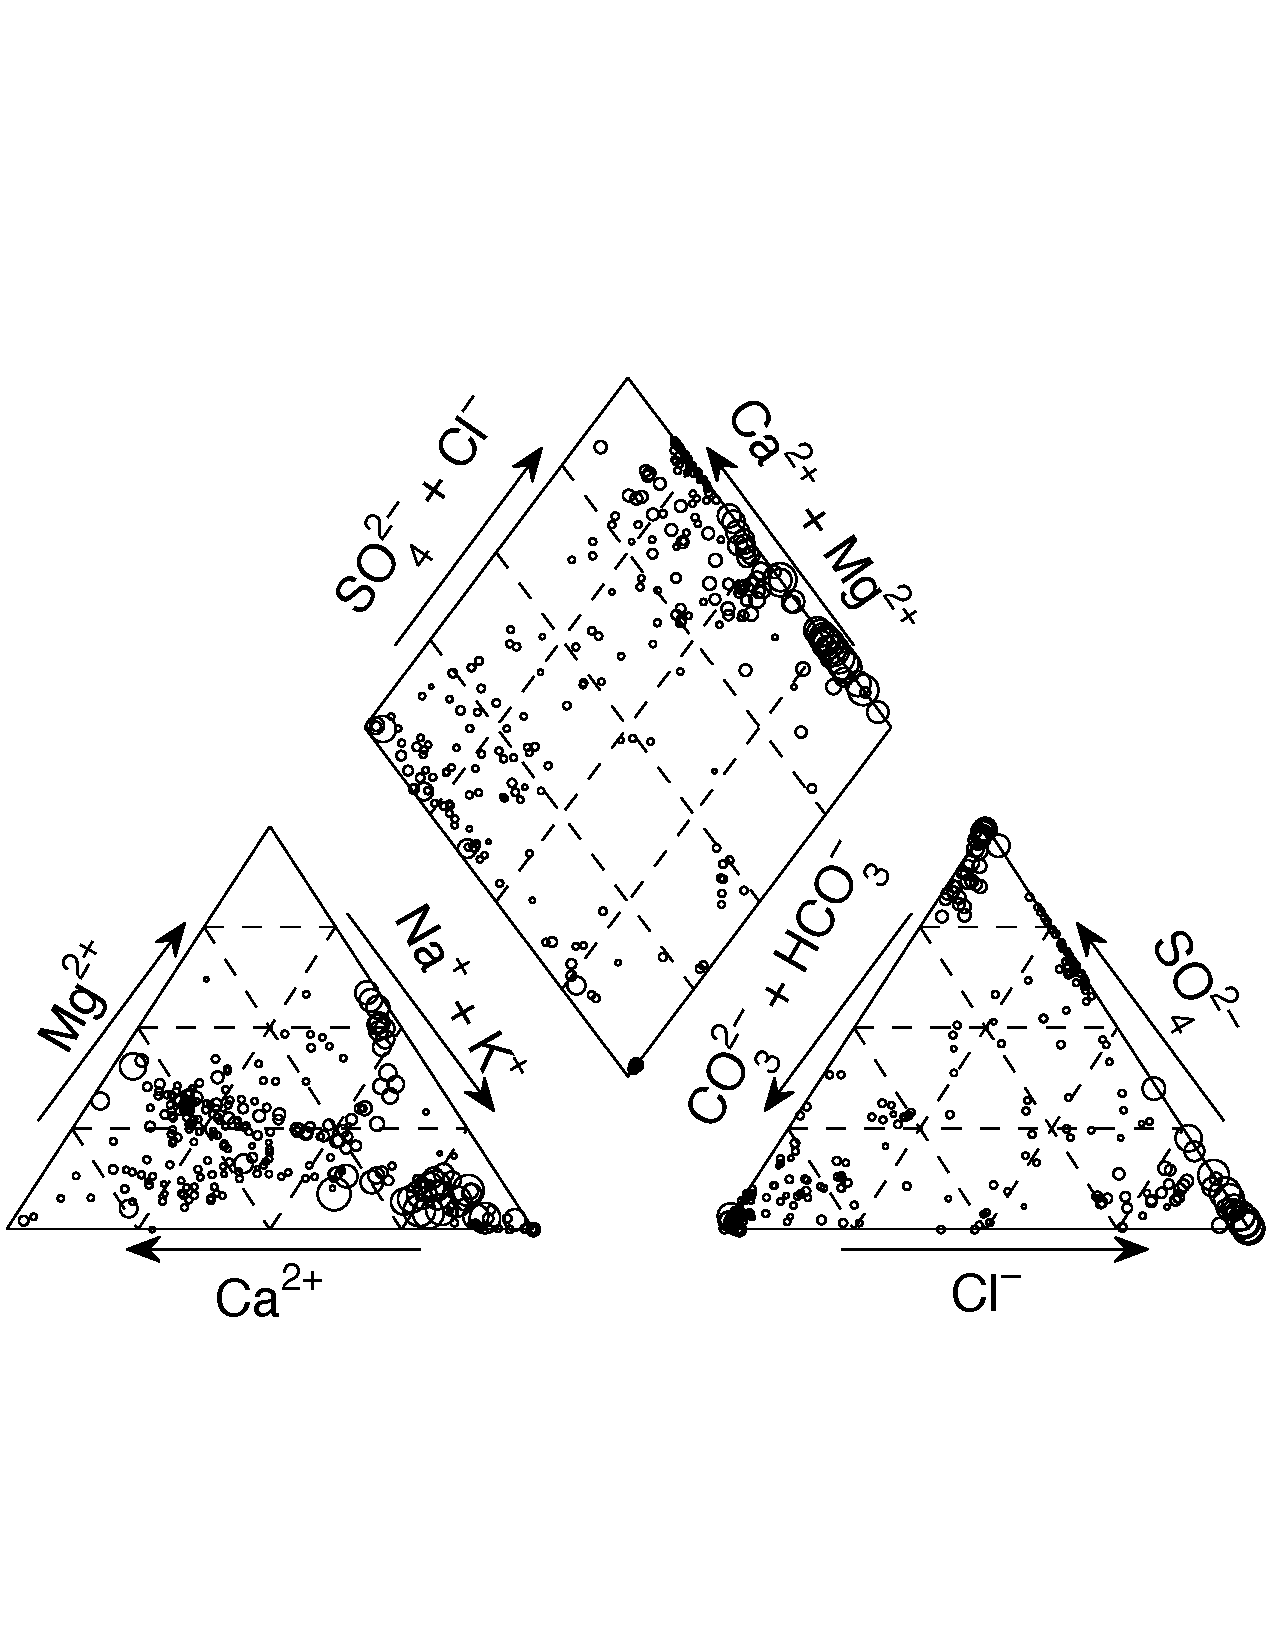
\includegraphics[width=0.67\textwidth]{Ch3_figures/GW-piper.pdf}
\caption{Piper diagram of ground water chemistry for circumneutral (5.5 $<$ pH $<$ 8.5) groundwater. Points scaled based on total dissolved solids. All plots range from 0 -- 100\%.}\label{fig:GW-chem-piper}
\end{center}
\end{figure}

Based on the available data three qualitative, rule-based water types were classified: fresh water ($N=122$; $6.5\leq$ pH $\leq8.5$; I $\leq0.1$ mol/kg), brines ($N=20$; $5.3\leq$ pH $\leq8.0$; I $\geq1.0$ mol/kg), and acidic waters ($N=63$; pH $<5.3$);
ionic strength and pH values were chosen to maximize data points within the various water classes while maintaining a reasonable bound on parameters.
Further subdivision of the freshwater data was possible (e.g. based on relative cation/anion composition) but was not pursued in favor of retaining a larger sample size.
The medians of the REE distributions of the classified groundwaters are shown in Figure~\ref{fig:GW-type-med}.

Utility of REE as tracers is reliant on identifying distinctive trends in different water types.
Of note in Figure~\ref{fig:GW-type-med} is the markedly higher concentrations of REE in acidic waters than either fresh water or brines, which supports the observations from Figure~\ref{fig:sum_vs_pH}, but also a deviation from the standard Oddo-Harkins effect pattern where Er and Yb are both less concentrated than their odd-numbered neighbors.
This effect was attributed to high degrees of censored or missing data for these elements (87\% for both Er and Yb in the acidic dataset) which leads to low-biased percentile estimates (as with Er and Yb) and large uncertainty (seen in all the HREE).
Despite showing little or no correlation with ionic strength (Figure~\ref{fig:REE-vs-major}) the REE, in particular the LREE and MREE, were more concentrated in brines than freshwater.

\begin{figure}[htbp]
\begin{center}
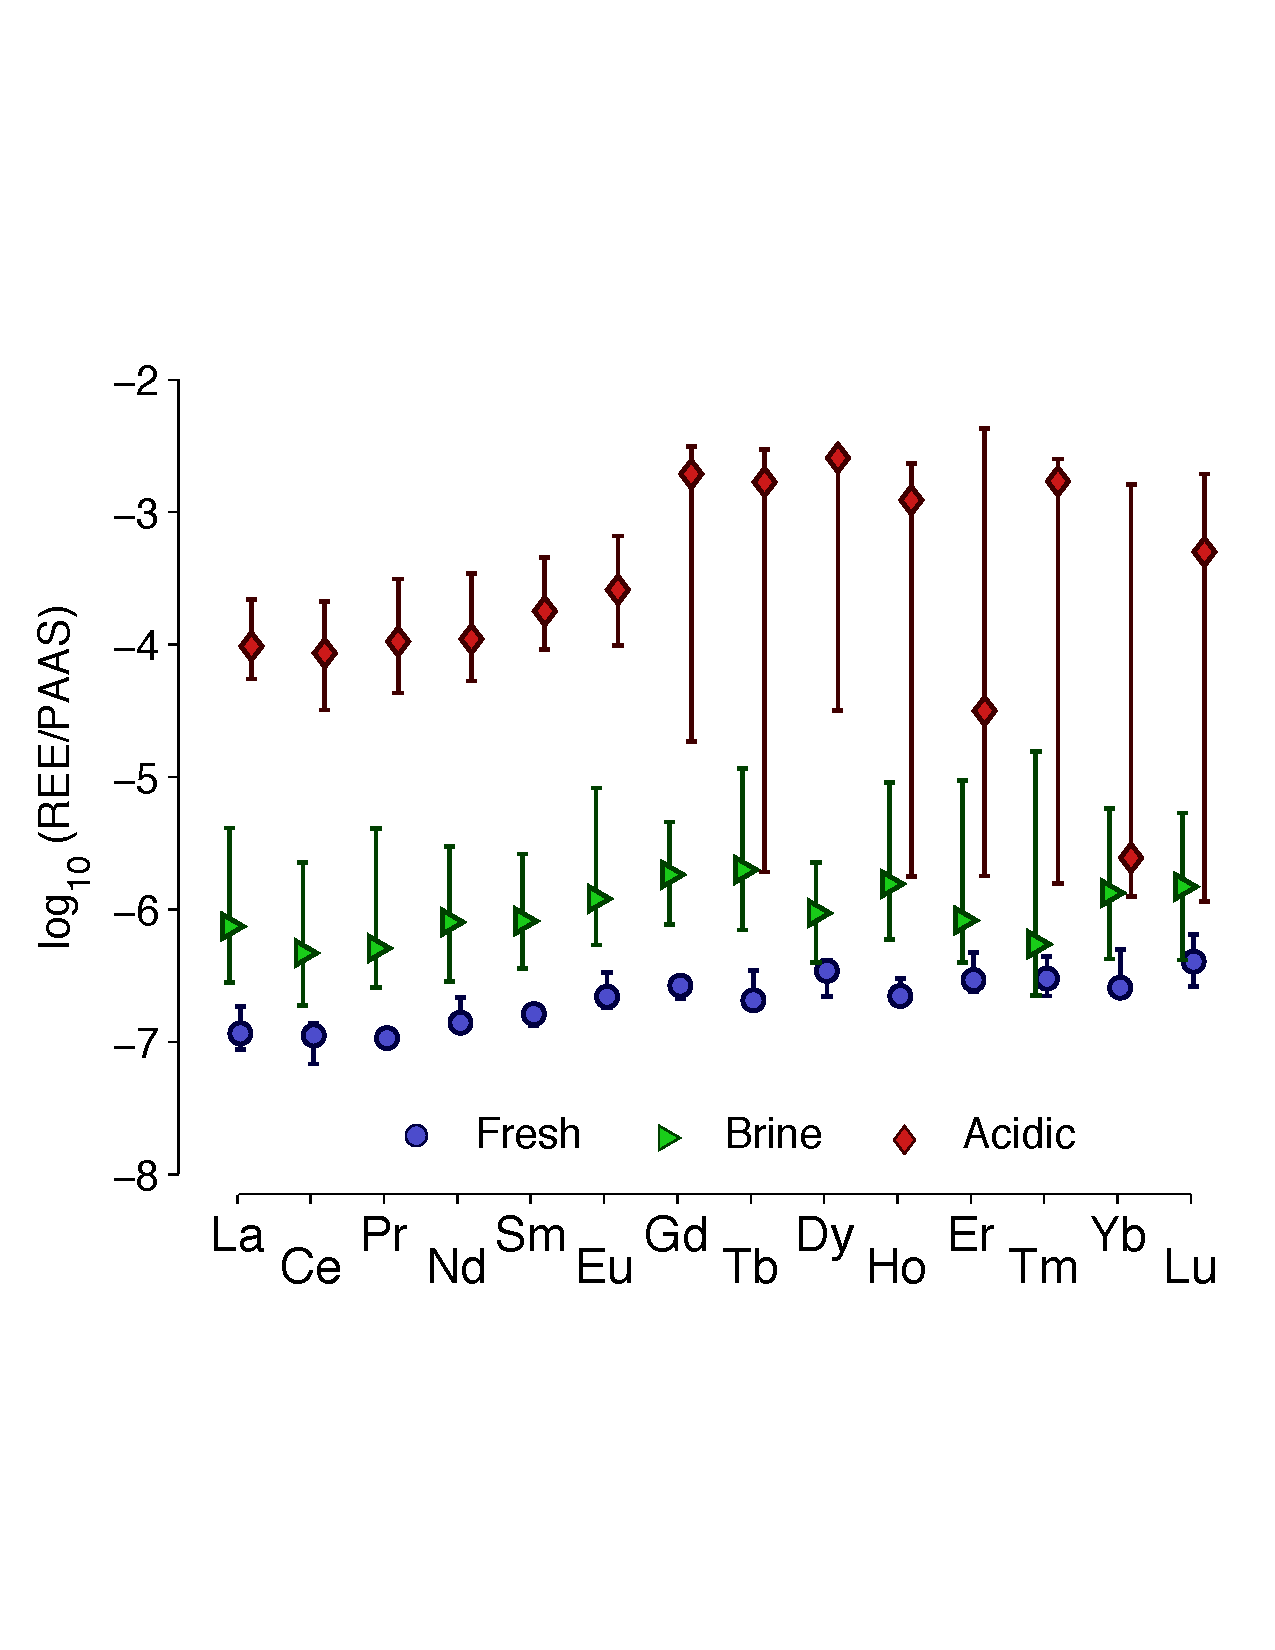
\includegraphics[width=0.67\textwidth]{Ch3_figures/REE-GW-KMmed.pdf}
\caption{Source-size weighted Kaplan-Meier estimates of median dissolved REE concentrations, normalized to Post-Archaean Average Shale (PAAS) values, in three characteristic groundwater types.
Error bars represent the 95\% confidence interval of the median.
Definitions of water classes are found in the text.
Estimates were made for individual elements, thus results do not represent a ``typical'' water sample across the REE suite.}\label{fig:GW-type-med}
\end{center}
\end{figure}

Understanding of the aqueous systematics of the REE is dominated by studies of fresh groundwaters, surface waters, and seawater.
Only 14\% of the groundwater data gathered had a calculated ionic strength of 1.0 mol/kg or greater (Figure~\ref{fig:I-ecdf}).
While thermodynamic models have been developed to predict REE aqueous speciation in brines \citep{Millero_GCA_1992},
the energetics of precipitation-dissolution and sorption-desorption in the REE system are not well defined for high ionic strength, chemically complex brines \citep{Quinn_MC_2006}.
Moreover, increased utilization of groundwater \citep{Chen_WRM_2013} in response to population growth, economic development, and climate change and the potential to exploit saline aquifers \citep{Benko_EES_2008} underscores the need to better understand the trace metal chemistry of brines.

\begin{figure}[htbp]
\begin{center}
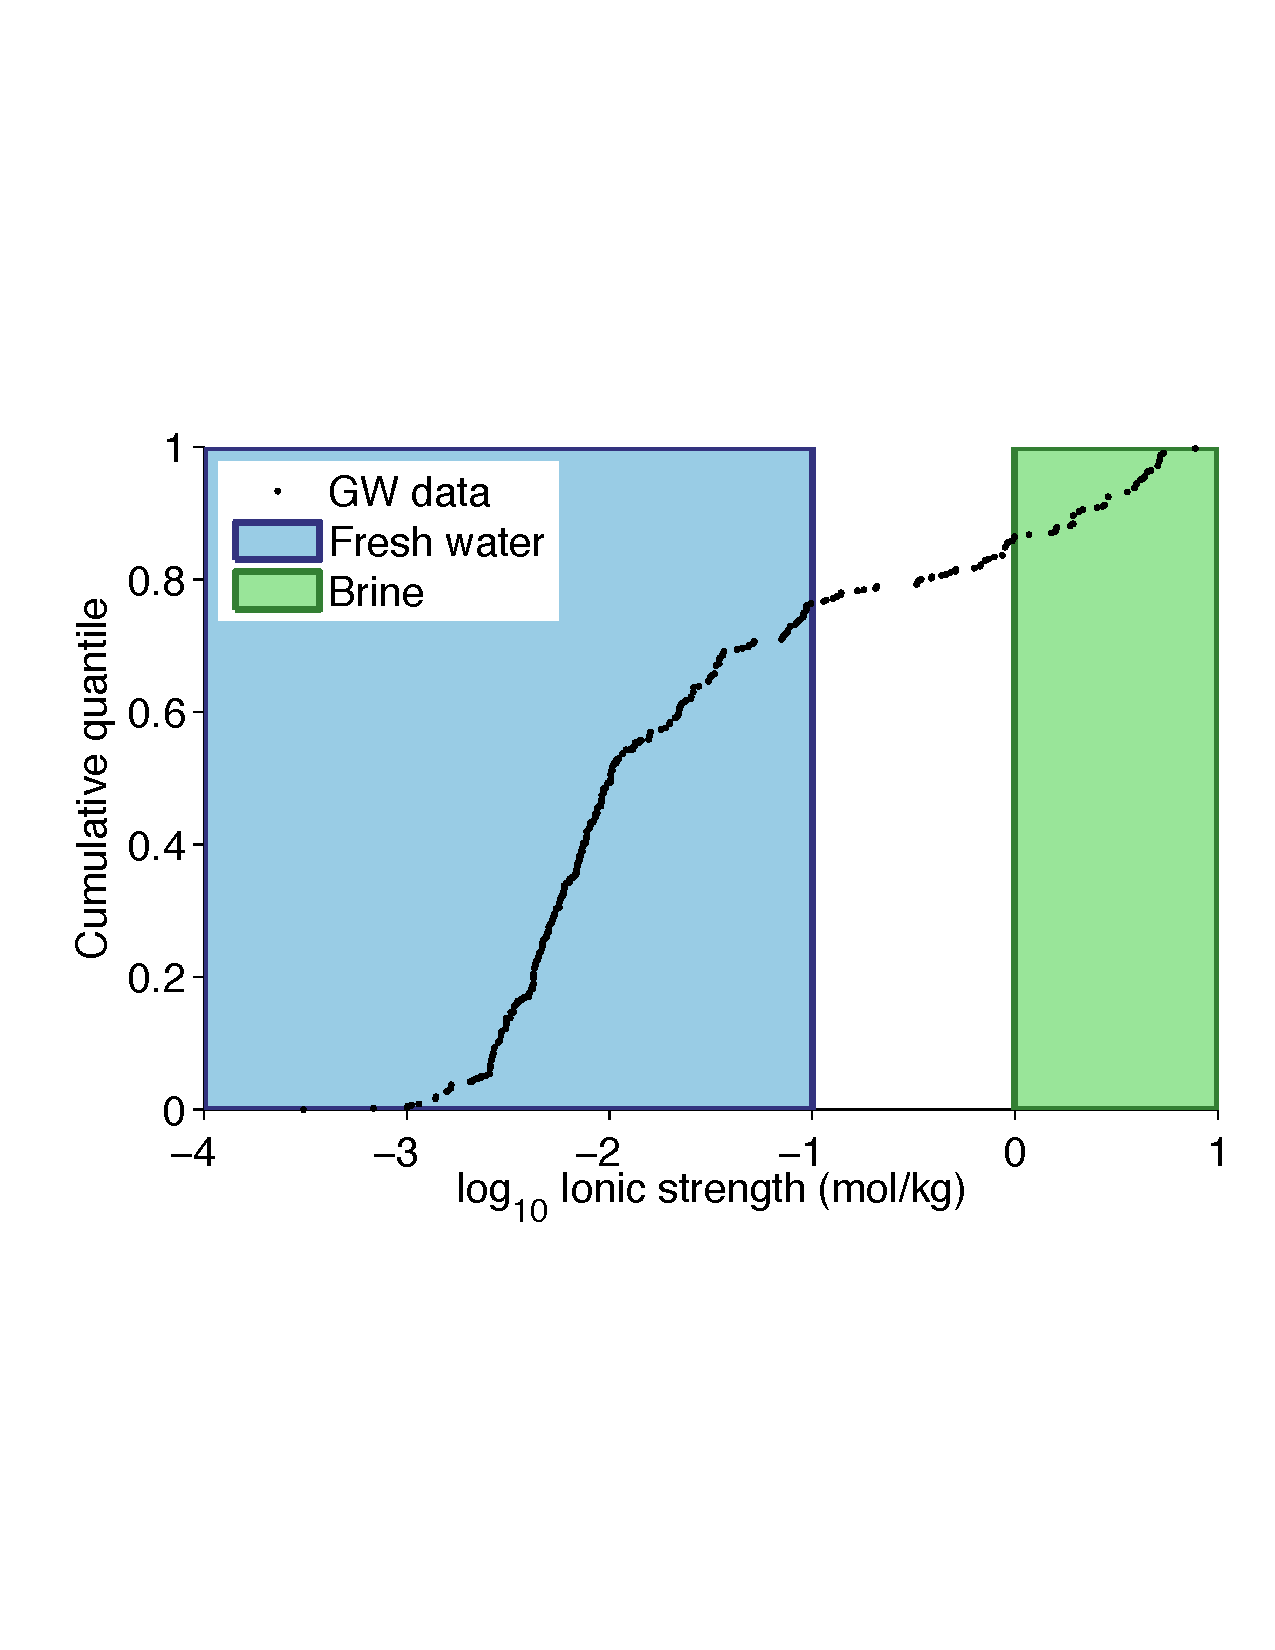
\includegraphics[width=0.67\textwidth]{Ch3_figures/GW-ionic-strength.pdf}
\caption{Source-size weighted, empirical cumulative distribution of calculated ionic strength in groundwater data set. Ionic strength calculated using PHREEQC \citep{PHREEQC}.}\label{fig:I-ecdf}
\end{center}
\end{figure}

Comparison of the HREE/MREE ratio to the MREE/LREE ratio succinctly captures the general shape of the REE profile of a sample, greatly simplifying visual comparison of samples.
Figure~\ref{fig:RDV-biplot} plots this scatter for classified groundwater data where all 14 REE were detected (39\% of the dataset).
For freshwater, more than 90\% of the samples exhibited MREE/LREE ratios greater than 1, with a median ratio of 1.74 and an IQR from 1.36 to 2.64.
HREE-MREE fractionation was more balanced with 53\% of samples having HREE/MREE ratios greater than 1, with a median ratio of 1.25 and an IQR from 0.64 to 1.6.
These data closely resemble the trends observed in the unclassified data set (not pictured), likely because freshwaters account for a large portion of the total data.
Fewer brine and acidic samples are available to plot, however brines appear to cluster with HREE enrichment, with all samples having MREE/LREE ratios greater than 1.0 and only 1 sample having HREE/MREE ratio less than 1.0, while acid samples exhibit convex-down profiles (MREE/LREE $> 1$ and HREE/MREE $< 1$).
However, it is difficult to ensure these are representative patterns given the small sample size for these water classes.

\begin{figure}[htbp]
\begin{center}
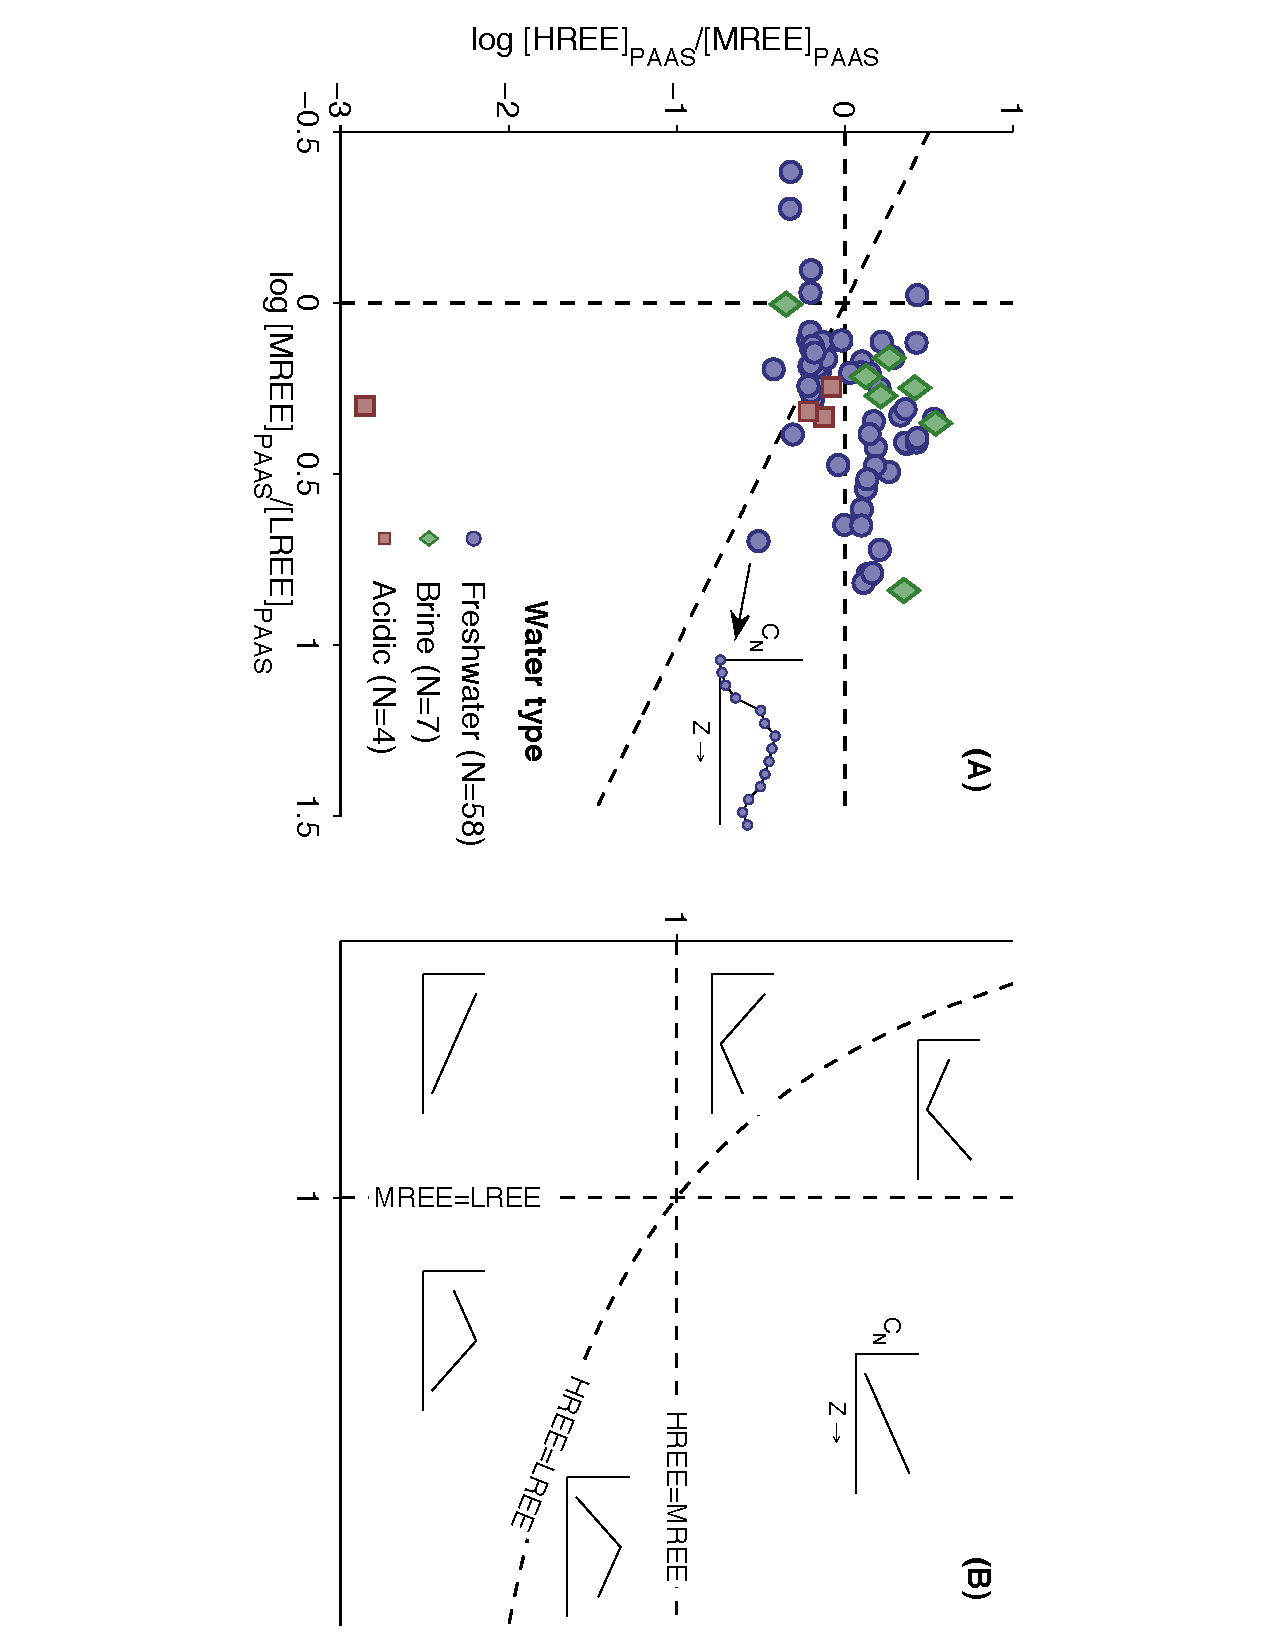
\includegraphics[width=\textwidth]{Ch3_figures/RDV-grouped-biplot.pdf}
\caption{(A) Averaged Post-Archaean Average Shale (PAAS) element ratio biplot for chemistry-classified groundwater data with no censoring, and (B) a schematic intended for interpretation, illustrating the general shape of the REE profile for a given sample.
Because each marker in (A) is a summary of the REE profile for an individual sample, an inset has been included to show the raw data (PAAS-normalized concentration, $C_N$, vs. elements in order of increasing atomic number, $Z$) for one sample.
The schematic in (B) is modified from Stolpe et al. \citep{Stolpe_GCA_2013} with permission.
Copyright 2013 Elsevier.
Note that the values in (A) have been log-transformed while the axes of the schematic are linear.}\label{fig:RDV-biplot}
\end{center}
\end{figure}

\subsection{Limitations of assembled dataset}

The primary goal of this analysis was to understand large-scale REE variability and trends.
However, researchers have understood that, because of complex geologies and watershed characteristics, there is significant merit in studying local, small-scale REE systematics.
This leads to specialized studies, for example, on the importance of colloids,33, 35, 42, 84, 87
phosphate complexation,12, 21, 91
or organic compounds.41, 85, 132-134 
While this approach yields crucial understanding of these processes, it also leads to a paucity of consistent data for inter-study comparison.
Moreover, it could motivate spurious extrapolation of thermodynamic or case study data to unique systems.

\bibliographystyle{unsrtnat}
\bibliography{Ch3_bib_edit}






\chapter{Determination of Rare Earth Elements in Hypersaline Solutions Using Low-Volume, Liquid-Liquid Extraction}\label{chap:LLE}
\chaptermark{LLE method for brines}

This chapter is adapted from a publication by the same name, co-authored by David A. Dzombak and Athanasios K. Karamalidis.
This paper is citable as: 

Noack, C. W.; Dzombak, D. A.; Karamalidis, A. K., Determination of Rare Earth Elements in Hypersaline Solutions Using Low-Volume, Liquid-Liquid Extraction. \textit{Environ. Sci. Technol.} \textbf{2015}, \textit{Article ASAP}, DOI: 10.1021/acs.est.5b00151

My contributions to this work were the experimental design; execution of experiments including ICP-MS analysis; data analysis and visualization; interpretation of results; and drafting of the manuscript.

\clearpage

\section*{Abstract}
Complex, hypersaline brines --- including those co-produced with oil and gas, rejected from desalination technologies, or used as working fluids for geothermal electricity generation --- could contain critical materials such as the rare earth elements (REE) in valuable concentrations.
Accurate quantitation of these analytes in complex, aqueous matrices is necessary for evaluation and implementation of systems aimed at recovering those critical materials.
However, most analytical methods for measuring trace metals have not been validated for highly saline and/or chemically complex brines.
Here we modified and optimized previously published liquid-liquid extraction (LLE) techniques [Shabani et al., \textit{Anal. Chem.} 1990, 62 (24) 2709-2714; Lawrence and Kamber, \textit{Geostand. Geoanal. Res.} 2007, 31 (2) 95-103], using bis(2-ethylhexyl) phosphate as the extractant in a heptane diluent, and studied its efficacy for REE recovery as a function of three primary variables: background salinity (as NaCl), concentration of a competing species (here Fe), and concentration of dissolved organic carbon (DOC).
Results showed that the modified LLE was robust to a range of salinity, Fe, and DOC concentrations studied as well as constant, elevated Ba concentrations.
With proper characterization of the natural samples of interest, this method could be deployed for accurate analysis of REE in small volumes of hyper-saline and chemically complex brines.

\section{Introduction}

The rare earth elements (REE) are among the most frequently cited critical materials for clean energy and high-tech manufacturing \citep{APS_CritMat,USDOE_CritMat}.
The unique and varied properties of REE have led to their application in more consumer products than nearly any other element group \citep{Castor_Hedrick}.
REE are mostly obtained from mining and processing of REE-enriched ores \citep{USDOE_CritMat}.
While economically preferred, mining is laborious with a significant environmental burden, and inexpensive alternative sources of critical materials are sought after resources.

Aqueous byproduct or waste streams, both natural and industrial, are potential sources of the REE and other critical materials.
With increasing global interest in geothermal energy \citep{Lund_Geothermics_2011},
development of unconventional oil and gas resources (e.g. hydraulic fracturing of organic rich shales) \citep{EIA_2013},
and desalination technologies \citep{Shannon_Nat_2008, Elimelech_Sci_2011},
large volumes of waste brines are being managed and processed at great expense.
Development of technologies for recovery of valuable byproducts, such as the REE, from these waste streams could improve the economics of these technologies while diversifying available critical material resources.
Development of such technologies requires accurate determination of the source REE concentration in order to develop and implement recovery systems.
However, precise quantitation of REE in complex matrices like brines is a significant challenge for conventional instrumentation such as inductively coupled plasma mass spectrometry (ICP-MS) \citep{Agatemor_ACA_2011}.

There exists a dearth of methodologies in the analytical literature for quantitation of REE in brines by ICP-MS.
Many approaches have been applied for separation and concentration of REE from aqueous media including solid-phase extraction (SPE)
\citep{Benkhedda_JAAS_2001, Fu_Tal_2007, Haley_MC_2003, Halicz_JAAS_1996, Hirata_Tal_2002, Kajiya_SAB_2004, Katarina_Tal_2009, Kim_AG_2010, Kuhn_FJAC_2000, Kumar_Desal_2011, Moller_SAB_1992, Stetzenbach_GW_1994, Vicente_SAB_1998, Wen_Analyst_1999, Willie_SAB_2001, Zhang_AC_1998, Zhu_Tal_2009},
co-precipitation (co-ppt) \citep{Shaw_AC_2003, Shannon_REEinGWFS, Raso_Tal_2013},
and liquid-liquid extraction (LLE) \citep{Shabani_AC_1990, Lawrence_GGR_2007, Kimura_BCSJ_1960, Kimura_BCSJ_1961}.
However, nearly all studies in the analytical chemistry literature have focused on fresh water or seawater matrices, neglecting hypersaline waters (i.e. more concentrated than $\sim0.7$ M NaCl or seawater).
Despite this deficiency, approximately 14\% of published measurements of REE in groundwater constitute brine samples (greater than 1 eq/kg ionic strength) \citep{Noack_EST_2014}, with these analyses utilizing methodologies not explicitly validated for extreme salinity.

Commonly applied separation techniques such as SPE and co-ppt may lack the robustness necessary to analyze REE in hypersaline brines.
For example, high dissolved organic carbon may lead to fouling of column-based SPE while high dissolved metal loads may lead to saturation of the surface sites responsible for REE binding.
Oliveira et al. \citep{Oliveira_JAAS_2011} ascribed diminished Zn recovery in 166\textperthousand\ salinity produced water to competitive sorption of matrix cations on their iminodiacetate resin.
Similarly, excessive cations in hypersaline solutions may screen the REE from sorption sites during co-ppt, a phenomenon noted by Nelson et al. \citep{Nelson_ESTL_2014} for Ra determination in produced waters from the Marcellus Shale by both \ce{BaSO4} and \ce{MnO2} co-ppt.
Moreover, at the elevated pH necessary for SPE and co-ppt techniques, the formation of energetically favorable, neutral- or negatively-charged aqueous complexes of the REE (with both organic and inorganic ligands) can further limit REE-particle partitioning \citep{Erel_GCA_1993}. 

Liquid-liquid extractions are potentially robust to all of these conditions and represent an attractive alternative for REE separation from hypersaline solutions \citep{Nash_SXIX_1993}.
Since LLE of REE from highly acidic solutions has been thoroughly studied for separation of lanthanides and actinides during nuclear fuel reprocessing \citep[e.g. refs.][]{Weaver_ORNL_1964, Nilsson_SXIX_2007} elevated pH is not required of LLE techniques.
Moreover, electrolyte theory dictates that increased sample salinity should enhance chemical partitioning (through salting out of neutral/micellar REE-organic ligand complexes from the aqueous feed to the organic solvent) and physical phase separation (by collapsing the electric double layer of the organic droplets, hastening coalescence).
A primary obstacle in extraction of hydrophilic metals to a hydrophobic, organic phase is the dehydration of the metal cations in the aqueous phase.
However, increasing salt concentrations decrease the effective concentration of water in the solution available for hydration of the target metal cations (REE), improving the energetics of the extraction \citep{Nash_SXIX_1993}.

In this work, efficiency of REE separation and concentration from synthetic brines using a LLE method for quantitative analysis was studied.
The LLE method was adapted, modified, and optimized from previously published studies \citep{Shabani_AC_1990, Lawrence_GGR_2007}.
For the LLE, a common ligand used for REE complexation and extraction, bis(2-ethylhexyl) phosphate (HDEHP), was studied in a heptane diluent.
The objectives of this work were to: (1) evaluate the feasibility of REE recovery from small volumes of hypersaline solutions by LLE, (2) optimize the LLE methodology for high salinity brines, and (3) study the influence of brine composition on REE recovery.

\section{Modified liquid-liquid extraction procedure}

The modified LLE method adheres to many of the physical steps of the methods originally developed by Shabani et al. 
\citep{Shabani_AC_1990} and Lawrence and Kamber \citep{Lawrence_GGR_2007}, but following optimization, differs in the operating conditions.
A schematic flowsheet of the process is shown in Figure~\ref{fig:flowsheet}.
The process involved sample preparation, followed by three cycles of extraction, whereby the REE were complexed by the HDEHP ligand and brought into the organic phase, leaving an REE-free, waste brine.
Matrix elements were rinsed from the organic phase with dilute acid, and, finally, the REE were recovered by four cycles of elution with strong acid.
This REE-loaded aqueous phase was then analyzed by ICP-MS.
The details of the process are described in following. Details of sample preparation, instrumentation, analytical protocols, and data analysis methods are presented in Section~\ref{sec:MnM}.

\begin{sidewaysfigure}[htbp]
\begin{center}
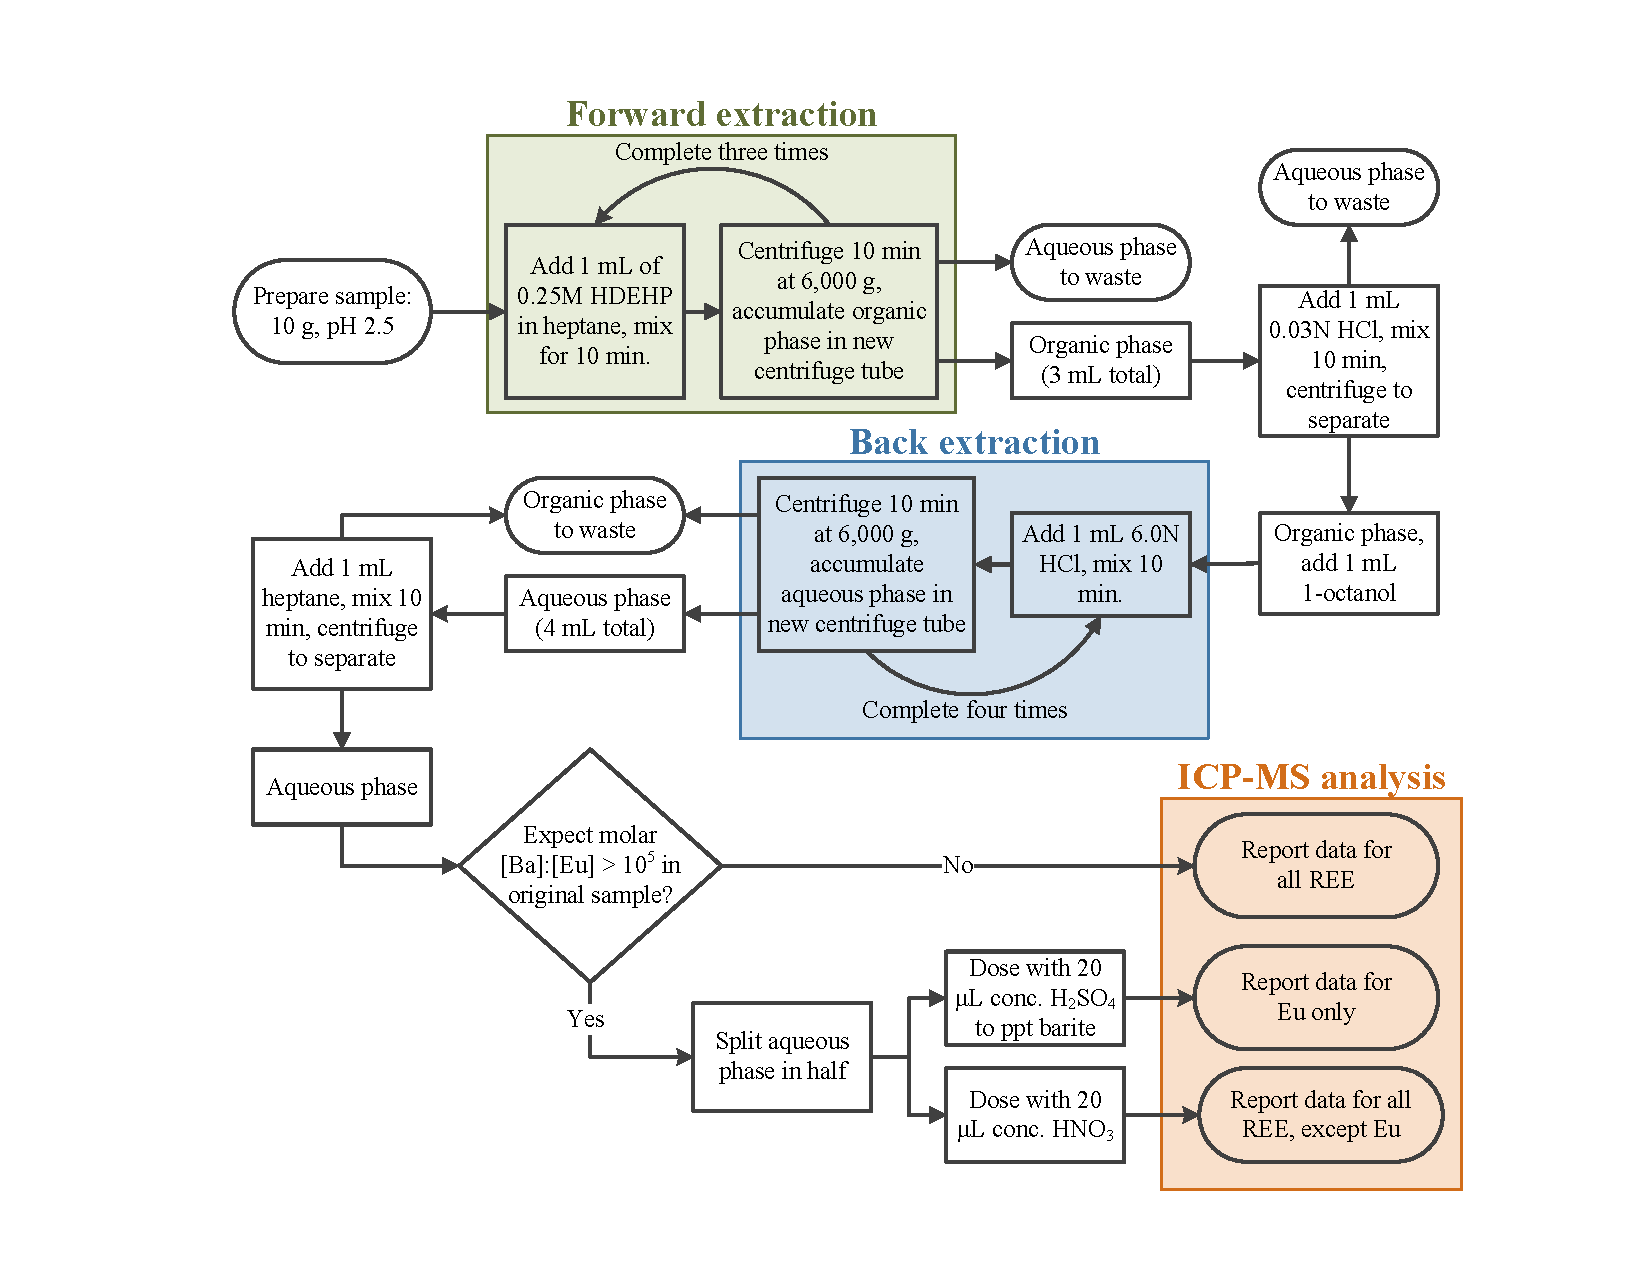
\includegraphics[width=0.8\textwidth]{Ch4_figures/LLE-flowsheet.pdf}
\caption{Liquid-liquid extraction method flowsheet for separation and concentration of REE from small volume, hypersaline brines. The decision node for the [Ba]:[Eu] molar ratio assumes a \ce{BaO+} formation rate on the order of 0.1\% in the ICP-MS.}\label{fig:flowsheet}
\end{center}
\end{sidewaysfigure}

Synthetic brine solutions were adjusted to pH 2.5 in 50 mL PP centrifuge tubes with \ce{HNO3} and subsequently split into 10 g aliquots in 15 mL PP centrifuge tubes for replicate experiments.
For each aliquot or sample, the process for REE extraction and recovery is as follows.
One (1) mL of 0.25 M HDEHP in heptane was added to the aqueous solution.
HDEHP was used as complexing agent for REE.
The phases were emulsified and mixed end over end for 10 minutes.
The phases were separated by centrifugation at 6,000$\times$g for 10 minutes and the light organic phase was removed from the centrifuge tube via pipette and accumulated in a new centrifuge tube, retaining the aqueous phase in the original tube.
This process, whereby the REE are complexed with HDEHP and partitioned into the heptane (termed forward extraction), was completed a total of three times.
Following the third forward extraction, the aqueous phase was discarded.

To remove any matrix (Na, Fe, etc.) and interfering species (i.e. Ba) that partitioned during forward extraction, the accumulated organic phase (3 mL total) was rinsed with 1 mL of pH 1.5 HCl.
This mixture was emulsified and separated by the same methods as the forward extraction.
Once separated, the dense aqueous phase was removed via pipette and discarded.

A concentrated acid solution was used to dissociate the REE-HDEHP complexes and return the REE to an aqueous phase (termed back extraction).
To decrease the REE-HDEHP complexation strength and encourage complete recovery \citep{Shabani_AC_1990},
1 mL of 1-octanol was added to the organic phase.
Back extraction was achieved with four, sequential steps of stripping with 1 mL of 6.0 N HCl (collecting the eluted REE in a total of 4 mL acid).
As with the forward extraction, the sample was emulsified and mixed end over end for 10 minutes and then separated via centrifugation at 6,000$\times$g for 10 minutes.
After centrifugation the aqueous phase was removed via pipette and accumulated in a separate centrifuge tube, retaining the organic phase in the original tube.
Following the four back-extractions, the organic phase was discarded.

The collected acid volume (4 mL) was then rinsed with 1 mL of heptane to remove any dissolved organics from the aqueous phase.
Phase mixing and separation were accomplished in the same manner as all other steps.
Following centrifugation, the dense aqueous phase was removed and analyzed.

Preliminary experiments (Figure~\ref{fig:Ba-removal}) indicated that, while Ba was successfully removed in the course of the LLE ($>99.9\%$ average reduction) and the HEHe-mode collision cell in the ICP-MS was successfully limiting \ce{^{135}Ba^{16}O+} interferences with \ce{^{151}Eu+} (\ce{^{135}Ba^{16}O+}:\ce{^{135}Ba+} $\sim0.2\%$ on average), initial Ba concentrations were so high that ppb level, background Eu concentrations were observed (Figure~\ref{fig:REE-bkgd}).
Thus, in order to determine Eu accurately in these synthetic brines an additional step was tested, where an aliquot of the final, collected acid volume was dosed with 20 \si{\uL} concentrated sulfuric acid (\ce{H2SO4}) to precipitate any remaining barium as barite (\ce{BaSO4}).
Efficiency of Ba removal after \ce{H2SO4} addition is compared in Figure~\ref{fig:Ba-removal}B and \ref{fig:Ba-removal}D.
It should be noted that this step was unnecessary for samples without Ba.

The methodology of Jenner et al. \citep{Jenner_CG_1990} as modified by McGinnis et al. \citep{McGinnis_GN_1997} was employed to correct for matrix effects, isobaric interferences, and instrument drift during ICP-MS analysis.
For each sample a 2 mL aliquot was spiked with 2 mL of a mixed element standard (5\% \ce{HNO3} background) while a separate 2 mL aliquot was diluted with 2 mL of blank 5\% \ce{HNO3}.
These solutions were analyzed sequentially to examine sample-specific matrix effects and were followed by a 5\% \ce{HNO3} flush.
At the beginning of each analysis run and after every third sample, two separate standard solutions and an analytical blank were analyzed to monitor instrument drift and isobaric, polyatomic interferences (e.g. \ce{^{135}Ba^{16}O+} on \ce{^{151}Eu+} and light REE-oxides on heavy REE).
Eight, serially-diluted, multi-element standard solutions ranging in concentration from 50 ppt to 100 ppb were analyzed at the beginning and end of each run to confirm the linearity assumed by the internal/external calibration.
Typical analytical uncertainty was between 3 and 5\%.
Because of high backgrounds of Gd in our laboratory and high Ba in the experiments, oxide corrections for \ce{^{137}Ba^{16}O+} interference on \ce{^{151}Eu+} and \ce{^{157}Gd^{16}O+} on \ce{^{173}Yb+} were applied as in Aries et al. \citep{Aries_GN_2000} after ICP-MS analysis.

\section{Materials and methods}\label{sec:MnM}

\subsection{Chemicals and equipment}

For the LLE, n-heptane (Chromasolv\textsuperscript{\textregistered}; Lot \# SHBC0837V),
 1-octanol (Chromasolv\textsuperscript{\textregistered}; Lot \# SHBC6245V),
 and HDEHP (99.7\% purity; Lot \# MKBK0176V) were acquired from Sigma Aldrich.
 Nitric acid (\ce{HNO3}; BDH ARISTAR\textsuperscript{\textregistered} Plus, VWR; assay 69 wt.\%; Lot \# 1113050) was used for sample pH adjustment and as the solvent for all analyses.
 Hydrochloric acid (HCl; BDH ARISTAR\textsuperscript{\textregistered} Plus, VWR; 35 wt.\%; Lot \# 4113083) was used for matrix rinsing and REE back-extraction in the LLE.
 Chloride salts of Na (Sigma Aldrich; $\geq99\%$ purity), Ba (Alfa Aesar; $\geq 99.998\%$ purity), and Fe (Sigma Aldrich; $\geq 99.9\%$ purity, trace metal basis) and valeric acid (Alfa Aesar; 99\% purity) were used for preparation of synthetic brines.
 Single element standard solutions (1000 \si{\ug}/L) of the REE and all elements necessary for internal and external standardization were obtained from Inorganic Ventures.
 Polypropylene (PP) centrifuge tubes were used in the LLE and glass volumetric flasks were used to prepare organic phases.
Ultrapure water (ASTM Type I, 18.2 \si{M\ohm}/cm) was used for sample preparation and was prepared using a Barnstead NANOpure\textsuperscript{\textregistered} water purification system.
An OrionTM 8165BNWP ROSSTM Sure-FlowTM pH electrode (Thermo Scientific), coupled to an accumetTM XL600 meter (Fisher Scientific), was used for pH measurements of high-total dissolved solid (TDS) solutions.
The pH meter was calibrated with pH 2.0, 4.0, and 7.0 standards daily.
All samples were prepared gravimetrically using an analytical balance with 0.01 mg precision (Adam Equipment).

All analyses were performed on an Agilent 7700x ICP-MS with HEHe-mode octopole reaction cell.
Operating parameters were optimized daily via the auto-tune function of the Agilent MassHunter software using 1000:1 diluted Agilent tuning solutions;
typical operating parameters and monitored analyte masses are given in Table~\ref{tab:ICPMS}.

\begin{table}[htdp]
\caption{Typical operating conditions for ICP-MS analysis.
Analysis performed on Agilent 7700x using oxygen-free argon as the carrier and dilution gas and ultra high-purity helium in the reaction cell.
Conditions determined using 1000:1 diluted Agilent tuning solution.
For elements where multiple mass-to-charge ratios were monitored, \ce{^{148}Sm}, \ce{^{151}Eu}, and \ce{^{157}Gd} were used in data analysis.}\label{tab:ICPMS}
\begin{center}
\begin{tabular}{l l l}
\hline
 & Parameter & Value \\ \hline
 Plasma & & \\
  & RF power & 1600 W \\ 
  & Nebulizer pump rate & 0.10 rps \\
  & Carrier argon flow rate & 0.61 L/min \\ 
  & Dilution argon flow rate & 0.36 L/min \\ 
 Lenses & & \\ 
  & Extract 1 & 0.0 V \\
  & Extract 2 & -200.0 V \\
  & Omega bias & -110 V \\
  & Omega lens & 9.6 V \\
  & Cell entrance & -110 V \\
  & Cell exit & -150 V \\
  & Deflect & -74.8 V \\
  & Plate bias & -150 V \\
 Octopole reaction cell & & \\
  & Octopole bias & -100.0 V \\
  & Octopole RF & 200 V \\
  & He flow rate & 10 mL/min \\
  & Energy discrimination & 7.0 V \\
 Data aquisition & & \\
  & Replicates & 5 \\ 
  & Integration time & 0.3 s\\
 Masses monitored & & \\  
  & \multicolumn{2}{l}{\ce{^{45}Sc}, \ce{^{89}Y}, \ce{^{115}In}, \ce{^{135}Ba}, \ce{^{137}Ba}, \ce{^{139}La}, \ce{^{140}Ce},} \\ 
  & \multicolumn{2}{l}{\ce{^{141}Pr}, \ce{^{145}Nd}, \ce{^{147}Sm}, \ce{^{148}Sm}, \ce{^{151}Eu}, \ce{^{153}Eu},} \\ 
  & \multicolumn{2}{l}{\ce{^{157}Gd}, \ce{^{158}Gd}, \ce{^{159}Tb}, \ce{^{163}Dy}, \ce{^{165}Ho}, \ce{^{167}Er},} \\
  & \multicolumn{2}{l}{\ce{^{169}Tm}, \ce{^{173}Yb}, \ce{^{175}Lu}} \\
 Oxides and doubly charged & & \\  
  & \multicolumn{2}{l}{\ce{^{140}Ce^{16}O+}/\ce{^{140}Ce} $< 2.1\%$} \\ 
  & \multicolumn{2}{l}{\ce{^{140}Ce^2+}/\ce{^{140}Ce} $< 1.6\%$} \\ \hline
\end{tabular}
\end{center}
\label{default}
\end{table}%

\subsection{Recovery analysis by surrogate recovery}

In the absence of a high-salinity, certified reference material for REE, the IUPAC recommended methodology of surrogate recovery \citep{IUPAC} was used to study the recovery of REE by this LLE method.
Synthetic brine samples were either left blank or spiked with constant amounts of REE.
The difference in results between these samples yielded the mass of the spiked analytes recovered by the LLE method.
Additionally, indium was included in the spike solution as it is commonly employed as an internal standard for REE separation to monitor recovery \citep{Shabani_AC_1990,Zawisza_JAAS_2011}.
Data below the instrument detection limit (DL) were assigned a value of $0.5\times$DL for computation; this occurred for roughly 41\% of all the REE in the unspiked samples and 4\% in the spiked samples.

\subsection{Preparation of synthetic brines}

In addition to optimization of operating parameters, the methodology must be validated for complex brine solutions.
The complexity of the brine is a function of background salinity and interfering compounds (both inorganic and organic).
This was investigated in two stages.
First, simple solutions (1 m and 5 m NaCl) were used to evaluate feasibility.
Second, compositional complexity was explored via a uniform shell, or Doehlert, experimental design \citep{Doehlert}, varying NaCl, Fe, and dissolved organic carbon (DOC) concentrations.

The concentrations of background salinity and interfering compounds were chosen to match reported value ranges found in studies of produced waters from unconventional gas development in the Marcellus Shale \citep{Haluszczak_AG_2013, Barbot_EST_2013, Gregory_Elements_2011, Arvind_EST_2013, Vidic_Sci_2013},
however the range of compositions studied is similar to other deep, basinal brines \citep{Kharaka_REG_2000}.
Dissolved organic carbon was modeled with pentanoic (or valeric) acid, a common component of deep, saline brines \citep{Kharaka_REG_2000},
with representative metal-complexing functionality.
Additionally, organic acids have been shown to be a significant component of DOC in produced waters from the Marcellus Shale \citep{Wolford_PSU_2011}.
The parameters of interest --- concentrations of NaCl, Fe, and DOC --- were scaled linearly.
Experimental conditions for variability in salinity, Fe concentration, and DOC concentration are given in Table~\ref{tab:Doehlert}.
For all experiments the concentration of each REE (along with indium) was set at 500 ppt (parts per trillion), a value that falls between the 45th percentile (for Tm) and the 1st percentile (for La) of natural REE distributions in groundwater \citep{Noack_EST_2014}.
Total dissolved Ba was held constant at 2,000 ppm, roughly the average concentration observed by Barbot, et al. \citep{Barbot_EST_2013} for Marcellus Shale produced waters.
Results of these experiments were analyzed by multiple linear regression (MLR) to determine which parameters of the synthetic brine influenced the recovery most strongly.

\begin{table}[htdp]
\caption{Doehlert experimental design matrix for LLE validation in chemically complex brines.
Doehlert coding for each experiment are given in parentheses next to the parameter value.
All variables were varied arithmetically.} \label{tab:Doehlert}
\begin{center}
\begin{tabular}{cccc}
\hline
Exp. & [NaCl] (m) & [Fe] (ppm) & [DOC] (ppm-C) \\ \hline
1 & 2 (0) & 40 (0) & 200 (0) \\ 
2 & 3.5 (1) & 40 (0) & 200 (0) \\ 
3 & 2.75 (0.5) & 74.6 (0.866) & 200 (0) \\ 
4 & 2.75 (0.5) & 51.6 (0.289) & 363 (0.817) \\ 
5 & 0.5 (-1) & 40 (0) & 200 (0) \\ 
6 & 1.25 (-0.5) & 5.4 (-0.866) & 200 (0) \\ 
7 & 1.25 (-0.5) & 28.4 (-0.289) & 37 (-0.817) \\  
8 & 2.75 (0.5) & 5.4 (-0.866) & 200 (0) \\ 
9 & 2.75 (0.5) & 28.4 (-0.289) & 37 (-0.817) \\ 
10 & 1.25 (-0.5) & 74.6 (0.866) & 200 (0) \\ 
11 & 2 (0) & 63.1 (0.577) & 37 (-0.817) \\ 
12 & 1.25 (-0.5) & 51.6 (0.289) & 363 (0.817) \\ 
13 & 2 (0) & 16.9 (-0.577) & 363 (0.817) \\ \hline
\end{tabular}
\end{center}
\label{default}
\end{table}%

\subsection{Optimization of liquid-liquid operation parameters}

Preliminary experiments utilizing LLE conditions described by Shabani et al. \citep{Shabani_AC_1990} and Lawrence and Kamber \citep{Lawrence_GGR_2007} were unable to achieve high or consistent recovery of the REE (Figure~\ref{fig:reproduction}A,B).
These experiments showed recovery $<80\%$ for all elements in all replicates, with significant variability, as well as preferential recovery of the MREE over the L- and HREE.
It should be noted that both Shabani et al. \citep{Shabani_AC_1990} and Lawrence and Kamber \citep{Lawrence_GGR_2007} employed a mixture of mono- and di-ester phosphonic acids as the chelating ligand.
This ligand combination was also explored, however preliminary experiments provided poor results compared to the pure diester (HDEHP) under the same conditions and was not studied further.

\begin{figure}[htbp]
\begin{center}
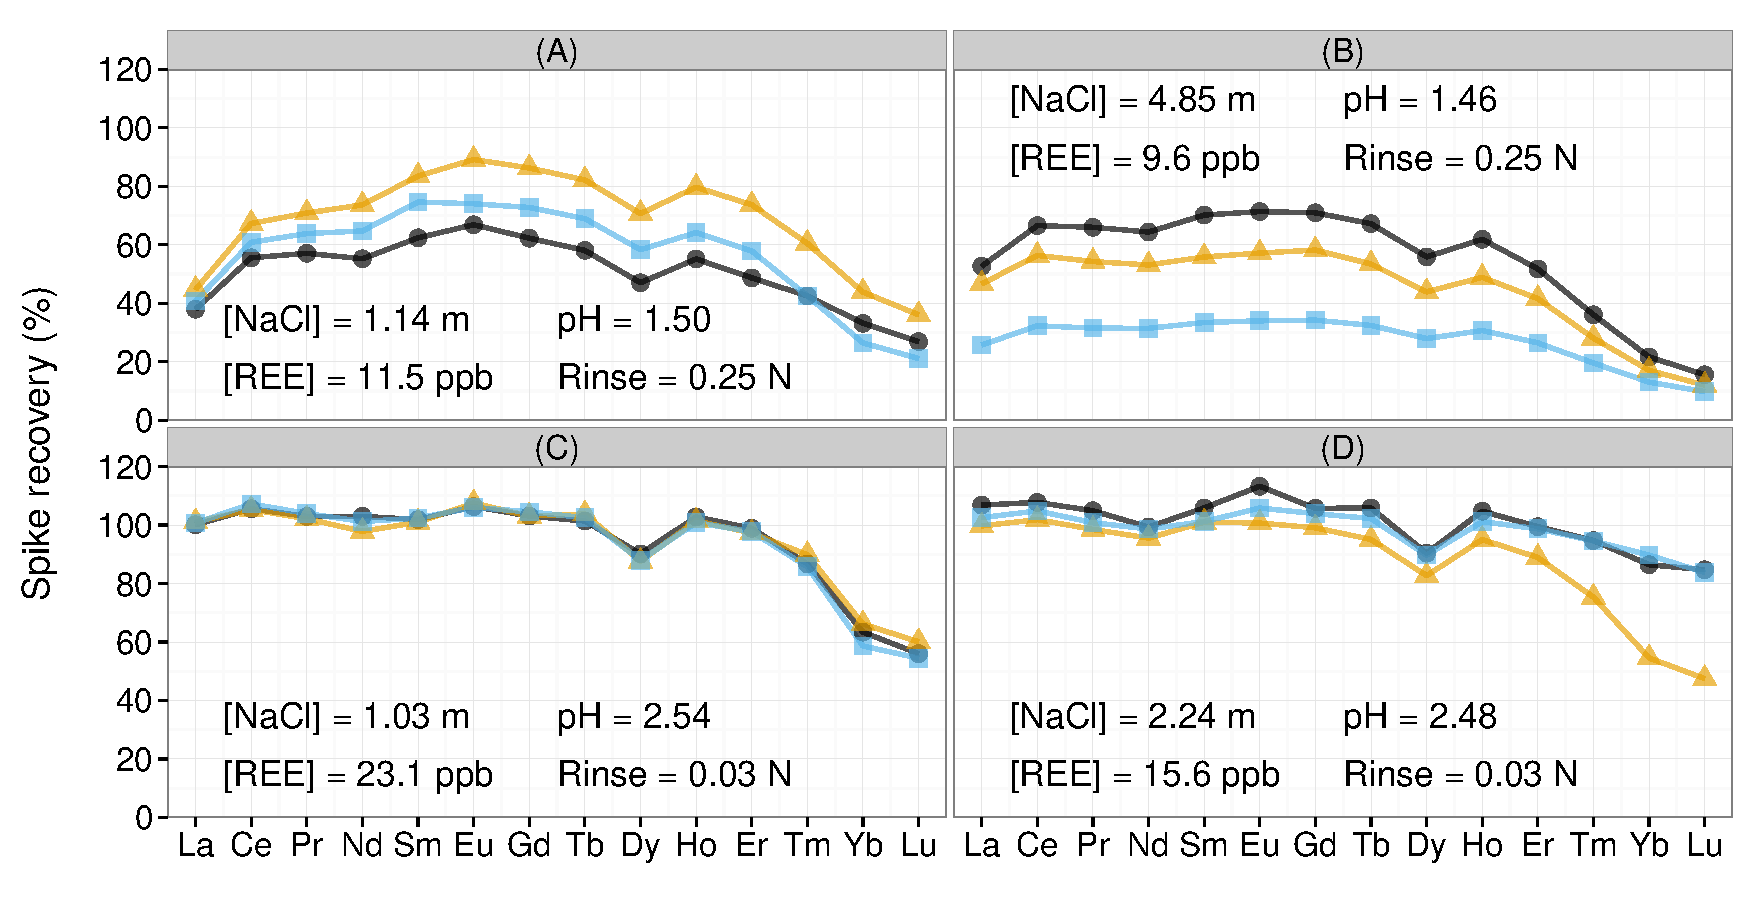
\includegraphics[width=\textwidth]{Ch4_figures/LLE-reproduction-recoveries.pdf}
\caption{REE recovery from 10 g samples of synthetic brine solutions using LLE conditions recommended by Shabani, et al.7 (A, B)
and ``optimal'' conditions predicted by multiple linear regression (C, D).
Each experiment was performed in triplicate (separate colors/shapes of plot) and the experimental conditions are shown in the subfigures.}\label{fig:reproduction}
\label{default}
\end{center}
\end{figure}

In order to optimize method performance, a linear model (Equation~\ref{eq:kimura_MLR}) was fit by ordinary least-squares in \texttt{R} \citep{R},
using the datasets of Kimura \citep{Kimura_BCSJ_1960, Kimura_BCSJ_1961}.
The relationship between the response (organic-aqueous distribution coefficient, $K_d$) and each of the predictors (solution acidity $[ACY]$, and ligand concentration $[L]$) is shown to be independently log-log linear.
Therefore the variables in this model correspond to log values. Data for fitting of this model were extracted from Figure 1 of Kimura \citep{Kimura_BCSJ_1960} for $K_d$ vs. $[ACY]$ at constant $[L]$ and from Figure 1 of Kimura \citep{Kimura_BCSJ_1961} for $K_d$ vs. $[L]$ at constant $[ACY]$. This estimation of parameter values reflects the dependence of $\log K_d$ on $\log[ACY]$ ($\beta_{ACY}$) and on $\log[L]$ ($\beta_L$) as well as a constant intercept ($\beta_0$).

\begin{align}\label{eq:kimura_MLR}
\log K_d = \beta_{ACY} \cdot \log[ACY] + \beta_L \cdot \log[L] + \beta_0
\end{align}

The extraction of REE from the aqueous to the organic phase is calculated using the predicted $K_d$ values based on mass balance.
The fraction of REE mass in the organic phase ($R_{org}$) for equilibrium between an aqueous phase (with volume $V_{aq}$) and an organic phase (with volume $V_{org}$) is calculated by Equation~\ref{eq:recovery}.

\begin{align}\label{eq:recovery}
R_{org} = \frac{1}{1 + \frac{V_{aq}}{V_{org}} \cdot K_d^{-1}}
\end{align}

The system can be represented as independent LLE in series since the phases are separated after each extraction step.
Thus, the overall partitioning of REE from the brine to the organic phase ($R_{tot}$) in the forward extraction can be calculated for $n$ sequential extractions with Equation~\ref{eq:step-recov}.
This allows for determination of the number of extractions necessary for quantitative recovery of REE.
The analysis is simply reversed to examine the elution properties of REE from the organic phase back into an aqueous phase.

\begin{align}\label{eq:step-recov}
R_{tot} = \sum_{i=1}^n R_{org}\left( 1 - R_{org} \right)^{i-1}
\end{align}

This analysis is meant to provide a ``best guess'' as to the optimal method parameters without requiring additional experimentation.
The inherent limitation of this approach is the uncertain extensibility of the original data to both a modified methodology (i.e. small volumes, changed organic diluent, mixed analyte solutions, low initial REE concentration) and unique matrices (i.e. acidified brines vs. HCl).
Therefore post hoc analysis of preliminary experiments for parameter optimization was done qualitatively and is described in Section~\ref{sec:param-adjust}. Moreover, since $K_d$ values were not calculated as part of this study, model validation with new experimental results was not performed.

\section{Results and discussion}

\subsection{Multiple linear-regression of organic-aqueous distribution coefficients} \label{sec:param-adjust}

Fractionation of the REE observed in preliminary experiments (Figures~\ref{fig:reproduction}A and \ref{fig:reproduction}B) can be qualitatively reconciled from MLR analysis.
Figure~\ref{fig:MLR-results} shows that the rinse step (labeled ``R'' in subfigures~\ref{fig:MLR-results}A to \ref{fig:MLR-results}D) creates strong stripping conditions ($\log K_d<-1$) for the LREE (La; Figure~\ref{fig:MLR-results}A) while the back extraction (labeled ``B'') may provide inadequate acidity to recover the HREE (Tm; Figure~\ref{fig:MLR-results}B) once partitioned.

\begin{sidewaysfigure}[htbp]
\begin{center}
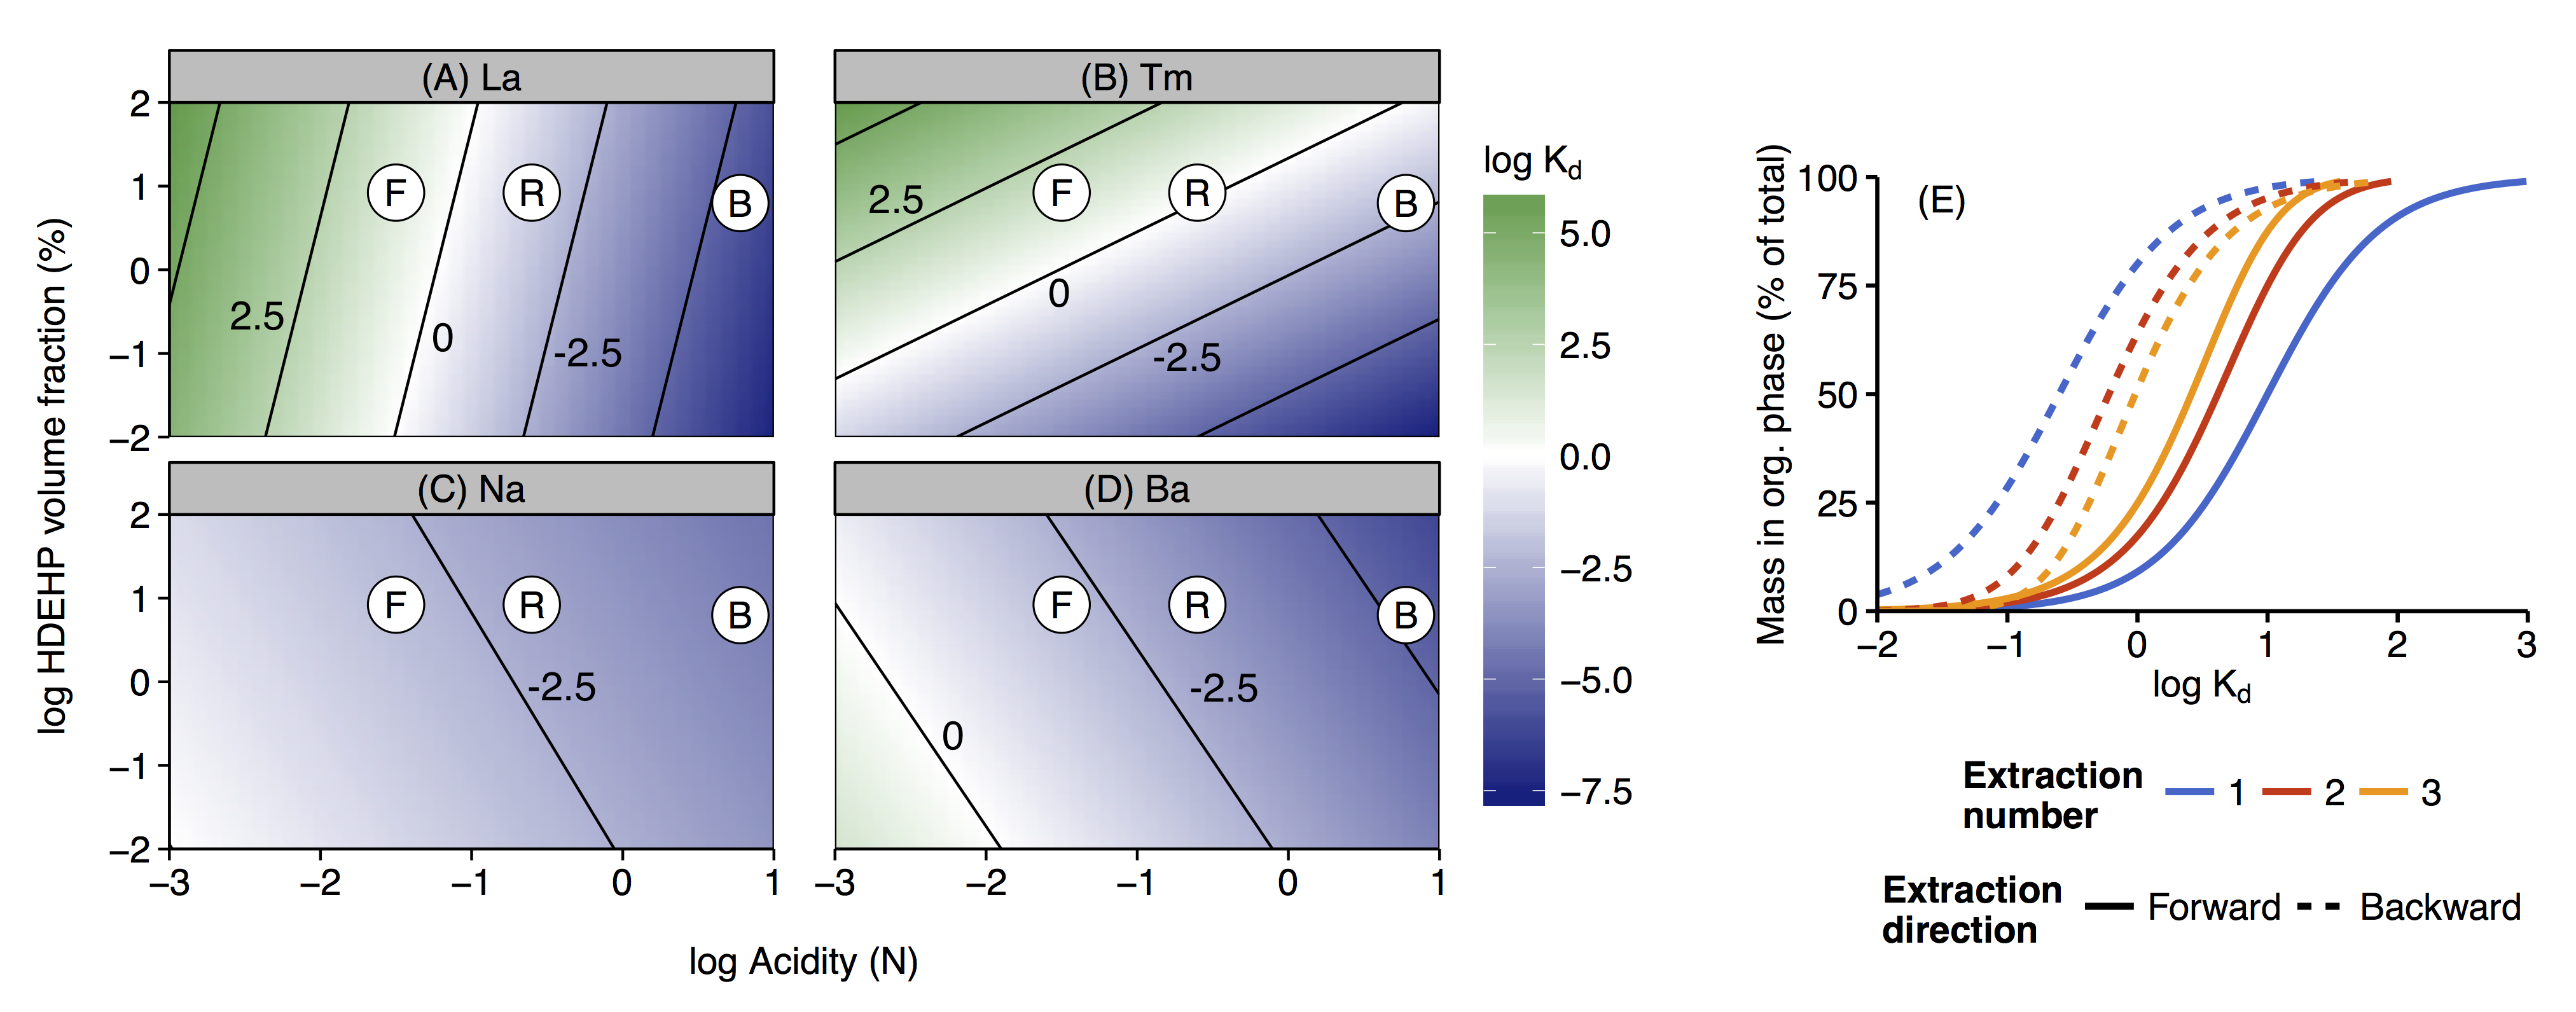
\includegraphics[width=\textwidth]{Ch4_figures/Kd-mod-plot.png}
\caption{Summary of model-based optimization of LLE operating conditions.
(A-D) Organic-aqueous distribution coefficient ($\log K_d$; Equation~\ref{eq:kimura_MLR}) contours as a function of acidity and HDEHP volume fraction for La, Tm, Na, and Ba calculated with data from Kimura \citep{Kimura_BCSJ_1960, Kimura_BCSJ_1961}.
LLE operating conditions for forward extractions (F), matrix rinse (R), and back extractions (B) suggested by Shabani et al. \citep{Shabani_AC_1990} are noted.
(E) Equilibrium partitioning for triplicate forward and backward extractions as a function of organic/aqueous distribution coefficient ($K_d$).
Partitioning calculated by Equation~\ref{eq:recovery} with $V_{aq}/V_{org} = 10$ for forward extraction and 0.25 for backward extraction.}
\label{fig:MLR-results}
\end{center}
\end{sidewaysfigure}


Using the equilibrium mass balance model (Equations~\ref{eq:recovery} and \ref{eq:step-recov}), the $K_d$ required to achieve the desired partitioning was matched to the results of this regression.
For each step of the LLE the desired partitioning is as follows:
\begin{enumerate}
	\item Forward extraction: Achieve high ($>99\%$) partitioning of the REE into the organic phase, while minimizing the partitioning of Ba and Na.
This can be achieved in a series of forward extractions.
	\item	Matrix rinse: Minimize partitioning of Ba and Na (i.e. low $K_d$) while maintaining a high ($>99\%$) partitioning of the REE. 
	\item Backward extraction: Minimize REE partitioning (i.e. leave $<1\%$ in the organic phase).
	This can be achieved in a series of backward extractions.
\end{enumerate}

Linear regression predicts a $\log_{10} K_d$ of 1.15 for La and 1.62 for Tm when using the conditions recommended by Shabani et al. \citep{Shabani_AC_1990}.
At these values, a mass balance model would predict 93\% partitioning in three forward extractions for La and exactly 99\% for Tm.
Similarly, in the recommended matrix rinse (0.25 N HCl) the model predicts $\log_{10} K_d$ of $-1.48$ for La and 0.21 for Tm, which correspond to 9\% retention of La in the organic phase and 83\% retention of Tm.
While this simplified analysis suggests that triplicate back extraction steps should achieve quantitative recovery of all REE ($\log_{10} K_d$ of $-2.18$ and $-5.57$ for La and Tm respectively), preliminary experiments (Figure~\ref{fig:reproduction}C and \ref{fig:reproduction}D) showed that the HREE were incompletely recovered. From these results an additional elution step was added to the procedure. 

From this analysis, it is clear that the $K_d$ values need to increase for forward extraction and the matrix rinse in order to achieve the desired partitioning at each step.
The LLE conditions, namely the solution acidity $[ACY]$, necessary to meet these goals can be found be examining the contours of Figure~\ref{fig:MLR-results}A,B and E .
Using Figure~\ref{fig:MLR-results}E it can be shown that forward extractions require $\log K_d>1.6$ to achieve $>99\%$ partitioning to the organic phase after triplicate extractions. Further, the conditions of the rinse phase must maintain $\log K_d>1.4$  to retain $>99\%$ REE in the organic phase from one rinse step. Finally, to achieve $>99\%$ recovery of REE during triplicate back extractions, conditions must create $\log K_d<-1.2$.
By decreasing the initial acidity to $<10^{-2}$ N (i.e. pH $>2$) the initial extraction of REE can be enhanced without significantly increasing partitioning of Na or Ba. From this analysis, an initial sample pH of 2.5 was chosen.
At a pH of 2.5 ($[ACY] = 10^{-2.5}$ N), forward extraction yields $\log K_d$ of 4.1 and 3.2 for La and Tm respectively.
Dissolution of the organic phase, which has been shown to diminish partitioning, should be limited below pH 3.54
Similarly, by reducing the acidity of the rinse step to $\leq10^{-1.5}$ N (i.e. pH $\geq1.5$) salts such as Na and Ba (Figures~\ref{fig:MLR-results}C and \ref{fig:MLR-results}D) can be eluted while retaining the REE (Figure~\ref{fig:MLR-results}A and \ref{fig:MLR-results}B).

\subsection{Interferences of synthetic brine constituents}

Results for REE recovery from simple solutions of 1 and 5 m NaCl, the REE are presented in Figure~\ref{fig:NaCl-only}.
In the 1 m NaCl solution, REE recovery was consistently between 90 and 110\%, however, indium recovery was markedly lower: 76 and 81\% in duplicate experiments.
Similar results were observed in the high salinity test (5 m NaCl), except that the heaviest two lanthanides, Yb and Lu, were recovered at a much lower rate, averaging 82\% for Yb and 72\% for Lu.
As the matrix rinse and back extraction conditions were identical between the 1 m and 5 m NaCl experiments, the diminished recovery is likely an artifact of diminished forward extraction and thus an effect of the increased salinity.
Recovery of indium from the 5 m NaCl solution (mean, 76\%) matched the recovery observed in the 1 m NaCl solution indicating that this diminished recovery is likely not a function of the salt concentration, and is instead endemic to indium in this extraction.

\begin{figure}[htbp]
\begin{center}
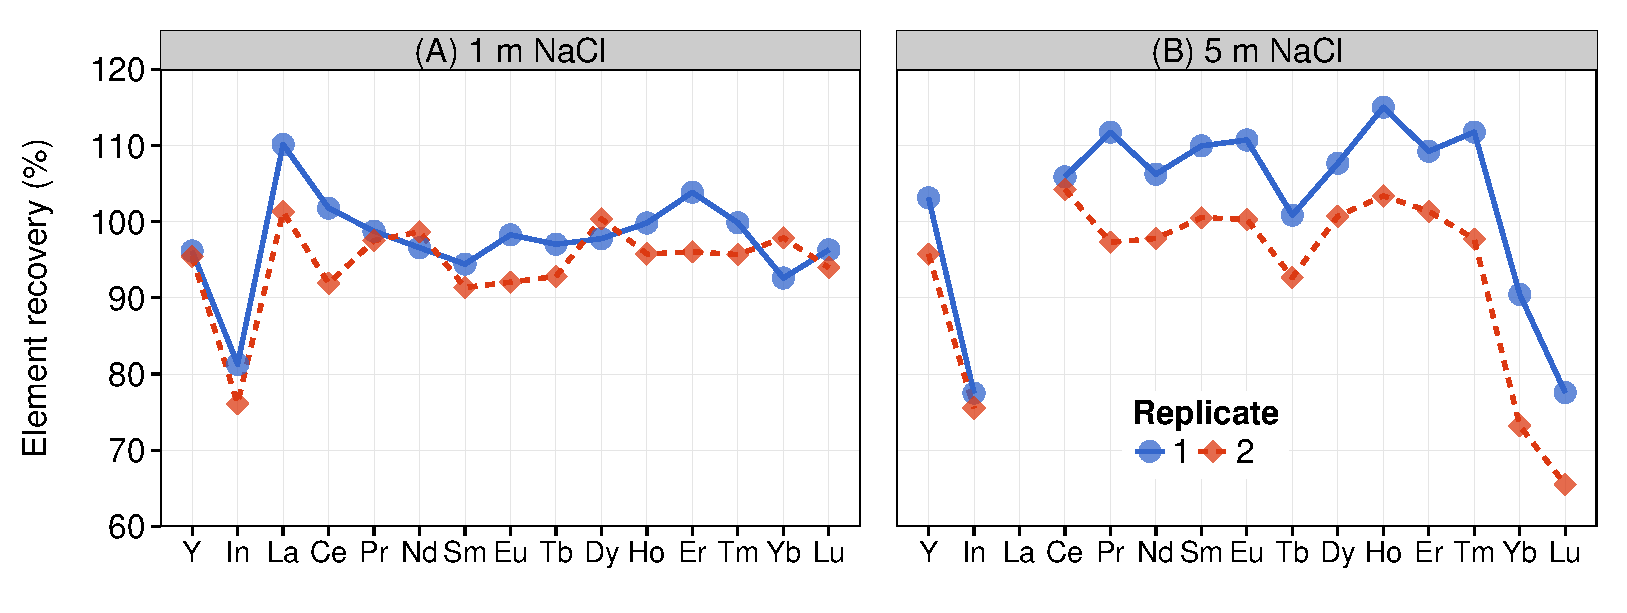
\includegraphics[width=\textwidth]{Ch4_figures/NaCl-only-LLE.pdf}
\caption{REE recovery by LLE method in simple, saline solutions.
Initial REE concentrations were 500 ppt (each element) in all experiments.
Duplicate experiments were conducted at each salinity and are represented by different line types, marker shapes, and colors.
Data for La in the 5 m NaCl experiment and for Gd in both experiments are excluded due to excessive background concentrations ($\geq250$ ppt).}
\label{fig:NaCl-only}
\end{center}
\end{figure}

Figure~\ref{fig:Doehlert-summary} summarizes the Doehlert design matrix experimental results, while experiment-ordered results, with replicates, are presented in Figure~\ref{fig:Doehlert-all}.
Data for Sc, La, and Gd are not included because these analytes were either not recovered (Sc, which is ``irreversibly bound'' in the organic phase \citep{Kimura_BCSJ_1960})
or contaminated by a high background (La and Gd; background $\geq 250$ ppt in all experiments).
Subsequent discussion excludes these elements.
Across all analytes, median recovery, $\widehat{Q}(0.50)=106\%$, was biased high (two-sided Wilcoxon Signed Rank test; H$_1$: $Q(0.5)\neq100\%$, $P < 10^{-6}$). However, these results are well within the recommended range of mean recovery for 1 ppb analytes (40 -- 120\% recommended) \citep{Taverniers_TrAC_2004}.
The absolute range of recoveries observed was 83-158\% while the reference range for recoveries (i.e the values between which 95\% of observations fell) was 92\% -- 122\%.
Experiments were generally reproducible (Figure~\ref{fig:Doehlert-all}), with element-specific, replicate standard deviations ranging from 0.05\% (Nd, experiment 4) to 21\% (In, experiment 1).
Finally, indium recovery was indistinguishable from any analyte (Wilcoxon, Rank-Sum test; $P>0.05$), in contrast to recovery from the simple NaCl solutions (Figure~\ref{fig:NaCl-only}).
Since these data are not sufficient to determine the mechanism by which this disparity was overcome, the application of indium as a tracer of REE recovery by the LLE method in unknown samples requires further study.

\begin{figure}[htbp]
\begin{center}
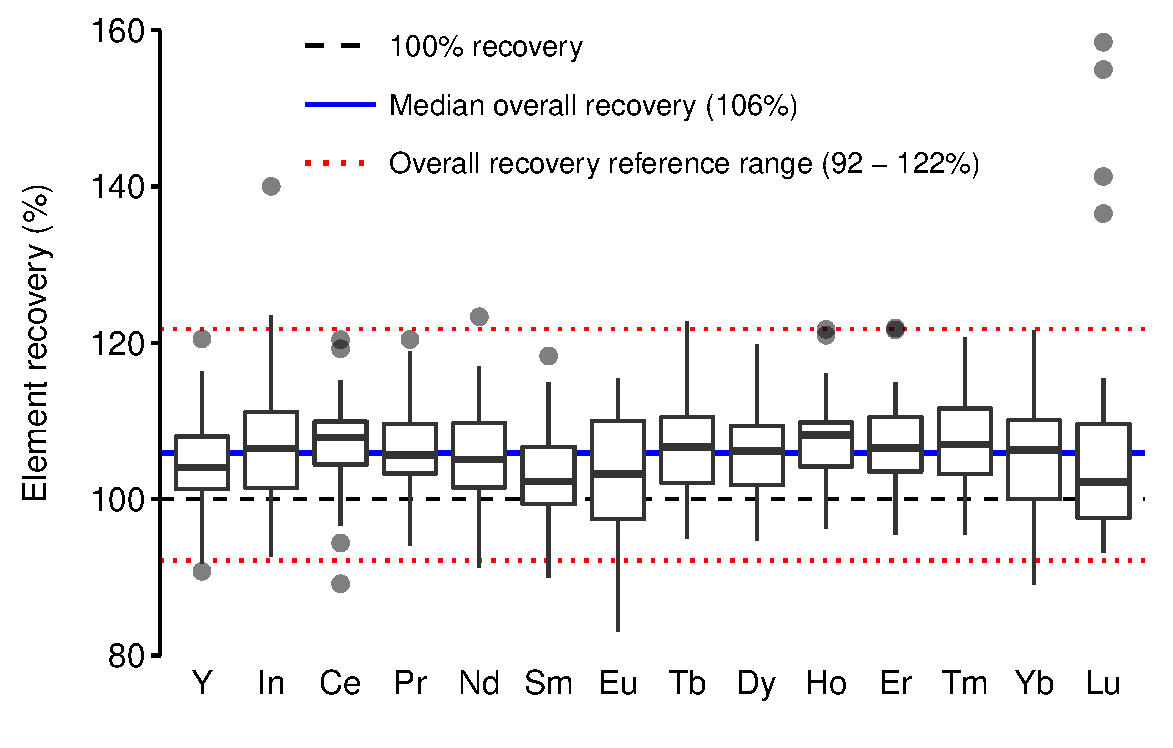
\includegraphics[width=0.8\textwidth]{Ch4_figures/Doehlert-results.pdf}
\caption{Distributions of elemental recovery in Doehlert matrix experiments by LLE methodology (see Figure~\ref{fig:Doehlert-all} for experiment-wise results). Distributions are depicted as standard box plots \citep{boxplots},
where the thick, black line depicts the median;
the boxed range represents the 25th to 75th percentile, or inter-quartile range (IQR);
the thin whiskers denote all measurements within 1.5 times the IQR above or below;
and the remaining observations are shown as semi-transparent grey dots.
Relevant summary statistics for the overall suite of analytes are given as horizontal lines.
Recovery values for Eu were determined after dosing the LLE eluent with \ce{H2SO4} to precipitate barite;
all other recoveries were determined without barite precipitation.
Data from La and Gd are not presented because the background concentration was determined to 250 ppt or greater (see Figure~\ref{fig:REE-bkgd}).}
\label{fig:Doehlert-summary}
\end{center}
\end{figure}


The data in Figure~\ref{fig:Doehlert-summary} and Figure~\ref{fig:Doehlert-all} indicate no clear fractionation (or mass bias) of the method across the suite of REE.
This result is confirmed by the Kruskal-Wallis test, which found no significant differences between any two element recoveries (H$_0$: No differences in element medians, $P > 0.1$).
Pairwise element testing (paired sample Wilcoxon Rank-Sum test, corrected for multiple comparisons) found statistically significant differences ($P < 0.05$) between 16 element pairs.
However, the differences were essentially indistinguishable from additive 3\% analytical errors (Figure~\ref{fig:element-diff-hist}).

\begin{figure}[htbp]
\begin{center}
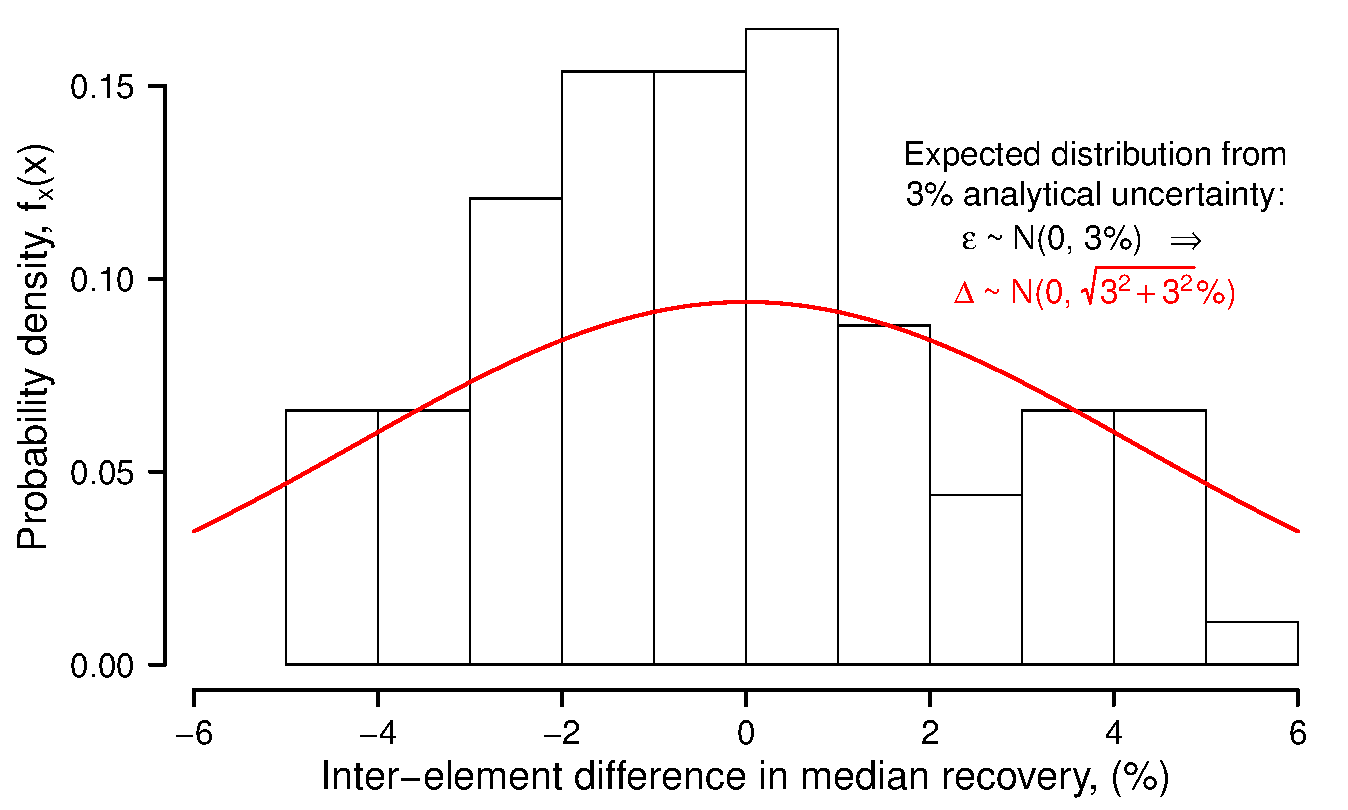
\includegraphics[width=0.75\textwidth]{Ch4_figures/element-diff-hist.pdf}
\caption{Comparison of pair-wise, inter-element differences in median recovery ($\Delta$, estimated from the paired-sample Wilcoxon Signed Rank test) to the expected (normal) distribution based on the difference between two random variates with equal means and 3\% analytical uncertainty, i.e.
$\Delta = N(\mu, 3\%) - N(\mu, 3\%) = N(0,\sqrt{3^2 + 3^2 }\%$).}
\label{fig:element-diff-hist}
\end{center}
\end{figure}


The lack of fractionation among REE in the more complex brines (i.e. with salinity, Fe, and DOC) differs from results obtained in experiments with simple NaCl solutions, where Yb and Lu recoveries were significantly lower at 5 m NaCl.
Step-wise regression analysis of element recovery (response) against solution composition (predictors) revealed no combination of linear- or interaction-terms among the study variables that substantially influenced recovery.
If the solution composition did have any impact on recovery within the range of parameters explored in the Doehlert design, it was indistinguishable from replicate variability.
These results give confidence to the application of the LLE methodology for natural samples with chemical characteristics within the bounds of the variables studied here, though accurate characterization of the REE concentration of unknown samples may require multiple replicates.

\subsection{Advice regarding natural samples}

Based on the results presented here, the modified LLE technique represents an attractive option for determination of REE in natural, hypersaline, and chemically complex brines.
However, it is critical to have accurate characterization of the samples of interest, as well as the oxide formation rates for the ICP-MS.
For samples with low Ba (i.e. a molar [Ba]:[Eu] $<10^5$ in raw samples), the addition of \ce{H2SO4} for barite precipitation is likely unnecessary if the available analytical instrumentation can maintain \ce{BaO+} interferences on the order of 0.1\% of analyte signal.
Samples with salinities and/or compositions outside of the range validated here may need to be tested with synthetic brines by the user.

While this study has explored the effects of DOC on LLE performance by way of a model compound, the character of DOC in the samples of interest should be considered more explicitly.
The effects of mixed organic components were not studied here.
Potent REE chelators can be found in other water sources, such as municipal wastewater discharges \citep{Bau_EPSL_1996,Kulaksiz_EPSL_2013}, and may have uncertain effects on the efficiency of REE recovery by this and other methods.

\bibliographystyle{unsrtnat}
\bibliography{Ch4_bib}

\begin{appendix}

\chapter{Supporting information for Chapter~\ref{chap:REE-review}}
\chaptermark{SI for REE in natural waters}
\section{Weighted Kaplan-Meier estimation of survival function for analyzing left-censored data}
\sectionmark{Analysis of left-censored data}

The weighted Kaplan-Meier (KM) estimator (\(\widehat{S}(x_i)\)) is expressed as:

\begin{align*}
\widehat{S}(x_i) = \prod_{x \geq x_i}\left(1 - \frac{d_i^w}{Y_i^w}\right)
\end{align*}

where, for application to aqueous chemistry data, \(\widehat{S}(x_i)\) is estimate of the probability of any measured concentration, \(x\), from the population being \emph{less} than \(x_i\).
It is calculated using the weighted count of uncensored observations at \(x_i\) (\(d_i\)) and the weighted count of all (censored or uncensored) observed concentrations less than \(x_i\) (\(Y_i^w\)).
The weighting of each data point is calculated here as the inverse of the number of samples from the data source, or \(w_i = n_i^{-1}\).
This curve can be used to estimate the quantiles of the data distribution as well as make estimates of the mean and variance of the population.
The computational methods here are adapted from Xie and Liu \citep{Xie_SiM_2005} and Singh et al. \citep{Singh_JAWMA_2013}.

To demonstrate these calculations, random data, drawn from log-normal distributions, will be used, followed by analysis of the groundwater REE dataset.
This analysis makes use of functions from the \texttt{plyr} (V 1.8.1), \texttt{dplyr} (V 0.3.0.2), and \texttt{tidyr} (V 0.1) packages which must be installed to run this analysis.
Aside from the pipe operator (\texttt{\%\textgreater{}\%}, loaded via the \texttt{dplyr} namespace, but part of the \texttt{magrittr} package), functions from these namespace are denoted as \texttt{package\_name::function\_name}, e.g. \texttt{dplyr::mutate}. 

Code, written in R, is shown with a grey-shaded background:

\begin{snugshade}
\begin{verbatim}
# This is an R comment
X <- 10
Y <- rnorm(1000)
\end{verbatim}
\end{snugshade}

Conversely, output from R calculations will be shown as:

\begin{verbatim}
##
## These are results
##
\end{verbatim}

\subsection{Generation of random data}
% Width of page (do not let code extend beyond)
% --------------------------------------------------------------------------------
\begin{snugshade}
\begin{verbatim}
## If these packages are not installed,
## un-comment and run these lines
# install.packages('plyr')
# install.packages('dplyr')
# install.packages('tidyr')
library(plyr)
library(dplyr)

# Data are drawn from three separate log-normal distributions
# Group means
means <- c(1,1.5,2.5)

# Samples in each group
N <- 100

# Generate random data
set.seed(8675309)
R <- data.frame(sapply(means, function(mu) rlnorm(N, mu, 1)))
colnames(R) <- c('Grp1','Grp2','Grp3')
head(R) # Look at first few values of random data, R

# `mutate` adds censoring and site ID
R.g <- tidyr::gather(data = R, key = Dataset,
                     value = Concentration,
                     contains('Grp')) %>%
         # Assume that 60% of samples were analyzed by
         # method with DL = 1 ppb, 40% with DL = 10 ppb
  dplyr::mutate(DL = sample(c(1, 10),
                            size = nlevels(Dataset)*N,
                            replace = T,
                            prob = c(0.6,0.4)),
         # Flag censored values and store at detection limit
         Censored = ifelse(test = Concentration < DL,
                           yes = 1, no = 0),
         Concentration = ifelse(Censored == 1,
                                DL, Concentration),
         # Randomly assign to sites w/ non-uniform probability
         Site = sample(LETTERS[1:10],
                       nlevels(Dataset)*N,
                       replace = T,
                       prob = 1:10/sum(1:10))) %>%
  dplyr::select(Dataset, Concentration, Censored, Site)

# Look at first few rows of fictional, partially censored data.
dplyr::tbl_df(R.g)
\end{verbatim}
\end{snugshade}

\begin{verbatim}
## Source: local data frame [300 x 4]
## 
##    Dataset Concentration Censored Site
## 1     Grp1        10.000        1    D
## 2     Grp1        10.000        1    J
## 3     Grp1        10.000        1    I
## 4     Grp1        20.685        0    H
## 5     Grp1         7.889        0    J
## 6     Grp1        10.000        1    I
## 7     Grp1         2.794        0    H
## 8     Grp1        10.000        1    I
## 9     Grp1         4.817        0    G
## 10    Grp1        10.000        1    F
## ..     ...           ...      ...  ...
\end{verbatim}

\subsection{Functions of the weighted Kaplan-Meier routine}

To utilize the weighted KM, the weights of each observation must be calculated.

\begin{snugshade}
\begin{verbatim}
calc_weights <- function(site_vector){
  counts <- data.frame(Site = site_vector) %>%
    dplyr::group_by(Site) %>% 
    dplyr::summarise(weight = 1/n())
  return(counts)
}

# Weights of sites are very similar across groups
# Note that no samples were assigned to "Site" A in Grp3,
# thus the weight is NA
plyr::ddply(R.g, .(Dataset), function(df){
    calc_weights(df$Site)
  }) %>%
  tidyr::spread(Dataset, weight)
\end{verbatim}
\end{snugshade}

\begin{verbatim}
##    Site    Grp1    Grp2    Grp3
## 1     A 0.25000 0.20000      NA
## 2     B 1.00000 0.20000 1.00000
## 3     C 0.16667 0.16667 0.20000
## 4     D 0.14286 0.16667 0.14286
## 5     E 0.25000 0.14286 0.08333
## 6     F 0.08333 0.08333 0.08333
## 7     G 0.12500 0.06667 0.12500
## 8     H 0.05000 0.10000 0.05263
## 9     I 0.06667 0.06667 0.05556
## 10    J 0.04348 0.05263 0.05556
\end{verbatim}

Next, the function for calculating the survival estimator is built.

\begin{snugshade}
\begin{verbatim}
Surv_weighted <- function(censored_data){
  # Data should have the following form [R data type]:
  # Column 1 = `Concentration` [double]
  # Column 2 = `Censored` [bool/int]
  # Column 3 = `Site` [factor]
  
  if(!is.factor(censored_data$Site)){
    censored_data$Site <- factor(censored_data$Site)
  }
  
  # Get weights
  site_weights <- calc_weights(censored_data$Site)
  
  # Combine weights with original data
  data_mod <- dplyr::left_join(censored_data,
                               site_weights,
                               by = 'Site')
  
  # Calculate the `at risk` observations, or
  # weighted # of observations less than each concentration
  data_mod <- dplyr::arrange(data_mod,
                             # Data in descending order
                             desc(Concentration)) %>%
    dplyr::mutate(Yw = sum(weight) - cumsum(weight) + weight)
  
  # Retain only uncensored (Censored == 0) observations
  observed <- dplyr::filter(data_mod, Censored == 0) %>%
    dplyr::select(-Censored)
  
  # All observations with identical values are counted
  obs_weight_tab <- dplyr::group_by(observed, Concentration) %>%
    dplyr::summarize(dw = sum(weight))
  
  # Combine weighted counts with rest of data and calculate S
  observed <- dplyr::left_join(observed, obs_weight_tab,
                               by = "Concentration") %>%
    # "incremental survival", value inside product
    dplyr::mutate(P = 1 - dw/Yw) %>%
    # Remove duplicated observations
    dplyr::filter(!duplicated(Concentration)) %>%
    dplyr:: mutate(S = cumprod(P),
                   S = ifelse(S<0,0,S))
  
  return(observed)
}
\end{verbatim}
\end{snugshade}

Using the simulated data, these functions can be tested:

\begin{snugshade}
\begin{verbatim}
# Calculate weighted KM for each dataset/group
sim_wKM <- R.g %>% plyr::ddply(.(Dataset), function(df){
  df <- dplyr::select(df,-Dataset)
  wKM <- Surv_weighted(df)
  return(wKM)
})

# Look at results
sim_wKM %>% 
  dplyr::select(Dataset, Concentration, weight, S) %>%
  dplyr::tbl_df()
\end{verbatim}
\end{snugshade}

\begin{verbatim}
## Source: local data frame [207 x 4]
## 
##    Dataset Concentration  weight      S
## 1     Grp1        20.685 0.05000 0.9950
## 2     Grp1        20.505 0.16667 0.9783
## 3     Grp1        19.803 0.08333 0.9700
## 4     Grp1        19.540 0.04348 0.9657
## 5     Grp1        14.310 0.06667 0.9590
## 6     Grp1        13.423 0.06667 0.9523
## 7     Grp1        13.130 0.04348 0.9480
## 8     Grp1        11.808 0.08333 0.9396
## 9     Grp1         9.981 0.25000 0.9038
## 10    Grp1         9.503 0.06667 0.8942
## ..     ...           ...     ...    ...
\end{verbatim}

To estimate the quantiles of a dataset with censoring, \texttt{Surv\_quantile} is defined, which calls \texttt{Surv\_weighted}.
This function will choose the observation closest to the desired quantile, without exceeding that quantile.
As in the main text, if the calculated survival quantiles, $S(x)$, for adjacent observations were $S(x_1)=0.94$ and $S(x_2)=0.96$, then $x_1$ would be noted as the 95$^{th}$ percentile.
If the desired quantile is outside of the range of calculated  (e.g. for $Q(0.05)$ when $\min \widehat{S}(x) > 0.05$), the quantile is estimated parametrically through regression on order statistics (ROS).
Here the data are assumed to be adequately fit by a log-normal distribution.
The parameters of this distribution are estimated from quantile-quantile regression.

\begin{snugshade}
\begin{verbatim}
Surv_quantile <- function(censored_data,
                          # Default to median + IQR
                          percentiles = c(0.25,0.5,0.75),
                          sig.fig = 3){
  # Fraction of data below detection
  cenfrac <- mean(as.logical(censored_data$Censored))
  
  # Calculate wKM and select relevant columnes
  weighted_km <- Surv_weighted(censored_data) %>%
    dplyr::select(Concentration, S)
  
  # Warnings about data
  if(any(cenfrac > percentiles)){
    warning(paste('The fraction of censored data is larger ',
                  'than one or more desired percentiles.\n',
                  'This may produce unreliable estimates.',
                  sep = ''))
  }
  
  out_of_range <- c(F,F)
  
  if(any(percentiles < min(weighted_km$S))){
    warning(paste('At least one desired percentile below', 
                  'minimum calculated from data,', 
                  'will be estimated from ROS.'), sep = ' ')
    out_of_range[1] <- T
  }
  
  if(any(percentiles > max(weighted_km$S))){
    warning(paste('At least one desired percentile above', 
                  'maximum calculated from data,', 
                  'will be estimated from ROS.'), sep = ' ')
    out_of_range[2] <- T
  }
  
  if(any(out_of_range)){
    ROS_data <- dplyr::filter(weighted_km, !is.na(S)) %>%
      transmute(y = log(Concentration), x = qnorm(S))
    ROS <- with(ROS_data,
                lm(y ~ x)
                )
    
    # Function for returning predictions based on ROS
    pred_ROS <- function(ROS_obj, percentile){
      new_dat <- data.frame(x = qnorm(percentile))
      log_pred <- predict(ROS_obj, newdata = new_dat)
      return(exp(log_pred))
  }
  
  fl.h <- function(percentile, S){
    h.temp <- which.min(abs(S - percentile))
    return(h.temp)
  }
  
  h.low <- sapply(percentiles, function(p){
      fl.h(p, weighted_km$S)
    })
  perc_df <- data.frame(Percentile = percentiles) %>%  
    dplyr::group_by(Percentile) %>%
    dplyr::mutate(h.low = fl.h(Percentile, weighted_km$S),
                  use_ROS = ifelse(
                    (Percentile < min(weighted_km$S) ||
                             Percentile > max(weighted_km$S)),
                     T,F)
                  ) %>%
    dplyr::ungroup() %>%
    dplyr::mutate(Xh = ifelse(use_ROS,
                              pred_ROS(ROS, Percentile),
                              weighted_km[h.low,
                                          'Concentration']),
                          Xh = signif(Xh, sig.fig)

  return(perc_df)
}
\end{verbatim}
\end{snugshade}

This estimation is demonstrated with the simulated data.
Note that in this example the rates of censoring are high in the first two groups, which elicits a warning from the \texttt{Surv\_quantile} code.
However, for clarity here, those warning messages have been suppressed.

\begin{snugshade}
\begin{verbatim}
plyr::ddply(R.g, .(Dataset),
      function(df){ 
        Surv_quantile(dplyr::select(df,-Dataset),
                      percentiles = c(0.05,0.25,0.5,0.75))
                         }) %>%
  dplyr::select(-h.low)
\end{verbatim}
\end{snugshade}

\begin{verbatim}
##    Dataset Percentile use_ROS     Xh
## 1     Grp1       0.05    TRUE  0.714
## 2     Grp1       0.25   FALSE  2.110
## 3     Grp1       0.50   FALSE  2.900
## 4     Grp1       0.75   FALSE  4.910
## 5     Grp2       0.05    TRUE  1.390
## 6     Grp2       0.25   FALSE  2.790
## 7     Grp2       0.50   FALSE  6.060
## 8     Grp2       0.75   FALSE  8.650
## 9     Grp3       0.05   FALSE  1.900
## 10    Grp3       0.25   FALSE  7.500
## 11    Grp3       0.50   FALSE 10.300
## 12    Grp3       0.75   FALSE 19.400
\end{verbatim}


\bibliographystyle{unsrtnat}
\bibliography{Ch4_appendix_bib}

\chapter{Supporting information for Chapter~\ref{chap:LLE}}
\chaptermark{SI for LLE method}
\section{Barium removal and background REE concentrations}
\sectionmark{Ba removal and REE background}

A primary objective in analyzing REE in natural water samples is the separation of Ba, which may lead to isobaric interferences with Eu.
Figure~\ref{fig:Ba-removal}A illustrates the effective rejection of Ba by the LLE method presented here, however Figure~\ref{fig:Ba-removal}C shows that even with $\sim0.2\%$ \ce{^{135}Ba^{16}O+}:\ce{^{135}Ba+}, the \ce{^{151}Eu+} is indistinguishable from \ce{^{135}Ba^{16}O+} in the vast majority of samples prior to barite precipitation.
Following precipitation (Figures~\ref{fig:Ba-removal}B,D), these issues are resolved.

\begin{figure}[htbp]
\begin{center}
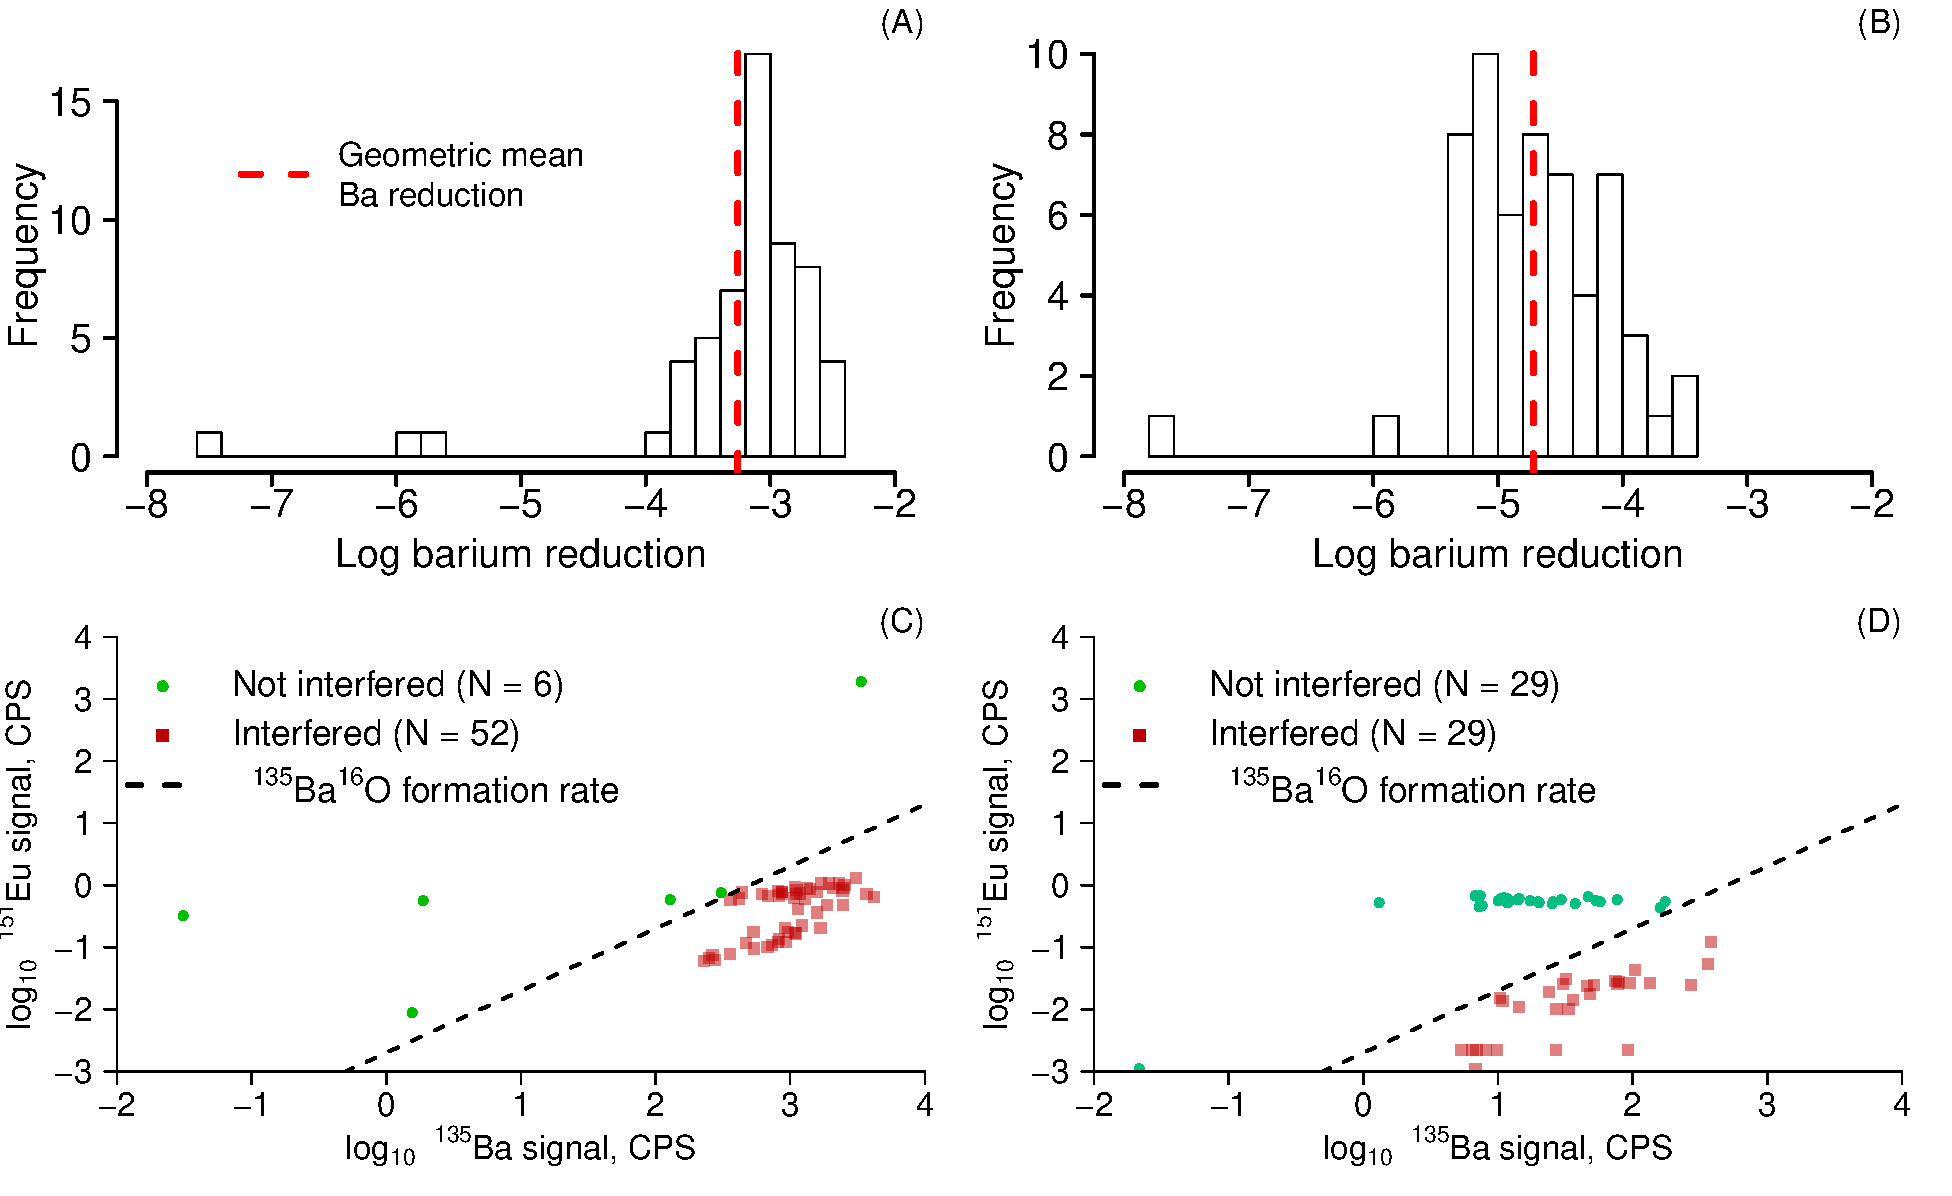
\includegraphics[width=0.8\textwidth]{Ch4_figures/Ba-removal.pdf}
\caption{Efficiency of Ba removal by LLE method (A, C) and ICP-MS octopole collision cell (B, D).
Results are for samples without (A, C) and with (B, D) \ce{H2SO4} addition to precipitate barite.
In (B) and (D), \ce{^{135}Ba^{16}O+} rate is inferred from 23 replicate analyses of a 200 ppb Ba standard after blank subtraction.
Interfered samples are those where accurate Eu determination could not be made due to excessive \ce{^{135}Ba^{16}O+} interference. In (D) the interfered samples were all unspiked experiments.}\label{fig:Ba-removal}
\label{default}
\end{center}
\end{figure}

Other experimental work in our shared lab space involves high concentrations ($\sim$mM) of Gd.
We ascribe the uniformly high Gd background in all experiments to cross contamination in this shared space.
In the ``Blank'' experiment (i.e. pH adjusted ASTM Type I water), all analytes were below detection (IDL $\sim$ 5 -- 20 ppt for 1\% false negative rate) except for Ba, La, and Gd. 
This indicates that the high La background could either be a result of laboratory cross-contamination (as with Gd) or an impurity in the organic phases used.
The latter supposition was investigated by direct contact of the mixed organic phases used (i.e. 3 mL 0.25 M HDEHP in heptane  + 1 mL octanol) with 4 mL of 6 N HCl, followed by analysis of the acid phase.
These results were below detection (not pictured), indicating no significant REE contamination of the organic phases.
While all chemicals were purchased at high purity, we can assume that the observed background concentrations in other experiments are due to trace contamination of these reagents.
Paradoxically, the level of these contaminations cannot be determined by ICP-MS without applying a separation/preconcentration technique such as the LLE method;
this makes source apportionment of the observed background concentration challenging.

\begin{sidewaysfigure}[htbp]
\begin{center}
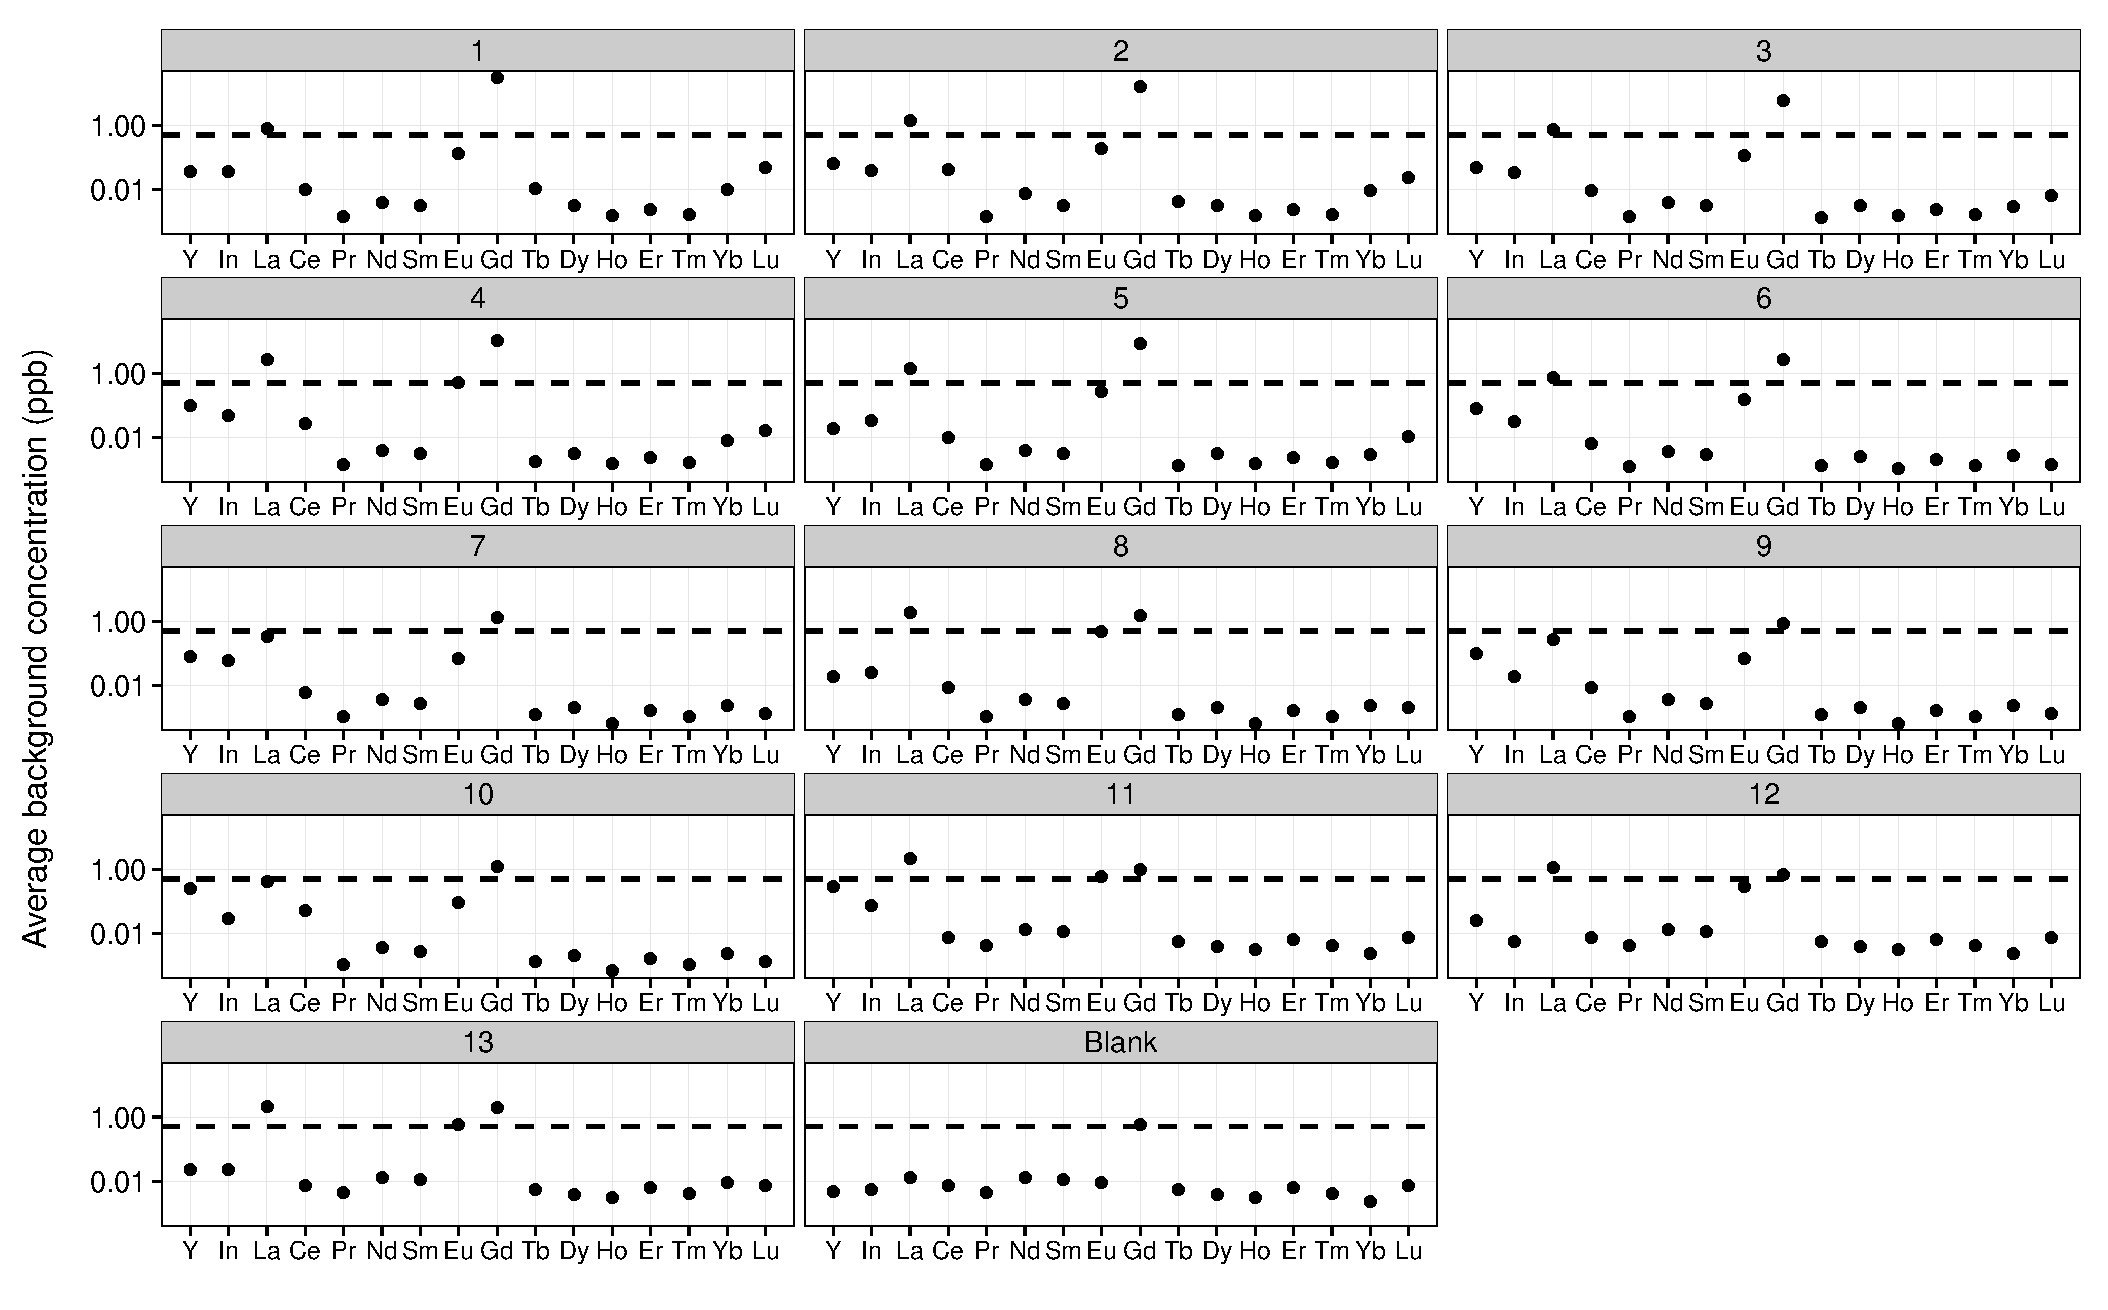
\includegraphics[width=0.95\textwidth]{Ch4_figures/REE-bkgd.pdf}
\caption{Average (from $n \geq 2$ replicates, except for Blank and experiments 6, 13) background concentrations of target analytes in samples without \ce{BaSO4} precipitation.
Dashed line at 500 ppt indicates the input concentration for all spiked samples.
Note that the y-axis is a logarithmic scale. Blank experiment represents pH adjusted ASTM Type I water.}\label{fig:REE-bkgd}
\end{center}
\end{sidewaysfigure}

\clearpage

\section{Doehlert experimental results}

These data represent the experiment and replicate ordered results of Doehlert matrix tests.
Each experiment number represents a unique set of solution conditions ([NaCl], [Fe], and [DOC]);
values for each of these parameters in each experiment is given in Table~\ref{tab:Doehlert}.

\begin{sidewaysfigure}[htbp]
\begin{center}
\includegraphics[width=\textwidth]{Ch4_figures/Exp-wise-LLE-recovery.pdf}
\caption{Elemental recovery in Doehlert matrix samples by LLE methodology (see Table~\ref{tab:Doehlert} for experimental conditions).
Recovery values for Eu were determined after dosing the LLE eluent with \ce{H2SO4} to precipitate barite;
all other recoveries were determined without barite precipitation.
Elements where the background concentration was determined to 250 ppt or greater (see Figure~\ref{fig:REE-bkgd}) were excluded (i.e. La and Gd in all experiments and Y in experiment 11).}
\label{fig:Doehlert-all}
\end{center}
\end{sidewaysfigure}



\end{appendix}

\end{document}